% !TEX root = ../geom_autistic_intro.tex
\section{Category Theory II}
\subsection{Limits and colimits}\label{Limits and colimits}

Recall the notions of products and coproducts, see Section \ref{Sec.Products}. We now generalize their construction to define limits and colimits of $\calJ$-shaped diagrams.

\begin{defn}[Limits and colimits]\index{Limit of a functor}\index{Colimit of a functor}
    Let $\mathcal{J}$ be an index category and $F$ a functor into any category $\mathcal{C}$, $F:\mathcal{J}\to \mathcal{C}$, thus representing a $J$-shaped diagram in $\mathcal{C}$ (see Def. \ref{categories of diagrams}). Then the limit
    \[\limit (F)\]
    is defined as the \emph{terminal object in the category of commutative cones} over the diagram $F(\mathcal{J})$, see Fig.\ \ref{fig:limits}. That is, it is an object  $L\in\ob(\calC)$ together with a collection of morphisms $L\overset{\psi_i}{\to}F(i)$ for each $i\in\ob(\calJ)$ such that each triangle 
    \[\begin{tikzcd}[every matrix/.append style={name=m},   
        execute at end picture={\draw [<-] ([xshift=13mm,yshift=0mm]m-2-2.north) arc[start angle=-90,delta angle=-270,radius=0.25cm];}]
        & L\arrow[dl,swap,"\psi_i" ]\arrow[dr,"\psi_j"] & \\
        F(i) \arrow[rr,swap,"f_{ij}"]& & F(j)
    \end{tikzcd}\]
    commutes and for any other object $A\in\ob(\mathcal{C})$ with a similar collection of morphisms $A\overset{\phi_i}\to F(i)$ there exists a unique morphism $A\to \limit (F)$ such that the entire diagram including $F(\mathcal{J})$, $\{\psi_i\}$, and $\{\phi_i\}$, commutes.
    
    Similarly, the colimit
    \[\colimit (F)\]
    is an initial co-cone (i.e.\ with morphisms pointing towards $L$) over $F(\mathcal{J})$. Like all universal objects, limits and colimits are defined uniquely up to a unique isomorphism (if they exist at all).
\end{defn}

\begin{figure}[tp]
    \centering
    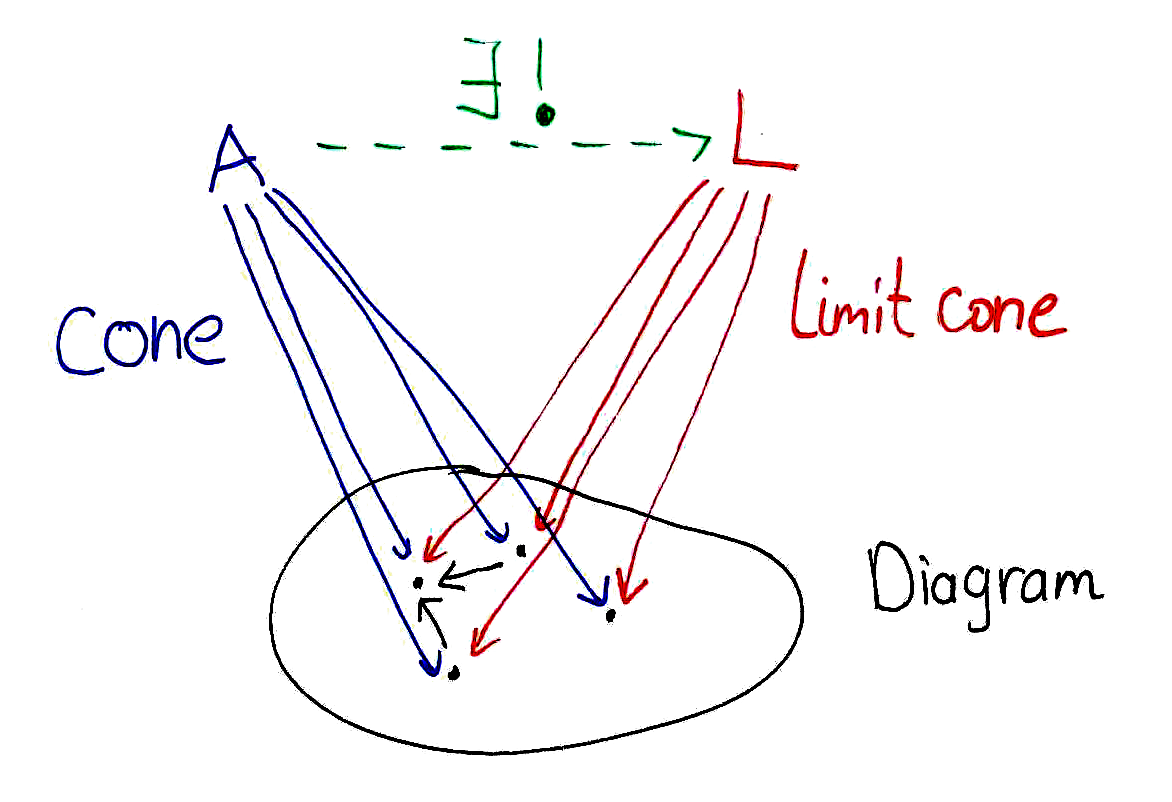
\includegraphics[scale=0.15]{figures/limits.png}
    \caption{Limit as the terminal cone over a diagram.}
    \label{fig:limits}
\end{figure}
    
\begin{example}
\begin{enumerate}
    \item $\calJ=\varnothing$ and $F$ is the empty functor into $\calC$. Then $\limit(F)$ is a terminal object in $\calC$ and $\colimit(F)$ is an initial object in $\calC$.
    \item $\calJ=(\bullet\quad\bullet)$ (discrete category with two objects). Then $\limit(F)=F(1)\times F(2)$ and $\colimit(F)=F(1)\sqcup F(2)$.
    \item $\calJ=(A\bullet\to \bullet_D\longleftarrow \bullet B$, then $\limit(F)=A\times_D B$.
    \item $F(\calJ)=(A\bullet\to \bullet B)$, then $\limit(F)=A$ and $\colimit{F}=B$.
    \item $F(\calJ)=(A\bullet\toto[\alpha]{\beta}\bullet B)$. Then $\limit(F)=\mathrm{eq}(\alpha,\beta)=\{a\mid \alpha(a)=\beta(a)\}$ is the equalizer and $\colimit(F)=\mathrm{coeq}(\alpha,\beta)=B/(\alpha(a)\sim \beta(a))$ is the coequalizer.

\end{enumerate}
\end{example} 

\begin{defn}[Preservation of limits]
    A covariant functor $G:\mathcal{C}\to\mathcal{D}$ preserves the limits of the functor $F:\mathcal{J}\to \mathcal{C}$ if $\limit(G\circ F)=G \limit(F)$. Recall that a limit consists of an object and a set of morphisms from that object that make up the limit cone, so $G$ also acts on these morphisms. Preservation of colimits is defined analogously.

    $G$ is said to preserve all $J$-shaped (co)limits if it preserves the (co)limits of all functors $F:\mathcal{J}\to \mathcal{C}$. 

    Note that for contravariant functors the analogous concepts would be functors that take limits to colimits, or colimits to limits.
\end{defn}    
\begin{defn}[Continuous functors]\index{Continuous functor}
    A functor is called (co)continuous if it preserves all \emph{small (co)limits} (that is, $J$-shaped (co)limits for all categories $J$ such that $\mathrm{Ob}(J)$ is a set and not a proper class).
\end{defn}
\begin{thm}[Continuity of hom-functors]
    Covariant hom-functors $h^A:B\mapsto \mathrm{Hom}_{\mathcal{C}}(A,B)$ preserve all limits. Similarly, contravariant hom-functors take colimits to limits.
\end{thm}
\begin{rem}
     Note that the same is not generally true for colimits -- e.g.\ $h^A(B\sqcup C)\neq h^A(B)\sqcup h^A(C)$ in $\mathsf{Set}$.
\end{rem}
\begin{cor}
    Combining the above theorem with Yoneda's Lemma \ref{Yoneda}, we conclude that all representable covariant functors preserve all limits. Similarly, representable contravariant functors map all colimits to limits.
\end{cor}
\begin{thm}\label{thm diagonal functor adjoint to limit}
    Recall that $\mathcal{C}^\mathcal{J}$ is the category of $J$-shaped diagrams in $\mathcal{C}$, i.e.\ covariant functors from $\mathcal{J}$ to $\mathcal{C}$ (see Example \ref{categories of diagrams}). Suppose that for each functor $F:\mathcal{J}\to\mathcal{C}$ the limit $\limit F$ exists in $\mathcal{C}$. Then the \emph{diagonal functor} which assigns to each object $A$ the \emph{constant diagram} $\underline A\in \mathcal{C}^\mathcal{J}$ (i.e.\ all objects of $\mathcal{J}$ are mapped to $A$ and all morphisms to $\mathrm{id}_A$),
    \[\Delta: \mathcal{C}\to \mathcal{C}^{\mathcal{J}};\; A\mapsto \underline{A},\]
    is left adjoint to the limit functor
    \[\limit: \mathcal{C}^\mathcal{J}\to \mathcal{C};\; F\mapsto \limit F\]
    (this functor forgets the morphisms associated with the limiting object).
\end{thm}
\begin{proof}
    For the bijection 
    \[
        \Hom_{\mathcal{C}^\mathcal{J}}(\underline{A},F)\cong \Hom_{\mathcal{C}}(A,\limit F),\label{limit functor bijection}
    \]
    note that a natural transformation $\tau: \underline{A}\Longrightarrow F$ (which is what morphisms in $\mathcal{C}^\mathcal{J}$ are) with component morphisms $\tau_j:A\to F(j)$ ($j$ ranges over all objects in $\mathcal{J}$) corresponds to a unique morphism $\limit \tau: A\to \limit F$ in $\mathcal{C}$. Conversely, a morphism $l:A\to \limit F$ determines a unique natural transformation $\tau:\underline{A}\Longrightarrow F$ such that $l=\limit \tau$, namely its components are $\tau_j=l\pi_j$ given the morphisms $\pi_j$ included in the definition of $\limit F$. It is easy to check that this bijection is natural in $A$.
\end{proof}
\begin{cor}\label{corollary on limits}
    The natural bijection (\ref{limit functor bijection}) (with some object $L$ from $\mathcal{C}$ instead of $\limit F$ to avoid confusion) holds for each object $A$ in $\mathcal{C}$ iff the functor $F$ has a limit.
\end{cor}
\begin{proof}
    The existence of the limit is equivalent to the existence of a unique morphism $\limit \tau: A\to L$ for each natural transformation $\tau:\underline{A}\to F$.
\end{proof}
\begin{rem}
    Since a morphism (natural transformation) $\underline{A}\Longrightarrow F$ in the category $\mathcal{C}^\mathcal{J}$ is the same as a cone from $A$ to $F$, the limit $\limit F$ can be defined as the universal natural transformation $\Delta \Longrightarrow F$. Similarly, colimits are the universal natural transformations $F\Longrightarrow \Delta$.
\end{rem}
\begin{thm}[Continuity of adjoint functors]\label{continuity of adjoints thm}
    Every functor that has a left adjoint (and therefore is a right adjoint) is continuous. The dual statement is that every functor that has a right adjoint (and therefore is a left adjoint) is cocontinuous.
\end{thm}
\begin{proof}
    Let $R:\mathcal{C}\to \mathcal{D}$ be the right adjoint to $L:\mathcal{D}\to\mathcal{C}$. Suppose that $\limit F$ exists in $\mathcal{C}$. For each object $A$ in $\mathcal{C}$, a natural bijection
    \[\Hom_{\mathcal{C}^\mathcal{J}}(\underline{L(A)},F)\cong \Hom_{\mathcal{D}^\mathcal{J}}(\underline{A},R\circ F) \label{adjunction bijeciton}\]
    is provided by the natural adjunction bijection
    \[\Hom_{\mathcal{C}}(L(A),F(j))\cong \Hom_{\mathcal{D}}(A,R(F(j))\]
    for each object $j$ in $\mathcal{J}$, sending the component $h_j$ of an element of the l.h.s.~of (\ref{adjunction bijeciton}) to the corresponding component of the natural transformation on the right. Now consider the string of natural bijections
    \begin{multline}
        \Hom_{\mathcal{D}^\mathcal{J}}(\underline{A},R\circ F)\cong \Hom_{\mathcal{C}^\mathcal{J}}(\underline{L(A)},F)\cong \\ 
        \cong \Hom_{\mathcal{C}}(L(A),\limit F)\cong \Hom_{\mathcal{D}}(A,R(\limit F))
    \end{multline}
    coming respectively from (\ref{adjunction bijeciton}), (\ref{limit functor bijection}), and the adjunction. By Corollary~\ref{corollary on limits} combined with the uniqueness of adjoints (Proposition~\ref{uniqueness of adjoints prop}), we have $\limit(R\circ F)= R(\limit F)$ as required.
    % Let $G:\mathcal{D}\to\mathcal{C}$ be a left adjoint, i.e.\ $G^\ast$ exists. Then for a colimit $\colimit(F)$ of $F:\mathcal{J}\to \mathcal{D}$, by continuity of hom-functors, we have
    % \begin{multline}
    %     \Hom_{\mathcal{C}}(G\colimit F,B)\cong \Hom_{\mathcal{D}}(\colimit F,G^\ast(B))\cong \limit \Hom_{\mathcal{D}}(F,G^\ast(B)) \cong \\\cong \limit \Hom_{\mathcal{C}}(G\circ F,B)\cong \mathrm{Cocones}(G\circ F,B),
    % \end{multline}
    % and these bijections are natural in $B$. However, the existence of a natural bijection with the set of cones from $G\circ F$ is exactly the characteristic property of a colimit (see definition).
\end{proof}
\begin{cor}
    Limits commute with limits (assuming all limits of the necessary shapes exist). Colimits commute with colimits.
\end{cor}
\begin{proof}
    Viewing the limit is a functor  $\limit:\calC^J\to \calC$, we have just shown that it is right adjoint to the diagonal functor (a.k.a.~the constant diagram functor). Therefore it is continuous, i.e.~commutes with limits. 
\end{proof}

Note that limits and colimits typically do not commute.

\begin{example}[Siefert-van Kampen theorem redux]\index{Theorem!Siefert-van~Kampen}
    We've learned by now that contravariant representable (or hom-) functors map colimits to limits, so they're not the functors that preserve colimits. It is the left adjoints that do. Siefert-van~Kampen theorem essentially states that the fundamental functors $\pi_1$ or $\Pi$ preserve \emph{some} colimits (namely pushouts). 
    
    While not a proof, one categorical source of intuition for this is that both of these functors are left adjoints. The reason $\pi_1$ preserves only pushouts, and not all colimits, is that the functor that maps the category $\mathsf{Top}$ into the homotopy category $\mathsf{hTop}$ doesn't preserve colimits, so $\pi_1$ doesn't either. However, the descended version of this functor, $\pi_1:\mathsf{hTop}\to \mathsf{Gr}$ happens to be the left adjoint of a certain functor that constructs a topological space given a group. Looking far ahead, this is the functor $B:G\mapsto BG$ that constructs the classifying space of $G$. It is so called because $BG$ is the base space of a universal principal $G$-bundle such that any other $G$-bundle is a pullback along some continuous map into $BG$. For example, universal covering spaces are exactly the classifying spaces for the fundamental groups of their base -- e.g.\ $B\bbZ=\bbS^1$ and $B(\bbZ\ast \bbZ)=\bbS^1\vee \bbS^1$ etc. $BG$ is in fact the unique (up to ``weak'' homotopy equivalence) space whose fundamental group is $G$ and all other homotopy groups are trivial (which also identifies it with the first  Eilenberg-MacLane space $K(G,1)$).

    So, by a happy coincidence, pushouts in the homotopy category lined up with pushouts in the original topological category.
\end{example}

The most common examples of infinite limits and colimits are ones where $\mathcal{J}$ can be indexed by integers.

\begin{defn}[Direct and inverse limits]\index{Limit!direct}\index{Limit!inverse}
    If $\calJ$ is a directed system and $F:\calJ\to \calC$ a functor, then $\colimit(F)$ is called a direct, or an inductive, limit. It is also often written as $\colimit A_j$, where $A_j=F(j)$.
    
    If $\calJ$ is an inverse system (i.e.~$\calJ^{\mathrm{op}}$ is a directed system), then $\limit(F)$ is called an inverse, or a projective, limit.
    
    More generally, if $\calJ$ is a poset category (see Example \ref{poset example}), then it is said to be directed to the right (left) if $\forall i,j\in \ob(\calJ)$ $\exists k\in \ob(\calJ)$ such that $i,j\leq k$ (respectively, $k\leq i,j$). Then one can define direct limits of diagrams directed to the right and inverse limits of diagrams directed to the left.
\end{defn}


\begin{example}
\begin{enumerate}
    \item In $\colimit$, most commonly all arrows are monomorphisms. For example, consider the category $\mathsf{Gr}$ of groups and the sequence $S_n$ of symmetric groups with the embeddings $S_n\hookrightarrow S_m$ for every $n<m$ defined as permutations of the first $n$ symbols. Then $\colimit(S_n)=S_\infty$, which is the group of all permutations of $\mathbb{N}$ of finite support.
    
    Alternatively, we can define another partial order on the set of symmetric groups $S_n$. Namely, define $n\preccurlyeq m\Leftrightarrow n\mid m$ and the inclusion $S_n\hookrightarrow S_m$ by $m/n$ copies of the permutation. Then $\colimit (S_n)$ is a different group.
    \item For any unital ring $R$, the direct limit of the general linear matrix groups over $R$ (where matrices of size $n$ are embedded into groups of larger matrices by filling in the diagonal with ones) is $\colimit(\GL(n,R))=\GL(R)$, the \emph{quite general linear group} of $R$.
    \item In $\mathsf{Set}$, direct limits are simply infinite unions factored by identifying elements with coincident ``descendants'', i.e. $\colimit A_i=\bigsqcup_i A_i/\sim$, where $x\in A_i$ is equivalent to $y\in A_j$ iff $\exists f_{jk},f_{jk}$ such that $f_{ik}(x)=f_{jk}(y)$. The inverse limit is the set of infinite sequences of descendants $\limit (A_i)=\{(a_i)\mid a_i\in A_i,\forall i\leq j, f_{ij}(a_i)=a_j\}$.
    \item Consider the polynomial ring $K[t]$ over a field $K$ and its factor rings $K[t]/t^n$ of truncated polynomials. Then we have the sequence of epimorphisms 
    \[\cdots \to K[t]/t^3\to K[t]/t^2\to K,\]
    and the inverse limit is $\limit(K[t]/t^n)=K[[t]]$, which is the ring of \emph{all} formal power series $\sum_{i\geq 0}a_i t^i$. This illustrates the more general fact that projective limits are generally enormous, so much so that the cardinality of the limit is often higher than of any object in the sequence.
    \item Let $p$ be a prime integer and consider the sequence of groups
    \[\cdots\to \bbZ/p^3 \bbZ\overset{\mod p^2}\to \bbZ/p^2\bbZ\overset{\mod p}\to \bbZ/p\bbZ.\]
    Then $\limit(\bbZ/p^n\bbZ)=\bbZ_p$ is the group of $p$-adic integers (it has the cardinality of continuum!).
    \item Consider the poset diagram directed to the left consisting of group epimorphisms $\bbZ/m\bbZ\overset{\mod n}\to \bbZ/n\bbZ$ for $n\mid m$. Then 
    $\limit (\bbZ/n\bbZ)=\hat{\bbZ}$ is the \emph{profinite completion of $\bbZ$}.
    \item The monomorphism sequence $\bbZ/p^n\bbZ\overset{\cdot p}\to \bbZ/p^{n+1}\bbZ$ gives the direct limit $\colimit(\mathbb{Z
    }/p^n\bbZ)=\bbZ(p^\infty)$, which is called a Pr\"ufer group (it can be realized as the group of all roots of unity of the form $\exp(2\pi\rmi \cdot m/p^n)$).
    \item In topological and geometric categories, direct limits are similar to unions (when they exist). For instance, the $n$-sphere can be embedded $\bbS^n\hookrightarrow \bbS^{n+1}$ as the equator, and the direct limit gives $\bbS^\infty=\colimit \bbS^n$.
\end{enumerate}
\end{example}





\subsection{Sub-objects and quotient objects}

\begin{defn}
    Let $X,U,V\in\ob(\calC)$ and consider a diagram
    \[\begin{tikzcd}[every matrix/.append style={name=m},   
        execute at end picture={\draw [<-] ([xshift=-2mm,yshift=-12mm]m-1-2.north) arc[start angle=-90,delta angle=-270,radius=0.25cm];}]
        U \arrow[dr,tail,"u\text{, mono}"]& \\
        & X\\
        V\arrow[uu,tail,dashed,"\exists h"]\arrow[ur,tail,swap,"v\text{, mono}"]& 
\end{tikzcd}\]
    We say that $v\leq u$ if there exists a morphism $h$ such that $v=u\circ h$ ($h$ has to be a monomorphism for this to hold).
\end{defn}

Here are the properties of this relation:
\begin{enumerate}
    \item $u\leq u$;
    \item $u\leq v,v\leq w\Rightarrow u\leq w$;
    \item $u\leq v,v\leq u\Rightarrow U\overset{f}{\cong} V$, where $u=v\circ f$ and $v=u\circ f^{-1}$.
    \begin{proof}
        We have $V\overset{h}{\to}U$ and $U\overset{g}{\to}V$.
        
        On the one hand, $v=u\circ h=v\circ g\circ h\Rightarrow g\circ h=1_V$ since $v$ is mono.
        
        On the other hand, $u=u\circ(h\circ g)\Rightarrow h\circ g=1_U$ since $u$ is mono.
    \end{proof}
\end{enumerate}

\begin{defn}[Sub-objects]\index{Sub-object}
    Introduce an equivalence relation on monomorphisms: $u\sim v$ iff $u\leq v$ and $v\leq u$. Then a sub-object of $X$ is an equivalence class of pairs $(U,u)$, where $u:U\to X$ is a mono.
\end{defn}

\begin{example}
    $\bbZ\overset{\cdot n}\to \bbZ$ is mono and defines the group $n\bbZ$ as a sub-object of $\bbZ$.
\end{example}

\begin{defn}[Quotient objects]\index{Quotient object}
    For epimorphisms, we define the relation $y\geq z$ if in the diagram 
    \[\begin{tikzcd}[every matrix/.append style={name=m},   
        execute at end picture={\draw [<-] ([xshift=-6mm,yshift=-5mm]m-2-2.north) arc[start angle=-90,delta angle=-270,radius=0.25cm];}]
        & Y \arrow[dd,two heads,dashed,"\exists h"] \\
        X\arrow[dr,two heads,swap,"z\text{, epi}"]\arrow[ur,two heads,"y\text{, epi}"] &\\
        & Z 
    \end{tikzcd}\]
    there exists such a morphism $h$ that $z=h\circ y$ (it has to be epi).
    Then a quotient object of $X$ is an equivalence class of pairs $(Y,y)$, where $y:X\to Y$ is epi.
\end{defn}

\begin{example}
    There are many different epimorphisms $\bbZ^2\to\bbZ$. They define many non-equivalent quotient objects of $\bbZ^2$, each isomorphic to $\bbZ$.
\end{example}



\subsection{Abelian categories}

Abelian categories are, roughly speaking, categories where objects and morphisms form abelian groups themselves, and where the First Isomorphism theorem holds. Examples include $\mathsf{Ab}$, $\mathsf{Vect}_K$, $R-\mathsf{Mod}$ or $\mathsf{Mod}-R$, $\mathsf{SheafAb}$. Notably, $\mathsf{TopAb}$ is not abelian because the First Isomorphism theorem generally doesn't hold for topological groups (we call such a category pre-abelian).

\begin{defn}[Abelian categories]\index{Abelian category}
    A category $\calC$ is called abelian if:
    \begin{enumerate}
        \item Every morphism set $\mor(A,B)$ has the structure of an abelian group, i.e. morphisms can be added and subtracted.
        \item There exists a zero object $0\in\ob(\calC)$.
        \item The product and coproduct of any two objects exist and are isomorphic. The result is denoted by the direct sum: $A\times B\cong A\sqcup B \equiv A\oplus B$.
        \item All equalizers and coequalizers exist. In particular, using the abelian property, we define
        \[\ker (\varphi)\coloneqq\mathrm{eq}(\varphi,0),\quad \coker(\varphi)\coloneqq\mathrm{coeq}(\varphi,0).\]
        \item The image and coimage of any morphism coincide, $\im (\varphi)=\coim(\varphi)$. These will be defined below.
    \end{enumerate}
\end{defn}

We can give alternative definition of kernels and cokernels.
\begin{defn}[Kernel]\index{Kernel}
    Let $X\overset\varphi\to Y$ be a morphism in an abelian category. Then $\ker\varphi$ is the sub-object $(K,k)$ of $X$ such that $\varphi\circ k=0$ and it is universal with this property:
    \[\begin{tikzcd}[every matrix/.append style={name=m},   
        execute at end picture={\draw [<-] ([xshift=-10mm,yshift=-8mm]m-1-2.north) arc[start angle=-90,delta angle=-270,radius=0.15cm];}]
        K \arrow[r,tail,"k"]& X\arrow[r,"\varphi"] & Y\\
        Z\arrow[u,dashed,"\exists! h"]\arrow[ur,swap,"\forall\psi:\,\varphi\circ\psi=0"]& & 
    \end{tikzcd}\]
    (such a $h$ is automatically unique for every $\psi$ because $k$ is mono).
\end{defn}

\begin{defn}[Cokernel]\index{Cokernel}
    Let $X\overset\varphi\to Y$ be a morphism in an abelian category. Then $\coker\varphi$ is the quotient object $(C,c)$ of $Y$ such that $c\circ\varphi=0$ and it is universal with this property:
    \[\begin{tikzcd}[every matrix/.append style={name=m},   
        execute at end picture={\draw [<-] ([xshift=-4mm,yshift=-8mm]m-1-3.north) arc[start angle=-90,delta angle=-270,radius=0.15cm];}]
        X\arrow[r,"\varphi"] & Y \arrow[r,two heads,"c"]\arrow[dr,swap,"\forall\psi:\,\psi\circ\varphi=0"]  & C\arrow[d,dashed,"\exists! h"] \\
        & & Z
    \end{tikzcd}\]
    (such a $h$ is automatically unique for every $\psi$ because $c$ is epi).
\end{defn}

\begin{example}
    It is easy to check that in the category $\mathsf{Ab}$ of abelian groups, $\coker\varphi=H/\varphi(G)$ for $\varphi:G\to H$. Thus the last axiom of abelian categories is equivalent to the First Isomorphism theorem in this case. Note that this factor doesn't exist neither in $\mathsf{Gr}$ nor in $\mathsf{TopAb}$.
    
    The same formula holds for all ring modules. In $\mathsf{Gr}$ (which is not an abelian category, but in which kernels and cokernels can be similarly defined), the cokernel is the quotient by the normal closure of the image.
\end{example}

This allows us to define images and coimages.

\begin{defn}[Image, coimage]\index{Image of a morphism}\index{Coimage of a morphism}
    In abelian categories, $\im\varphi$ for a morphism $\varphi:X\to Y$ is the sub-object of $Y$ defined as
    \[\im(\varphi)=\ker(\coker\varphi),\quad\quad K\overset k \rightarrowtail X\overset\varphi\to Y\overset c\twoheadrightarrow C.\]
    Similarly, $\coim\varphi$ is the quotient object of $X$ defined as 
    \[\coim(\varphi)=\coker(\ker\varphi).\]
\end{defn}

Note that
\[\ker(\coim\varphi)=\ker(\coker(\ker\varphi)))=\im(\ker\varphi).\]
Thus in general pre-abelian categories (i.e.\ without the last axiom) by the universal properties of images and coimages we have a factorization of any morphism $\varphi:X\to Y$ into the sequence
\[\ker\varphi\rightarrowtail X\underbrace{\overset{\text{epi}}\twoheadrightarrow\coim\varphi\overset{\text{bi}}\to\im\varphi\overset{\text{mono}}\rightarrowtail}_\varphi Y\twoheadrightarrow\coker\varphi \]
The last axiom of abelian categories states that $\coim\varphi = \im\varphi$, which is equivalent to the statement:
\[\boxed{\text{5. All bimorphisms are isomorphisms.}}\]
\begin{xca}
    Prove that the last axiom of abelian categories is indeed equivalent to the boxed statement.
\end{xca}
Therefore only in abelian categories we have the decomposition
\[\ker\varphi\to X \overset{j\text{, epi}}\longrightarrow\im\varphi\overset{i\text{, mono}}\longrightarrow Y\to \coker\varphi,\]
where
\[\text{factorization property}:\quad \varphi=i\circ j,\quad i\text{ -- mono}, j\text{ -- epi}.\]

\begin{defn}[Additive functor]
    A functor $F:\calC\to\calD$ between two abelian categories is called additive if for any $A,B\in\ob(\calC)$, the map $F_{A,B}:\Hom_\calC(A,B)\to \Hom_\calD(F(A),F(B))$ defined by $\varphi\mapsto F_{A,B}(\varphi)=F(\varphi)$ is a homomorphism of abelian groups.
\end{defn}

The following theorem is the main general result about abelian categories and effectively states that all abelian categories can be realized as (almost arbitrarily nice) full subcategories of categories of ring modules. It is essentially a much stronger version of the Yoneda Lemma~\ref{Yoneda} for abelian categories.

\begin{thm}[Freyd-Mitchell]
    For any abelian category $\calC$ there exists a ring $R$ and a functor $F:\calC\to R\text{-}\mathsf{Mod}$ that is: additive, full and faithful (surjective and injective on sets of morphisms for each pair of objects), preserves kernels, cokernels, products and coproducts, is exact (preserves exact sequences, see below)...
\end{thm}
This theorem justifies all diagrammatic methods that we will develop in the next two sections: since $R\text{-}\mathsf{Mod}$ is a concrete category, its objects are sets. Therefore by the Freyd-Mitchell theorem, it suffices to prove any general statement about abelian categories only for categories of ring modules, which allows us to refer to elements of objects as sets, and apply morphisms as functions to those elements! It is a way to completely side-step so called ``abstract nonsense'' proofs that deliberately avoid talking about elements of objects as if they are sets.






\newpage
\section{Homological Algebra I: Exactness}

\subsection{Exact sequences and functors}

From now on in this Part we work only with abelian categories. In fact, homological algebra can be viewed as the extension of linear algebra to all abelian categories.

\begin{defn}[Exact sequences]\index{Exact sequence}
    A sequence of morphisms in an abelian category 
    \[\cdots \to A_{i-1}\overset{\alpha}\to A_i\overset{\beta}\to A_{i+1}\to \cdots\]
    is called exact in $A_i$ if 
    \[\im\alpha=\ker\beta.\]
    A sequence is just called exact if it is exact in every object in it.
\end{defn}

\begin{prop}
    \begin{enumerate}
        \item A sequence $0\to A\overset f\to B$ is exact iff $f$ is mono;
        \item A sequence $A\overset f\to B\to 0$ is exact iff $f$ is epi;
        \item A sequence $0\to A\overset f\to B\to 0$ is exact iff $f$ is an isomorphism;
        \item A sequence $0\to A\to B\overset f\to C\to D\to 0$ is exact iff $A=\ker f$ and $D=\coker f$.
    \end{enumerate}
\end{prop}
\begin{proof}
    Exercise.
\end{proof}

\begin{defn}[Short exact sequences]\index{Exact sequence!short}
 A short exact sequence is an exact sequence of the form
 \[0\to A\overset f\rightarrowtail B\overset g \twoheadrightarrow C\to 0.\]
 Such a sequence (and the object $B$ in particular) is also called an \emph{extension} of $A$ by $C$. The exactness of this sequence is equivalent to $f$ being mono, $g$ being epi, and $\im f=\ker g$.
\end{defn}

\begin{prop}[First isomorphism theorem]
    If $0\to A\overset f\to B\overset g \to C\to 0$ is a short exact sequence, then 
    \[A\cong \im f,\quad C\cong B/\im f.\]
\end{prop}
\begin{proof}
    The first isomorphism is known in concrete categories, which is sufficient. It states that $B/\ker g\cong \im g$, and by exactness $\ker g=\im f$ and $\im g=C$, thus $B/\im f\cong C$.
\end{proof}

\begin{defn}[Split sequence]\index{Split sequence}
 A short exact sequence $0\to A\overset i\to B\overset p \to C\to 0$ is called split if there exists a morphism $j:C\to B$ with $p\circ j=1_C$, i.e. if $p$ is a split epi.
\end{defn}

\begin{prop}[Rank-nullity theorem]\index{Theorem!Rank-nullity}
    If a short exact sequence $0\to A\overset i\to B\overset p \to C\to 0$ is split, then $B\cong A\oplus C$.
\end{prop}
\begin{proof}
    We show that $B\cong \im i\oplus \im j$, where $j$ is a section for $p$. We perform a simple \emph{diagram chasing} by considering an element $b\in B$:
    \begin{multline}
        b\in B\implies p(b-j\circ p(b))=p(b)-\underbrace{p\circ j}_{1_C}(p(b))=\\=0\implies b-j\circ p(b)\in\ker p\overset{\text{exact}}{\implies}\exists a\in A: i(a)=b-j\circ p(b).
    \end{multline}
    This proves that $B=\im i+\im j$. To prove that $\im i\cap \im j=\{0\}$, suppose $x=i(a)=j(c)$. Then $p(x)=p(i(a))=0$ since $p\circ i=0$, and at the same time $p(x)=p(j(c))=c$ since $p\circ j=1_C$. Thus $c=0$, $x=j(c)=0$, and $B\cong A\oplus C$.
\end{proof}

\begin{prop}[Rank-nullity for vector spaces]\label{gen rank-nullity}
    If $0\to A_1\overset{f_1}\to A_2 \overset{f_2}\to\cdots A_n\to 0$ is an exact sequence of finite dimensional vector spaces, then
    \[\sum_{i=1}^n(-1)^i \dim A_i=0.\]
\end{prop}
\begin{proof}
    By the standard rank-nullity theorem, the l.h.s.\ equals \[\sum_{i=1}^{n-1}(-1)^i\dim \ker f_i+\sum_{i=1}^{n-1}(-1)^i\dim \im f_i.\] By exactness, this sum vanishes.
\end{proof}


\begin{comment}
    \begin{samepage}
        \PRLsep
        \begin{center}
            {\red Lecture 19 on 26 Apr 2019 ended here}
        \end{center}
    \end{samepage}
\end{comment}



\begin{defn}[Exact functors]\index{Exact functor}
 A functor $F:\calC\to\calD$ is called exact if it maps every exact sequence into an exact sequence.
\end{defn}

\begin{prop}
    For an additive functor $F$ to be exact it suffices to be exact on short sequences.
\end{prop}
\begin{proof}
    The idea of the proof is to expand any segment of an exact sequence $A\to B\to C$ into a combination of short exact sequences (this method is generally called ``splicing'' of short sequences).
    
    Namely, we have the following \emph{commutative} diagram with exact diagonals:
    \[\adjustbox{scale=0.8,center}{\begin{tikzcd}
        0 \arrow[dr]& & & & 0 \arrow[dr]& & 0 & & \\ 
        & \ker f \arrow[dr]&&&& \im g \arrow[dr]\arrow[ur]&&&\\
        && A \arrow[rr,"f"]\arrow[dr]&& B \arrow[rr,"g"]\arrow[ur] && C \arrow[dr] &&\\
        &&& \im f\arrow[dr]\arrow[ur] &&&& \coker g\arrow[dr]&\\
        && 0 \arrow[ur] && 0 &&&& 0
    \end{tikzcd}}\]
    Applying $F$, we get the \emph{commutative} diagram
    \[\adjustbox{scale=0.8,center}{\begin{tikzcd}[row sep=normal, column sep = small]
        0 \arrow[dr]& & & & 0 \arrow[dr]& & 0 & & \\ 
        & F(\ker f) \arrow[dr]&&&& F(\im g) \arrow[dr]\arrow[ur]&&&\\
        && F(A) \arrow[rr,"F(f)"]\arrow[dr]&& F(B) \arrow[rr,"F(g)"]\arrow[ur] && F(C) \arrow[dr] &&\\
        &&& F(\im f)\arrow[dr]\arrow[ur] &&&& F(\coker g)\arrow[dr]&\\
        && 0 \arrow[ur] && 0 &&&& 0
    \end{tikzcd}}\]
    with exact diagonals. Now we notice
    \begin{multline}
        \im F(f)=\im\left(F(A)\to F(\im f)\to F(B)\right)=\im(F(\im f)\to F(B))=\\
        =\ker (F(B)\to F(\im g))=\ker (F(B)\to F(\im g)\to F(C))=\ker F(g),
    \end{multline}
    where the second equality follows from $F(A)\to F(\im f)$ being epi and the next to last equality holds since $F(\im g)\to F(C)$ is mono. Therefore $F(A)\to F(B)\to F(C)$ is exact.
\end{proof}

There are in fact very few exact functors. Here are a few relevant examples.

\begin{example}
    \begin{enumerate}
        \item Let $G\text{-}\mathsf{Ab}$ be the category of abelian groups with a $G$-action (morphisms in it are equivariant homomorphisms $f(g\cdot a)=g\cdot f(a)$). Then we can define the functor that for every group $A$ with a $G$-action produces its subgroup of invariants $A^G$:
        \[A^G=\{a\in A\mid \forall g\in G,\; g\cdot a=a\}.\]
        (The action on morphisms is trivial.) This is a functor $G\text{-}\mathsf{Ab}\to\mathsf{Ab}$. Now let us consider a short exact sequence
        \[0\to A\to B\to B/A\to 0.\]
        Its image is clearly not exact on the right:
        \[0\to A^G\to B^G\to (B/A)^G \cancel{\to} 0.\]
        Indeed, $(B/A)^G$ are $G$-invariant only up to addition of elements of $A$, whereas $B^G/A^G$ (which is what we would have in a short exact sequence) is a totally different group consisting of classes of truly $G$-invariant elements. We say that this functor is only \emph{left exact}.
        \item The representable (hom-)functors $\Hom_{R\text{-}\mathsf{Mod}}(\_,\_)$ acting $R\text{-}\mathsf{Mod}\times R\text{-}\mathsf{Mod}\to \mathsf{Ab}$ with either argument fixed can act on a short exact sequence 
        \[0\to A\to B\to C\to 0\]
        to give two exact sequences
        \begin{eqnarray}
            0\to \Hom(X,A)\to \Hom(X,B)\to \Hom(X,C),\\
            0\to \Hom(C,Y)\to \Hom(B,Y)\to \Hom(A,Y).
        \end{eqnarray}
        Therefore Hom-functors are also only left exact. Indeed, right exactness for them would mean that every morphism $X\to C$ or $A\to Y$ can be factored through $B$, which we know to be false. For example, consider
        \[\begin{tikzcd}
        0\arrow[r]& A=\bbZ\arrow[r,"\text{incl.}"]\arrow[d,
        "\id"]& B=\frac{1}{n}\bbZ\arrow[dl,dashed,"?"] \\
         &Y=\bbZ &
        \end{tikzcd}\]
        For right exactness, $\id:A\to Y$ would need to factor through $B$, which is clearly impossible here.
        
        An analogous example for the first line is
        \[\begin{tikzcd}
        B=\bbZ\arrow[r,"\mod n"] & C=\bbZ/n\bbZ\arrow[r] & 0 \\
         &X=\bbZ/n\bbZ\arrow[ul,dashed,"?"]\arrow[u,
        "\id"] &
        \end{tikzcd}\]
        If this functor were to be surjective on Hom-sets, every map $X\to C$ would have to come from a map $X\to B$, which is clearly false in this case.
        \item The tensor product functor $\_\otimes\_:\mathsf{Mod}\text{-}R\times R\text{-}\mathsf{Mod}\to \mathsf{Ab}$ is also not exact. In fact it is only \emph{right exact}: for every short exact sequence
        \[0\to A\to B\to C\to 0\]
        it gives two exact sequences (in fact they are the same because $X\otimes Y$ is naturally isomorphic to $Y\otimes X$)
        \begin{eqnarray} 
        X\otimes A\to X\otimes B\to X\otimes C\to 0,\\
        A\otimes Y\to B\otimes Y\to C\otimes Y\to 0.
        \end{eqnarray}
        We will give an example that shows that this functor is not left exact in Example \ref{non-flat module example}.
    \end{enumerate}
\end{example}


\begin{defn}[Projective and injective objects]\index{Projective object}\index{Injective object}
    If the functor $\Hom(X,\_)$ is exact, $X$ is called a projective object (i.e.\ all morphisms $X\to C$ factor through $B$ in any exact sequence $B\to C\to 0$). If $\Hom(\_,Y)$ is exact, $Y$ is called an injective object (all morphisms $A\to Y$ factor through $B$ in any exact sequence $0\to A\to B$).
\end{defn}

\begin{defn}[Flat module]\index{Flat module}
    An object $X$ is called \emph{flat} if the functor $X\otimes\_$ (or equivalently $\_\otimes X$) is left exact.
\end{defn}

\begin{example}\label{non-flat module example}
    Consider in the category of $\bbZ$-modules the sequence on the left and its image under a tensor product with $\bbZ/n\bbZ$
    \[0\to \bbZ\overset{\cdot n}\to \bbZ \quad \overset{\otimes\bbZ/n\bbZ}\rightsquigarrow \quad \bbZ\otimes \bbZ/n\bbZ\overset{\cdot n}\to\bbZ\otimes \bbZ/n\bbZ.\]
    The arrow on the right is obviously not mono (it is the zero morphism), therefore $\bbZ/n\bbZ$ is not a flat $\bbZ$-module.
\end{example}

The moral of these examples is that whereas in categories of vector spaces $\mathsf{Vect}_K$ everything would be exact, exactness is generically broken as soon as we pass to structures over rings. The study of ring modules is a natural extension of linear (matrix) algebra over fields, and largely reduces to homological algebra.
\[
\boxed{\begin{array}{c}
\text{The goal of homological algebra is:}\\
\text{to characterize the obstructions to the exactness of certain additive functors}\\ \text{(these obstructions are called derived functors).}
\end{array}}
\]
Given a non-exact functor, the values of its derived functors need to be added into the image of a short exact sequence to produce a fully exact (albeit potentially infinitely long) sequence. For example, in the case of the invariants functor, every short exact sequence $0\to A\to B\to B/A\to 0$ becomes a \emph{long exact sequence of group cohomology}
\[
\scriptstyle
0\to A^G\to B^G\to (B/A)^G\to H^1(G,A)\to H^1(G,B)\to H^1(G,B/A)\to H^2(G,A)\to\cdots
\]
For the Hom functor, the obstruction to right exactness is evaluated by the Ext-functors (the name comes from ``extension''):
\begin{gather}
    \scriptstyle
    0\to \Hom(X,A)\to \Hom(X,B)\to\Hom(X,C)\to \Ext^1(X,A)\to \Ext^1(X,B)\to\Ext^1(X,C)\to\cdots,\\
    \scriptstyle
    0\to \Hom(C,Y)\to \Hom(B,Y)\to\Hom(A,Y)\to \Ext^1(C,Y)\to \Ext^1(B,Y)\to\Ext^1(A,Y)\to\cdots
\end{gather}
Finally, for the tensor functor, the obstruction to left exactness is evaluated by the Tor-functors (``torsion''):
\[
\scriptstyle
\cdots\to \Tor_2(C,X)\to \Tor_1(A,X)\to \Tor_1(B,X)\to\Tor_1(C,X)\to A\otimes X\to B\otimes X\to C\otimes X\to 0.
\]
All of them are examples of (co)homology theories. We will return to a proper discussion of these objects later. The takeaway so far should be: since on manifolds we are studying spaces of sections of vector bundles, which are really $C^\infty(M)$-modules, we need homological algebra to deal with the linear algebra over the ring of functions, and the (co)homology groups will measure the non-exactness of certain constructions.






\subsection{Direct limits and exactness}

\begin{defn}
    A category $\calC$ is called complete if all limits in $\calC$ with a small index category (i.e.~$\ob(\calJ)$ is a proper set and not a class) exist. $\calC$ is called cocomplete if all small colimits in $\calC$ exist.
\end{defn}

\begin{prop}[{{\cite[Prop.~5.23]{Rotman}}}]\label{prop abelian complete and cocomplete}
    Abelian categories are complete and cocomplete.
\end{prop}
\begin{proof}
    By the Freyd-Mitchell Theorem, it suffices to consider the categories of $R$-modules. 
    
    Given a $J$-shaped diagram $\{F(i)=A_i,f_{ji}=F(i\to j)\}$ of modules, let $\lambda_i$ be the natural inclusion of $A_i$ into $\bigoplus_i A_i$. 
    
    First we construct the colimit module. Define
    \[D=\left(\bigoplus_i A_i\right)\slash S,\]
    where $S$ is the submodule generated by all elements $\lambda_j\circ f_{ji}(a_i)-\lambda_i(a_i)$ with $a_i\in A_i$ and $i\to j$ an arrow in $\calJ$. The maps $\lambda_i$ induce inclusions $\alpha_i: A_i\to D$ by $a_i\mapsto \lambda_a(a_i)+S$. It is an exercise to check that $D$ satisfies the universal property, so that $D\cong \colimit F$.

    Similarly, the limit module can be constructed as the submodule of $\bigoplus_i A_i$ consisting of tuples $\{a_i\}_{i}$ such that if $i\to j$ is an arrow in $\calJ$ then $a_j=f_{ji}(a_i)$. It is easy to check that this module satisfies the universal property for $\limit F$.
\end{proof}
\begin{rem}
    More generally, a category is complete iff all products of any number of objects exist and all equalizers exist, and cocomplete iff all coproducts and all coequalizers exist. In abelian categories both products and coproducts are direct sums and obviously exist, whereas equalizers are $\ker(f-g)$ and coequalizers are $\coker(f-g)$.
\end{rem}

In abelian categories, kernels are limits (namely equalizers), and cokernels are colimits. Therefore exactness can be rephrased in terms of preservation of kernels and cokernels. The following Proposition is obvious.

\begin{prop}[{{\cite[Prop.~5.25]{Rotman}}}]
    Let be a covariant functor between abelian categories. Then $F$ preserves kernels iff it is left exact, and it preserves cokernels iff it is right exact.
\end{prop}

\begin{prop}
    In an abelian category $\calC$, the colimit functor $\colimit$ is right exact. That is, if $J$ is small ($\ob(\calJ)$ is a proper set) and $F,G,H:\calJ\to \calC$ are functors with natural transformations $F\overset{\alpha}{\Longrightarrow}G\overset{\beta}{\Longrightarrow}H$ such that the sequence 
    \[0\to F(i)\overset{\alpha_i}{\to} G(i)\overset{\beta_i}{\to} H(i)\to 0\] is exact for all $i\in\ob(\calJ)$, then the sequence
    \[\colimit F\overset{\colimit \alpha_i}\colimit G\overset{\colimit \beta_i}\colimit H\to 0\]
    is exact. Similarly, the limit functor $\limit$ is left exact.
\end{prop}
\begin{proof}
    We make use of the fact that $\colimit F$ can be constructed concretely as the quotient of $\bigoplus_i F_i$ by all $a_i-F(i\to j)(a_i)$ where $i\to j$ is any arrow coming out of $i$ in $\calJ$, $a_i\in F_i$, and $F(i\to j)(a_i)\in F_j$ are identified with their images in $\bigoplus F_i$.

    With this description, clearly the map $\colimit G(i)\to \colimit H(i)$ is surjective. Also, composing $\colimit F(i)\to \colimit G(i)\to\colimit H(i)$ is the zero map thus $\im(\colimit \alpha_i)\subset \ker(\colimit \beta_i)$.

    Conversely, let $x\in \bigoplus_i G(i)$ represent an element of $\ker(\colimit \beta)$. Let us define the maps $A=\bigoplus_i \alpha_i$ and $B=\bigoplus_i \beta_i$. Thus $B(x)\in \bigoplus H(i)$ is a finite sum of elements of the form $p_i-G(i\to j)(p_i)$. Since $\beta_i$ is surjective, we can write such a term as 
    \[\beta_i(a_i')-H(i\to j)(\beta_i(a_i'))=\beta_i(a_i')-\beta_j(G(i\to j)(a_i'))=B(m_i'-G(i\to j)(a_i'))\]
    for some $a_i'\in F(i)$. Since $B(x)$ is a finite sum of $B(a_i'-G(i\to j)$, we can replace $x$ by another representative such that $B(x)=0$. Then $x=A(y)$ for some $y\in \bigoplus_i F(i)$.
\end{proof}

Therefore neither limits nor colimits preserve exactness on both sides, in general. For example pushouts in abelian categories do not preserve exactness. As we will now show, direct limits in abelian categories \emph{are} exact. However, a dual statement for inverse limits does not hold.

\begin{prop}\label{prop direct limits preserve exactness}
    Direct limits preserve exactness in abelian categories.
\end{prop}
\begin{proof}
    It suffices to prove this for direct limits by duality. Right exactness holds for all colimits, so we only need to check left exactness.
    
    Suppose we take a direct limit of modules $A_i$. Every element of the colimit is represented by some $a_i\in A_i$ for some $i$. This is because any element of the colimit is represented by some sum of elements $a_j\in A_j$ for various $j$, and we can pick an index $i$ dominating all of these $j$'s and take $a_i$ to be the sum of the images of $a_j$'s in $A_i$.

    Now suppose we have exact sequences $0\to A_i\to B_i\to C_i\to 0$ over the same directed system. We want to show that $\colimit A_i\to \colimit B_i$ is injective. Pick $a\in\colimit A_i$ and let it be represented by $a_i\in A_i$ as above. Now suppose $a_i$ has image $0$ in $\colimit B_i$. If $b_i$ is the image of $s_i$, then $b_i=0$ in the colimit. So for some $j$, the image of $b_i$ in $B_j$ is $0$. So if $a_j$ is the image of $a_i$ in $A_j$, then $a_j$ has image $0$. Then $a_j=0$, which makes $A_j\to B_j=0$, and so $s_j=0$ in the colimit.
\end{proof}
\begin{rem}
    Elements of inverse limits aren't represented by finite combinations of elements in the $A_i$'s, therefore the analogous attempt at a proof for inverse limits breaks down. However, inverse limits still sometimes preserve exactness, in particular when the $A_i$'s satisfy the \emph{Mittag-Leffler condition}\index{Mittag-Leffler condition}: for any $k\in \ob(\calJ)$ there must exist $i\geq k$ such that for all $j\geq i\geq k$, the two images must coincide, $\im(A_i\to A_k)\simeq \im(A_j\to A_k)$. This is satisfied, for example, if all morphisms in the inverse system are surjective.
\end{rem}




\subsection{Diagram chasing lemmas}

All of the following lemmas hold in arbitrary abelian categories. Moreover, for every general diagrammatic statement in an abelian category, its dual holds as well (i.e.\ the diagram with all arrows reversed), since we can always pass to the dual category, which is also abelian.

\begin{lem}\label{lem first chasing lemma}
    If the square 
    \[\begin{tikzcd}[every matrix/.append style={name=m},   
        execute at end picture={\draw [<-] ([xshift=-7mm,yshift=-10mm]m-1-2.north) arc[start angle=-90,delta angle=-270,radius=0.25cm];}]
        A_1 \arrow[r,"\phi"]\arrow[d,"\pi"] & B_1\arrow[d,"\rho"] \\
        A_2\arrow[r,"\psi"] &B_2 
    \end{tikzcd}\]
    commutes, then there exist two morphisms $\eta:\ker\pi\to\ker\rho $ and $\theta:\coker\pi\to\coker\rho$ such that
    \[\begin{tikzcd}[every matrix/.append style={name=m},   
        execute at end picture={\draw [<-] ([xshift=-11mm,yshift=1mm]m-2-2.north) arc[start angle=-90,delta angle=-270,radius=0.25cm];
        \draw [<-] ([xshift=-11mm,yshift=1mm]m-3-2.north) arc[start angle=-90,delta angle=-270,radius=0.25cm];
        \draw [<-] ([xshift=-11mm,yshift=1mm]m-4-2.north) arc[start angle=-90,delta angle=-270,radius=0.25cm];}]
        \ker\pi \arrow[r,"\eta"]\arrow[d] & \ker\rho \arrow[d] \\
        A_1\arrow[r,"\phi"]\arrow[d,"\pi"] &B_1\arrow[d,"\rho"]\\
        A_2\arrow[r,"\psi"]\arrow[d] &B_2\arrow[d]\\
        \coker\pi \arrow[r,"\theta"] & \coker\rho
    \end{tikzcd}\]
    in this diagram the columns, formed by the factorizations of $\pi$ and $\rho$, are exact (in fact, exact even after being augmented with zeros on both ends).
\end{lem}
\begin{proof}
    As usual, we only prove this for $R\text{-}\mathrm{Mod}$. Let $x\in \ker\pi\subset A_1$. Then $\rho(\phi(x))=\psi(\pi(x))=0$, so $\phi(x)\in\ker\rho$. Thus we define $\eta(x)\coloneqq\phi(x)$.
    
    For $\theta$, it is in fact enough to pass to the dual category, in which the existence of $\theta$ reduces to the above construction of $\eta$.
    
    Alternatively, let $x\in A_2/\im\pi$. Define the map \[A_2/\im\pi\to B_2/\im\rho,\quad x+\im\pi\mapsto \psi(x)+\im\rho,\]
    which is valid since $\im(\psi\circ\pi)=\im(\rho\circ\phi)\subset \im\rho$. 
    
    The commutativity of the resulting diagrams follows from the definitions.
\end{proof}

\begin{lem}[3-lemma]
    If the rows of the commutative diagram 
    \[\begin{tikzcd}[every matrix/.append style={name=m},   
        execute at end picture={\draw [<-] ([xshift=-7mm,yshift=-10mm]m-1-2.north) arc[start angle=-90,delta angle=-270,radius=0.2cm];
        \draw [<-] ([xshift=-7mm,yshift=-10mm]m-1-3.north) arc[start angle=-90,delta angle=-270,radius=0.2cm];}]
        A_1 \arrow[r,"f_1"]\arrow[d,"\pi"] & B_1\arrow[d,"\rho"]\arrow[r,"g_1"] & C_1\arrow[d,"\sigma"] \\
        A_2\arrow[r,"f_2"] &B_2 \arrow[r,"g_2"] &C_2 
    \end{tikzcd}\]
    are exact, then:
    \begin{enumerate}
        \item if $\sigma$ is mono, then $\im\rho\cap\im f_2=\im(f_2\circ \pi)=\im(\rho\circ f_1)$;
        \item if $\pi$ is epi, then $\ker\rho+\im f_1=\ker(g_2\circ\rho)=\ker(\sigma\circ g_1)$.
    \end{enumerate}
\end{lem}
\begin{proof}
    \begin{enumerate}
        \item The inclusion $\im(f_2\circ\pi)\subset \im\rho\cap \im(f_2)$ is obvious. Now let $x\in \im(\rho)\cap(\im(f_2)=\ker g_2)$. Then $\exists y\in B_1: \rho(y)=x$. Since $\im f_2=\ker g_2$, we have $g_2(\rho(y))=0=y\sigma(g_1(y))$, so $g_1(y)=0$ because $\sigma$ is mono. By the exactness of the top row, $y\in\im f_1$, therefore $\exists z\in A_1:f_1(z)=y$, thus $x=\rho(f_1(z))$ and $x\in\im(\rho\circ f_1)$.
        \item Pass to the dual category and reduce to the first part. Alternatively, the inclusion $\ker\rho+\im f_1\subset \ker(g_2\circ\rho)$ is obvious. Now assume $x\in \ker g_2\circ\rho$. By exactness, $\exists y\in A_2:f_2(y)=\rho(x)$. Since $\pi$ is epi, $\exists z\in A_1:y=\pi(z)$. Then $\rho(f_1(z))=f_2(\pi(z))=f_2(y)=\rho(x)$, which means that $f_1(z)$ and $x$ differ by an element of $\ker\rho$, which is what we sought to prove.
    \end{enumerate}
\end{proof}

\begin{lem}[5-lemma]\label{5-lemma}
    If the rows of the commutative diagram
    \[\begin{tikzcd}[every matrix/.append style={name=m},   
        execute at end picture={\draw [<-] ([xshift=-8mm,yshift=-10mm]m-1-2.north) arc[start angle=-90,delta angle=-270,radius=0.2cm];
        \draw [<-] ([xshift=-8mm,yshift=-10mm]m-1-3.north) arc[start angle=-90,delta angle=-270,radius=0.2cm];
        \draw [<-] ([xshift=-8mm,yshift=-10mm]m-1-4.north) arc[start angle=-90,delta angle=-270,radius=0.2cm];
        \draw [<-] ([xshift=-8mm,yshift=-10mm]m-1-5.north) arc[start angle=-90,delta angle=-270,radius=0.2cm];}]
        A_{-2}\arrow[r,"f_{-2}"]\arrow[d,"\pi_{-2}"] & A_{-1}\arrow[r,"f_{-1}"]\arrow[d,"\pi_{-1}"] & A_0 \arrow[r,"f_0"]\arrow[d,"\pi_0"] & A_1\arrow[d,"\pi_1"]\arrow[r,"f_1"] & A_2\arrow[d,"\pi_2"] \\
       B_{-2}\arrow[r,"g_{-2}"] & B_{-1}\arrow[r,"g_{-1}"] & B_0\arrow[r,"g_0"] &B_1 \arrow[r,"g_1"] &B_2 
    \end{tikzcd}\]
    are exact, then:
    \begin{enumerate}
        \item if $\pi_{-2}$ is epi and $\pi_{\pm 1}$ are mono, then $\pi_0$ is mono;
        \item if $\pi_2$ is mono and $\pi_{\pm 1}$ are epi, then $\pi_0$ is epi.
    \end{enumerate}
\end{lem}
\begin{proof}
    Let $x\in A_0$ be such that $\pi_0(x)=0$. We need to show that $x=0$. By commutativity, $g_0(\pi_0(x))=\pi_1(f_0(x))=0$, so $f_0(x)=0$ because $\pi_1$ is mono. By exactness, $\exists y\in A_{-1}:f_{-1}(y)=x$, and $g_{-1}(\pi_{-1}(y))=\pi_0(f_{-1}(y))=\pi_0(x)=0$. Then by exactness $\exists z\in B_{-2}:g_{-2}(z)=\pi_{-1}(y)$. Since $\pi_{-2}$ is epi, $\exists w\in A_{-2}:\pi_{-2}(w)=z$. Now 
    \[\pi_{-1}(y)=g_{-2}(\pi_{-2}(w))=\pi_{-1}(f_{-2}(w))\implies y=f_{-2}(w)\in\im f_{-2}=\ker f_{-1},\]
    since $\pi_{-1}$ is mono. Therefore $x=f_{-1}(y)=0$ by exactness.
\end{proof}
\begin{cor}
    \begin{enumerate}
        \item If $\pi_{-2}$ is epi, $\pi_2$ is mono, and $\pi_{\pm 1}$ are iso, then $\pi_0$ is iso;
        \item If the diagram
        \[\begin{tikzcd}[every matrix/.append style={name=m},   
        execute at end picture={\draw [<-] ([xshift=-8mm,yshift=-10mm]m-1-3.north) arc[start angle=-90,delta angle=-270,radius=0.2cm];
        \draw [<-] ([xshift=-8mm,yshift=-10mm]m-1-4.north) arc[start angle=-90,delta angle=-270,radius=0.2cm];}]
        0\arrow[r] & \bullet\arrow[r]\arrow[d,swap,"\pi_{-1}"] & \bullet \arrow[r]\arrow[d,swap,"\pi_0"] & \bullet\arrow[d,"\pi_1"]\arrow[r] & 0 \\
       0\arrow[r] & \bullet\arrow[r] & \bullet\arrow[r] &\bullet \arrow[r] &0
    \end{tikzcd}\]
    has exact rows and $\pi_{\pm 1}$ are both epi (mono), then $\pi_0$ is epi (respectively, mono).
    \end{enumerate}
\end{cor}

\begin{example}
    For any morphism $f:X\to Y$ we have the commutative diagram
    \[\begin{tikzcd}[every matrix/.append style={name=m},   
        execute at end picture={\draw [<-] ([xshift=-8mm,yshift=-10mm]m-1-3.north) arc[start angle=-90,delta angle=-270,radius=0.2cm];
        \draw [<-] ([xshift=-8mm,yshift=-10mm]m-1-4.north) arc[start angle=-90,delta angle=-270,radius=0.2cm];}]
        0\arrow[r] & \ker f \arrow[r]\arrow[d,swap,"0"] & X \arrow[r]\arrow[d,swap,"f"] & \coim f\arrow[d,"0"]\arrow[r] & 0 \\
       0\arrow[r] & \im f\arrow[r] & Y\arrow[r] &\coker f \arrow[r] &0
    \end{tikzcd}\]
    and its rows are exact by the definitions of (co)images and (co)kernels. The two zero morphisms $\ker f\overset{0}{\to} \im f$ and $\coim f\overset{0}{\to} \coker f$ are mono (epi) iff $f$ itself is mono (epi, respectively), which can be seen as an application of the 5-lemma.
\end{example}

\begin{lem}[4-lemma]
    If the rows of the commutative diagram
    \[\begin{tikzcd}[every matrix/.append style={name=m},   
        execute at end picture={\draw [<-] ([xshift=-8mm,yshift=-10mm]m-1-2.north) arc[start angle=-90,delta angle=-270,radius=0.2cm];
        \draw [<-] ([xshift=-8mm,yshift=-10mm]m-1-3.north) arc[start angle=-90,delta angle=-270,radius=0.2cm];
        \draw [<-] ([xshift=-8mm,yshift=-10mm]m-1-4.north) arc[start angle=-90,delta angle=-270,radius=0.2cm];}]
        A_1\arrow[r]\arrow[d,two heads,"\pi_1"] & A_2\arrow[r,"f"]\arrow[d,"\pi_2"] & A_3 \arrow[r]\arrow[d,"\pi_3"] & A_4\arrow[d,tail,"\pi_4"] \\
       B_1\arrow[r] & B_2\arrow[r,"g"] & B_3\arrow[r] &B_4
    \end{tikzcd}\]
    are exact, $\pi_1$ is epi, and $\pi_4$ is mono, then:
    \[\ker\pi_3=f(\ker\pi_2),\quad \im\pi_2=g^{-1}(\im \pi_3).\]
\end{lem}
\begin{proof}
    Exercise.
\end{proof}
\begin{cor}[Weak 4-lemma]
    In the above diagram, in addition:
    \begin{enumerate}
        \item if $\pi_3$ is epi, then so is $\pi_2$;
        \item if $\pi_2$ is mono, then so is $\pi_3$.
    \end{enumerate}
\end{cor}

\begin{lem}[Snake lemma/Connecting homomorphism lemma]\index{Snake lemma}\index{Connecting homomorphism}\label{snake lemma}
    Let the rows of the commutative diagram
    \[\begin{tikzcd}[every matrix/.append style={name=m},   
        execute at end picture={\draw [<-] ([xshift=-8mm,yshift=-10mm]m-1-3.north) arc[start angle=-90,delta angle=-270,radius=0.2cm];
        \draw [<-] ([xshift=-8mm,yshift=-10mm]m-1-4.north) arc[start angle=-90,delta angle=-270,radius=0.2cm];}]
        & A_0\arrow[r,"f_0"]\arrow[d,"\pi_0"] & A_1 \arrow[r,"f_1"]\arrow[d,"\pi_1"] & A_2\arrow[d,"\pi_2"]\arrow[r] & 0\\
       0\arrow[r] & B_0\arrow[r,"g_0"] & B_1\arrow[r,"g_1"] &B_2 & 
    \end{tikzcd}\]
    be exact. Then with the following diagram
    \[\begin{tikzcd}[background color=gray!20,every matrix/.append style={name=m},   
        execute at end picture={\draw [<-] ([xshift=-11mm,yshift=1mm]m-2-4.north) arc[start angle=-90,delta angle=-270,radius=0.25cm];
        \draw [<-] ([xshift=-11mm,yshift=-3mm]m-3-4.north) arc[start angle=-90,delta angle=-270,radius=0.25cm];
        \draw [<-] ([xshift=-11mm,yshift=1mm]m-5-4.north) arc[start angle=-90,delta angle=-270,radius=0.25cm];
        \draw [<-] ([xshift=-11mm,yshift=1mm]m-2-5.north) arc[start angle=-90,delta angle=-270,radius=0.25cm];
        \draw [<-] ([xshift=-11mm,yshift=3mm]m-4-5.north) arc[start angle=-90,delta angle=-270,radius=0.25cm];
        \draw [<-] ([xshift=-11mm,yshift=1mm]m-5-5.north) arc[start angle=-90,delta angle=-270,radius=0.25cm];}]
        & & \ker \pi_0 \ar{r}{\eta_0} \ar{d} & \ker \pi_1\ar{r}{\eta_1} \ar{d} &  \ker \pi_2 \ar{d}   %\arrow[ddll,"\delta",rounded corners
        & & \\
        &  &  A_0 \ar{r}{f_0} \ar{dd}[near start]{\pi_0} & A_1 \ar{r}{f_1} \ar{dd}[near start]{\pi_1} &  A_2\ar{r}\ar{dd}[near start]{\pi_2} & 0 &  ~\\[-1mm]
        & & &  ~ & & \ar[r, phantom, ""{coordinate, name=Y}] & ~\\[-3mm]
        ~&  \ar[l, phantom, ""{coordinate, name=Z}] 0 \ar{r} &  B_0 \ar{r}{g_0} \ar{d} &  B_1 \ar{r}{g_1} \ar{d} &  B_2 \ar{d} & &  \\
              & &  \ar[from=uuuurr, "\delta", dashed,crossing over, rounded corners,
                      to path=
                              { -- ([xshift=2ex]\tikztostart.east)
                              -| (Y) [near end]\tikztonodes
                              -| (Z) [near end]\tikztonodes
                              |- ([xshift=-2ex]\tikztotarget.west)
                               -- (\tikztotarget)}
                    ] \coker \pi_0\ar{r}{\theta_0}
               &  \coker \pi_1 \ar{r}{\theta_1}
               &  \coker \pi_2
               & 
               & 
    \end{tikzcd}\]
    there exists a unique \emph{connecting morphism}\index{Connecting morphism} $\delta$ shown in the diagram above which makes the kernel-cokernel sequence exact:
    \[\ker\pi_0 \to \ker\pi_1\to\ker\pi_2 \overset\delta\longrightarrow \coker\pi_0\to \coker\pi_1\to\coker\pi_2.\]

\end{lem}
\begin{proof}
    First one checks the exactness of the top and bottom rows of the large diagram using the 3-lemma.
    
    Next we construct $\delta$. Take $x\in \ker\pi_2\subset A_2$. Then $\exists y\in A_1:f_1(y)=x$ since $f_1$ is epi. By commutativity, $\pi_1(y)\in\ker g_1$, and by exactness, $\exists z\in B_0:g_0(z)=\pi_1(y)$. We define
    \[\delta(x)=z+\im \pi_0=[g_0^{-1}\circ\pi_1\circ f_1^{-1}(x)]\quad \in B_0/\im\pi_0=\coker\pi_0.\]
    Note that $z$ is uniquely determined by $y$ because $g_0$ is mono.
    
    Next we need to check correctness: given another $y': f_1(y')=x$, we have a unique $z':g_0(z')=\pi_1(y')$. One then shows that $z-z'\in \im\pi_0$.
    
    Moreover, we need to check that $\delta$ is a homomorphism (this is not completely obvious since the construction was not just a composition of homomorphisms).
    
    Finally, one checks the exactness of the resulting long sequence (in two terms, $\ker\pi_2$ and $\coker\pi_0$). We leave all these checks to the reader as an exercise.
\end{proof}


\begin{lem}[$3\times 3$-lemma]\label{3x3-lemma}
    Let the rows of the commutative diagram
    \[\begin{tikzcd}[every matrix/.append style={name=m},   
        execute at end picture={\draw [<-] ([xshift=-7mm,yshift=-9mm]m-2-3.north) arc[start angle=-90,delta angle=-270,radius=0.2cm];
        \draw [<-] ([xshift=-7mm,yshift=-9mm]m-2-4.north) arc[start angle=-90,delta angle=-270,radius=0.2cm];
        \draw [<-] ([xshift=-7mm,yshift=-9mm]m-3-3.north) arc[start angle=-90,delta angle=-270,radius=0.2cm];
        \draw [<-] ([xshift=-7mm,yshift=-9mm]m-3-4.north) arc[start angle=-90,delta angle=-270,radius=0.2cm];}]
        &0\arrow[d]&0\arrow[d]&0\arrow[d]&\\
        0\arrow[r]& \bullet \arrow[r]\arrow[d] & \bullet\arrow[r]\arrow[d,"f"] & \bullet \arrow[r]\arrow[d] & 0\\
        0\arrow[r]& \bullet \arrow[r]\arrow[d] & \bullet\arrow[r]\arrow[d,"g"] & \bullet \arrow[r]\arrow[d] & 0\\
       0\arrow[r]& \bullet\arrow[r]\arrow[d] & \bullet\arrow[r]\arrow[d] & \bullet\arrow[r]\arrow[d] &0\\
       &0&0&0&
    \end{tikzcd}\]
    be exact. Then:
    \begin{enumerate}
        \item if the central and one of the side columns are exact, then the remaining column is exact too;
        \item if the two side columns are exact and the middle one is a \emph{complex}\index{Complex}, i.e.\ $g\circ f=0$, then the middle column is exact.
    \end{enumerate}
\end{lem}
\begin{proof}
    Exercise.
\end{proof}







\newpage
\section{Cohomologies of Differential Forms}

\subsection{De Rham cohomology}


\begin{defn}[de Rham cohomology]\index{Cohomology!de Rham}
    For a smooth manifold $M$, consider the sequence of vector spaces of differential forms, called the \emph{de Rham (cochain) complex},
    \[0\to\Omega^0(M)\overset\dd\to\Omega^1(M)\overset\dd\to\Omega^2(M)\to\cdots\]
    and define the spaces of closed forms, exact forms, and de Rham cohomology groups (in fact they are real vector spaces) respectively as
    \[Z^p=\ker\left(\restr{\dd}{\Omega^p(M)}\right),\quad B^p=\im\left(\restr{\dd}{\Omega^{p-1}(M)}\right),\quad H_{\rm dR}^p(M)=Z^p/B^p.\]
    This is possible because $\dd^2=0$, i.e.\ $B^p\subset Z^p$.
    Thus the sequence above is exact iff all de Rham cohomologies vanish.
\end{defn}
Thus de Rham cohomology counts non-exact closed differential forms.

\begin{prop}\label{prop zeroth cohomology}
    \begin{enumerate}
    \item If $M$ consists of $l$ connected components, then $H_{\rm dR}^0(M)=Z^0(M)=\bbR^l$.
    \item If $\dim M=n$, then $H_{\rm dR}^{> n}(M)=0$.
\end{enumerate}
\end{prop}
\begin{proof}
    Exercise.
\end{proof}

\begin{thm}[Poincar\'e lemma]\label{Poincare lem}
    $H^p_{\rm dR}(\bbR^{n})=H^{p}_{\rm dR}(\bbR^{n-1})$. More generally, for any manifold $M$,
    \[H^\bullet_{\rm dR}(M\times\bbR)=H^{\bullet}_{\rm dR}(M).\]
    By induction, $H^p_{\rm dR}(\bbR^{n})=0$ for $p>0$.
\end{thm}
\begin{proof}
    We present a proof from \cite{BottTu} that uses the general ideas of homotopy operators that will be useful to us later. Let $\pi:M\times\bbR \to M$ be the projection on the first factor and $s:M\to M\times\bbR^1$ the zero section (or in fact any section). Then we have the corresponding pullback maps on differential forms:
    \[\pi^\ast:\Omega^\bullet(M)\to \Omega^\bullet(M\times\bbR^1),\quad s^\ast: \Omega^\bullet(M\times\bbR^1)\to \Omega^\bullet(M).\]
    Note that $\pi\circ s=1$ and thus $s^\ast\circ\pi^\ast=1$. Also, both $s$ and $\pi$ send closed forms to closed forms, which means that they induce well-defined maps on corresponding cohomology groups, which we will denote by the same symbols.
    
    Let $x$ denote the points of $M$ and $t$ the points of $\bbR^1$. Every differential form on $M\times\bbR^1$ can be uniquely decomposed into a sub of the following types of forms:
    \[f(x,t)\cdot (\pi^\ast\omega),\quad f(x,t)\cdot(\pi^\ast\omega)\wedge\dd t,\]
    where $\omega$ is a form on $M$ and $f(x,t)$ is a real-valued function on $M\times\bbR$ with $x\in M$.
    
    Define the operator $K:\Omega^p(M\times\bbR^1)\to \Omega^{p-1}(M\times\bbR^1)$ by its action on the two kinds of forms from above,
    \[f\cdot \pi^\ast \omega\mapsto 0,\quad f\cdot\pi^\ast \omega \wedge\dd t\mapsto (\pi^\ast\omega)\int_0^t f.\]
    In other words, this operator integrates indefinitely over $\dd t$.
    
    Let us now show that $K$ is a \emph{homotopy operator} between $\pi^\ast\circ s^\ast$ and the identity, which means that
    \[\id-\pi^\ast\circ s^\ast=\pm (\dd K\pm K \dd),\]
    where the precise arrangements of signs is irrelevant.
    
    First let $\alpha=f(x,t)\cdot (\pi^\ast\omega)$ with $\deg \omega=p$ and compute
    \[(1-\pi^\ast s^\ast)\alpha=f(x,t)\pi^\ast\omega-f(x,0)\pi^\ast\omega,\]
    \begin{multline}
        (\dd K-K \dd)\alpha=-K\dd\alpha=-K(f\dd\pi^\ast\omega+(-1)^p\dd f\wedge\pi^\ast\omega=\\=(-1)^{p-1}\int_0^t\frac{\partial f}{\partial t}\pi^\ast\omega=(-1)^{p-1}(f(x,t)-f(x,0))\pi^\ast\omega.
    \end{multline}
    Therefore $(1-\pi^\ast s^\ast)\alpha=(-1)^{p-1}(\dd K-K \dd)\alpha$.
    
    Now, for forms of the second type, $\alpha=f(x,t)\cdot(\pi^\ast\omega)\wedge\dd t$, we have
    \[\dd\alpha=f\pi^\ast\dd\omega\wedge\dd t+(-1)^{p-1}\partial_x f\pi^\ast\omega\wedge\dd x\wedge\dd t,\]
    \[s^\ast\dd t=0\rightarrow (1-\pi^\ast s^\ast)\alpha=\alpha,\]
    \[K\dd \alpha=\left(\int_0^t f\right)\pi^\ast\dd\omega+(-1)^{p-1}\left(\int_0^t\partial_x f\right)\pi^\ast\omega\wedge\dd x,\]
    \[\dd K\alpha=\left(\int_0^t f\right)\pi^\ast\dd\omega+(-1)^{p-1}\left(\int_0^t\partial_x f\right)\pi^\ast\omega\wedge\dd x+(-1)^{p-1}f\pi^\ast\omega\wedge\dd t,\]
    so that $(\dd K-K \dd)\alpha=(-1)^{p-1}\alpha$.
    In all cases we find
    \[1-\pi^\ast\circ s^\ast=(-1)^{p-1}(\dd K\pm K \dd) \text{ on }\Omega^p(M\times\bbR).\]
    It turns out that having a homotopy operator immediately allows us to relate cohomologies of different degrees to each other. Indeed, $\dd K\pm K\dd$ maps closed forms to exact forms and therefore induces zero in cohomology (i.e.\ maps all cohomology equivalence classes to the trivial ones).
    In other words, the existence of such $K$ implies that 
    $\pi^\ast\circ s^\ast=1 \text{ in }H^p_{\rm dR}(M)$.
    Therefore $\pi^\ast$ and $s^\ast$ are inverses of each other on cohomology:
    \[H^p_{\rm dR}(M\times\bbR)\cong H^p_{\rm dR}(M).\]
\end{proof}

\begin{cor}
    De Rham cohomology is a homotopy invariant. In other words, if two smooth maps $f,g:M\to N$ are homotopic, then their actions in cohomology coincide:
    \[f\sim g\implies f^\ast_{\rm dR}=g^\ast_{\rm dR}.\]
\end{cor}
\begin{proof}
    We have the homotopy $H:M\times[0,1]\to N$. Let $s_{0,1}:M\to M\times [0,1]$ be two constant sections given by $s_i(m)=(m,i),\;i=0,1$. Then $f=H\circ s_0$ and $g=H\circ s_1$. Their pullback actions are thus
    \[f^\ast=s_0^\ast H^\ast,\quad g^\ast=s_1^\ast H^\ast.\]
    However, we have shown in the proof of Poincar\'e lemma that $s_i^\ast=(\pi^\ast)^{-1}$ in de Rham cohomology (where $\pi:M\times [0,1]\to M$ is the projection), regardless of the specific section. Thus
    \[s_0^\ast=s_1^\ast\implies f^\ast=g^\ast \text{ in }H^\bullet_{\rm dR}.\]
\end{proof}


\subsection{Mayer-Vietoris sequence}
\index{Sequence!Mayer-Vietoris}

Suppose $M=U\cup V$ with $U,V$ open. We have the inclusions
\[U\cap V\toto[i_1]{i_0}U\sqcup V\to M \]
Applying the contravariant functor $\Omega^\bullet$, we get the sequence of restrictions of forms
\[\Omega^\bullet(M)\to \Omega^\bullet(U)\oplus\Omega^\bullet(V)\toto[i_1^\ast]{i_0^\ast}\Omega^\bullet(U\cap V).\]
By taking the difference of the last two maps, we obtain the \emph{\gls{mv} sequence}\index{Mayer-Vietoris sequence}
\[0\to\Omega^\bullet (M)\to\Omega^\bullet(U)\oplus\Omega^\bullet(V)\overset{\text{difference}}\longrightarrow\Omega^\bullet (U\cap V)\to 0\]

\begin{prop}
    The \gls{mv} sequence is commutative (i.e.\ the horizontal maps introduced above commute with applications of $\dd$) and exact.
\end{prop}
\begin{proof}
    Commutativity is clear because $\dd$ is local and thus commutes with restrictions. The only nontrivial part is the surjectivity of the difference map. Consider a \gls{pou} $\{\chi_U,\chi_V\}$ subordinate to the open covering $\{U,V\}$ of $M$. Then any differential form $\omega\in\Omega^\bullet(U\cap V)$ can be decomposed as 
    \[\omega=\underbrace{\chi_U\omega}_{\Omega^\bullet(V)}-\underbrace{(-\chi_V)\omega}_{\Omega^\bullet(U)},\]
    which proves surjectivity.
\end{proof}

Consider a general exact sequence of differential complexes \[0\to A^\bullet\to B^\bullet\to C^\bullet \to 0,\] which is simply a shortened notation for the \emph{commutative} diagram
\[\begin{tikzcd}
        \; & \; & \; &\; &\; \\
        0 \arrow[r]& A^{p+1}\arrow[r,"f"]\arrow[u] &B^{p+1}\arrow[u]\arrow[r,"g"]& C^{p+1}\arrow[r]\arrow[u]& 0\\
       0\arrow[r] & A^p\arrow[r,"f"]\arrow[u,"d"] &B^p\arrow[u,"d"]\arrow[r,"g"]&C^p\arrow[u,"d"]\arrow[r]&0 \\
        &\arrow[u] & \arrow[u]& \arrow[u] &
\end{tikzcd}\]
in which every row is exact and $d^2=0$ in every column. The cohomology groups of each complex are again defined as $\ker d_{p}/\im d_{p-1}$. 

Essentially by the snake lemma \ref{snake lemma}, this induces a long exact sequence of cohomology groups:
\[
\scriptstyle
\cdots\to H^p(A)\overset{f^\ast}\to H^p(B)\overset{g^\ast}\to H^p(C)\overset\delta\to H^{p+1}(A)\to H^{p+1}(B)\to H^{p+1}(C)\overset\delta\to H^{p+2}(A)\to \cdots
\]
Namely, by surjectivity of $g$, for every closed $c\in C^p$, there exists a $b\in B^p$ such that $g(b)=c$. Using commutativity,  $g(\dd b)=\dd (gb)=\dd c=0$, and by exactness, there exists an $a\in A^{p+1}$ such that $\dd b=f(a)$. This $a$ is easily checked to be closed $\dd a=0$. Then we define $\delta([c])=[a]\in H^{p+1}(A)$. Some diagram chasing shows that this definition is independent of the choices made. We will discuss this sequence in detail later.

Applying this to the short \gls{mv} sequence, we obtain the \emph{long exact \gls{mv} sequence}
\[
\scriptstyle
\cdots\to H^p(M)\to H^p(U)\oplus H^p(M)\to H^p(U\cap V)\to H^{p+1}(M)\to H^{p+1}(U)\oplus H^{p+1}(V)\to H^{p+1}(U\cap V)\to \cdots
\]
Retracing the construction of the connecting homomorphism, we find that 
\[\delta^\ast([\omega])=
    \begin{cases}
        [-\dd (\chi_V \omega)],& \text{ on }U,\\
        [\dd (\chi_U \omega)],& \text{ on }V.
    \end{cases}
\]

\begin{example}[de Rham cohomology of $\bbS^1$]\label{de Rham of circle}
    Let $M=\bbS^1$ and let $U,V$ be a covering of the circle by two overlapping open arcs. Then we have the exact sequence
    \[0\to H^0(\bbS^1)\overset\psi\to H^0(U\sqcup V)\overset\partial\to H^0(U\cap V)\overset\delta\to H^1(\bbS^1)\to H^1(U\sqcup V)\to \cdots \]
    in which by Proposition \ref{prop zeroth cohomology} and Poincar\'e lemma \ref{Poincare lem}
    \[H^0(\bbS^1)=\bbR,\quad H^0(U\sqcup V)=\bbR^2,\quad H^0(U\cap V)=\bbR^2,\quad H^1(U\sqcup V)=0,\]
    thus we get the exact sequence
    \[0\to \bbR\overset\psi\to \bbR^2\overset{\partial}\to \bbR^2\overset\delta\to H^1(\bbS^1)\to 0,\]
    where
    \[\partial(a,b)=(a-b,a-b).\]
    Therefore by the rank-nullity theorem \ref{gen rank-nullity},
    \[1-2+2-\dim H^1(\bbS^1)=0\Rightarrow H^1(\bbS^1)=\bbR.\]
    Alternatively, we can compute it as follows
    \begin{multline}
        \dim H^1(\bbS^1)=\dim \im \delta=\dim \bbR^2-\dim\ker\delta=\\=2-\dim\im \partial=2-(2-\dim\ker\partial))=\dim\ker\partial=\dim\im\psi =1
    \end{multline}
    since $\delta$ is surjective and $\psi$ is injective.
\end{example}


\begin{xca}
    Using the \gls{mv} sequence and homotopy invariance, show that $H_{\rm dR}^k(\bbS^n)=H_{\rm dR}^{k-1}(\bbS^{n-1})$ for $k\geq 2$, and by induction compute all de Rham cohomologies of any sphere $\bbS^n$:
    \[n>0:\; H_p(\bbS^n)=\begin{cases} \bbZ\,, & m=0,n\\ 0, & \text{otherwise.}\end{cases}\]
\end{xca}


\begin{xca}
    Using the homotopy invariance of de Rham cohomology, we can compute for example
    \[H^p_{\rm dR}(\bbR^n\setminus\{0\})=H^p_{\rm dR}(\bbS^{n-1}),\]
    \[H^1_{\rm dR}(\text{M\"obius band})=H^1_{\rm dR}(\bbS^1)=\bbZ.\]
\end{xca}


\begin{comment}
    \begin{samepage}
        \PRLsep
        \begin{center}
            {\red Lecture 20 on 3 May 2019 ended here}
        \end{center}
    \end{samepage}
\end{comment}


\subsection{De Rham cohomology with compact support}

\begin{defn}[de Rham cohomology with compact support]\index{Cohomology!with compact support}
    Define $\Omega_c^\bullet(M)$ as the complex of differential forms with compact support on $M$. Then the cohomology groups $H_c^\bullet(M)$ of differential forms with compact support are defined just like before.
\end{defn}

\begin{prop}
    $\Omega_c^\bullet$ is not a functor with respect to arbitrary smooth maps because pullbacks need not preserve compact supports. However:
    \begin{enumerate}
        \item $\Omega_c^\bullet$ is a contravariant functor under proper maps;
        \item $\Omega_c^\bullet$ is a covariant functor under inclusions of open sets. Namely, if $i:U\hookrightarrow M$ is an inclusion of an open set, then $i_\ast:\Omega_c^\bullet(U)\hookrightarrow\Omega_c^\bullet(M)$ is the map that extends forms with compact support in $U$ by zero to all of $M$.
    \end{enumerate}
\end{prop}
Usually we will interpret $\Omega_c^\bullet$ as its \emph{covariant} version.

A covering by two sets $U,V$ with maps 
\[U\cap V\toto[i_1]{i_0}U\sqcup V\to M \]
as before gives rise to a sequence of forms with compcact support:
\[\Omega_c^\bullet(U\cap V)\overset{j}{\to} \Omega_c^\bullet(U)\oplus\Omega_c^\bullet(V)\overset{\text{sum}}\to M ,\]
where $j$ is the ``signed inclusion'' $\omega\mapsto (-i_\ast \omega,i_\ast\omega)$.

\begin{prop}
    The \gls{mv} sequence of forms with compact support
    \[0\to \Omega_c^\bullet(U\cap V)\to \Omega_c^\bullet(U)\oplus\Omega_c^\bullet(V)\to \Omega_c^\bullet(M)\to 0\]
    is exact.
\end{prop}
\begin{proof}
    The least trivial step is the last one. Let $\omega\in\Omega_c^\bullet(M)$. Then $\omega$ is the image of $(\chi_U\omega,\chi_V\omega)$. The form $\chi_U\omega$ indeed has compact support in $U$, therefore the map $\Omega_c^\bullet(U)\oplus\Omega_c^\bullet(V)\to \Omega_c^\bullet(M)$ is surjective. Note that unlike in the previous \gls{mv} sequence, here we multiply by $\chi_U$ to get a form on $U$.
\end{proof}

This sequence, just like the last one, produces a long exact sequence in cohomology:
\[
\scriptstyle
\cdots\to H_c^p(U\cap V)\to H_c^p(U)\oplus H_c^p(V)\to H_c^p(M)\to H_c^{p+1}(U\cap V)\to H_c^{p+1}(U)\oplus H_c^{p+1}(V)\to H_c^{p+1}(M)\to \cdots
\]

Obviously, for compact manifolds $H^\bullet_c=H^\bullet_{\rm dR}$, so in this case we have two \gls{mv} sequences in both directions!

\begin{xca}
    Use this exact sequence to show again that $H_c^0(\bbS^1)=H_c^1(\bbS^1)=\bbR$.
\end{xca}

\begin{thm}[Poincar\'e lemma for compact supports]\index{Poincar\'e lemma with compact support}
    For any manifold $M$, 
    \[H_c^\bullet(M\times \bbR)=H_c^{\bullet-1}(M).\] 
    In particular $H_c^p(\bbR^n)=0$ for $p\neq n$ and $H_c^n(\bbR^n)=\bbR$.
\end{thm}
\begin{proof}
    We will use the same ideas and notation as in the first Poincar\'e lemma \ref{Poincare lem}. Consider again the projection $\pi:M\times \bbR\to M$. The pullback $\pi^\ast$ does not map nonzero forms into forms with compact support on $M\times\bbR$, however there is a push-forward map $\pi_\ast:\Omega_c^\bullet(M\times\bbR)\to \Omega_c^{\bullet-1}(M)$ called \emph{integration along the fiber}. We define it separately on the two kinds of forms:
    \begin{equation}
        \pi_\ast: \quad\quad f(x,t)\pi^\ast\omega\mapsto  0,\quad\quad f(x,t)\pi^\ast \omega \wedge \dd t\mapsto  \omega\cdot\int_\bbR f(x,t)\dd t. 
    \end{equation}
    One can check that $\dd\pi_\ast=\pi_\ast \dd$, therefore we have an induced map in cohomology $\pi_\ast:H_c^\bullet\to H_c^{\bullet-1}$.
    
    To define a map in the reverse direction, choose $e=e(t)\dd t$ to be any form on $\bbR$ of total integral $1$ and define
    \[e_\ast: \; \Omega_c^\bullet(M)\to \Omega_c^{\bullet+1}(M\times\bbR),\quad \omega\mapsto (\pi^\ast \omega)\wedge e.\]
    This map clearly commutes with $\dd$ and thus also descends to cohomology. From the definition is also follows that 
    \[\pi_\ast\circ e_\ast=1 \text{ on }\Omega_c^\bullet(M).\]
    To prove that $e_\ast\circ \pi_\ast=1$ in cohomology as well, we introduce the new homotopy operator $K:\Omega_c^\bullet(M\times\bbR)\to \Omega_c^{\bullet-1}(M\times \bbR)$ by
    \begin{equation}
        K: \quad\quad f\cdot\omega\mapsto 0,    \quad\quad f\cdot \omega\wedge\dd t\mapsto  \omega\cdot\int_\bbR f-\omega\cdot E(t)\int_\bbR f,\quad \text{where } E(t)=\int_{-\infty}^t e
    \end{equation}
    Now it remains to show that 
    \[1-e_\ast\pi_\ast=(-1)^{p-1}(\dd K-K\dd)\text{ on }\Omega_c^p(M\times\bbR).\]
    For forms of the first kind, $\alpha=f\cdot\omega$, we have
    \[(1-e_\ast\pi_\ast)f\cdot\omega=f\cdot\omega\]
    and
    \begin{multline}
        (\dd K-K \dd)\alpha=-K(f\dd\omega+(-1)^p\partial_x f \omega\wedge\dd x+(-1)^p \partial_t f \omega\wedge\dd t)
        =\\=(-1)^{p-1}\left(\omega\cdot \int_{-\infty}^t \partial_t f-\omega\cdot E(t) \underbrace{\int_\bbR \partial_t f}_0\right)=(-1)^{p-1}\alpha.
    \end{multline}
    For forms of the second type, $\alpha=f\pi^\ast \omega \wedge \dd t$, we have
    \[(1-e_\ast\pi_\ast)\alpha=f\omega\wedge\dd t- \omega\wedge e\cdot \int_\bbR f,\]
    \begin{multline}
        \dd K(f\omega\wedge\dd t)=\dd\omega\cdot \int_{-\infty}^t f+(-1)^{p-1}\int_{-\infty}^t \partial_x f\omega \wedge \dd x+\\+(-1)^{p-1}f\omega\wedge\dd t-E(t)\int_\bbR f\cdot \dd\omega-(-1)^{p-1}\omega \left[e\int_\bbR f+\dd x\cdot E(t)\int_\bbR \partial_x f\right],
    \end{multline}
    \begin{multline}
        K\dd (f\omega\wedge\dd t)=K\left(f\dd \omega\wedge\dd t+(-1)^{p-1}\partial_x f \omega\wedge\dd x\wedge\dd t\right)=\\=\int^t f\dd\omega-\dd\omega E(t)\int_\bbR f+(-1)^{p-1}\omega\wedge\dd x\left[ \int^t\partial_x f- \int_\bbR \partial_x f\right].
    \end{multline}
    Therefore
    \[(\dd K-K \dd )f\omega\wedge\dd t=(-1)^{p-1}\left[f\omega\wedge\dd t -\omega\wedge e\cdot\int_\bbR f\right],\]
    which proves the needed identity.
    
    The existence of a homotopy operator proves that the maps $\pi_\ast$ and $e_\ast$ provide an isomorphism
    $H_c^\bullet(M\times\bbR)\cong H_c^{\bullet -1}(M)$.
    
    $H_c^n(\bbR^n)\cong \bbR$ by iteration since $H_c^0(\text{point})=H_{\rm dR}^0(\text{point})=\bbR$.
\end{proof}
\begin{rem}
    This theorem shows that cohomology with compact supports is \emph{not} a homotopy invariant (the fiber $\bbR$ in $M\times\bbR$ can be retracted by a homotopy), unlike the usual de Rham cohomology.
\end{rem}


\subsection{Finite dimensionality of de Rham cohomology}\label{finite dim de rham}

We have already seen that the \gls{mv} sequence combined with the Poincar\'e lemma is a powerful tool that is sufficient to compute cohomologies of nontrivial manifolds like spheres. Now we will show that these two tools are in fact sufficient for arbitrary manifolds, as a long as we choose the right open covering.

\begin{defn}[Good covers]\index{Good cover}
    An open covering $\calU=\{U_\alpha\}_\alpha$ of an $n$-dimensional smooth manifold $M$ is called a good cover if all nonempty finite intersections $U_{\alpha_1\cdots\alpha_k}=U_{\alpha_1}\cap \cdots\cap U_{\alpha_k}$ are diffeomorphic to $\bbR^n$ (i.e.\ are contractible).
\end{defn}

\begin{prop}
    Every smooth manifold has a good cover.
\end{prop}
\begin{proof}
     We have shown earlier that every manifold admits a Riemannian metric, and every Riemannian manifold can be covered by geodesically convex neighborhoods whose intersections are also geodesically convex (Theorem \ref{geodesically convex nbhds thm}). Therefore such a cover is a good cover.
\end{proof}

Recall that an open covering $\calV$ is a \emph{refinement} of $\calU$ if every $V_\beta$ is contained in some $U_\alpha$, and we write $\calU\leq \calV$.

\begin{cor}
    Every open covering of a manifold has a good refinement.
\end{cor}

\begin{defn}[Directed and cofinal sets]\index{Directed set}
    A directed set is a set $I$ with a relation $\leq $ satisfying:
    \begin{enumerate}
        \item (reflexivity) $a\leq a$ for all $a$;
        \item (transitivity) $a\leq b$, $b\leq c$ implies $a\leq c$;
        \item (upper bound) $\forall a,b\in I$, $\exists c\in I: a\leq c$ and $b\leq c$.
    \end{enumerate}
    A subset $J\subset I$ is \emph{cofinal}\index{Cofinal set} in $I$ if  $\forall i\in I\; \exists j\in J:\; i\leq j$. Such a $J$ is automatically a directed set too.
\end{defn}

Note that $\lnot (a\leq b)$ here does not imply $b\leq a$. So, even though the relation is defined for all pairs $(a,b)$, it is not true that at least one of $a\leq b$ or $b\leq a$ always holds.
    
The set of all open coverings of $M$ is a directed set with the refinement relation, since any two covers have a common refinement. With this, we can restate the last Corollary as follows.

\begin{cor}
    The set of all good covers is cofinal in the set of all open coverings of $M$.
\end{cor}

\begin{prop}\index{Cofinality of good covers}
    If a smooth manifold $M$ has a finite good cover, then its de Rham cohomology (with compact supports or not) is finite-dimensional. In particular this holds for all compact manifolds.
\end{prop}
\begin{proof}
     From the \gls{mv} sequence 
     \[\cdots\to H^{q-1}_{\rm dR}(U\cap V)\overset{\delta}\to H^q(U\cap V)\overset{r}\to H^q(U)\oplus H^q(V)\to\cdots\]
     we have by the rank-nullity theorem
     \[H^q_{\rm dR}(U\cup V)\cong \ker r\oplus\im r\cong \im \delta\oplus\im r.\]
     Thus if $H^q(U), H^q(V)$ and $H^{q-1}(U\cap V)$ are finite-dimensional, then so is $H^q(U\cup V)$.
     We proceed by induction in the size of the good cover. The base of induction holds by the Poincar\'e lemma. Suppose that the cohomology of any manifold having a good cover with at most $p$ elements is finite-dimensional. Consider a manifold with a good cover $\{U_0,\ldots,U_{p}\}$. Now $(U_0\cup \cdots \cup U_{p-1})\cap U_{p}$ has a good cover with $p$ elements, namely $\{U_{0p},U_{1p},\ldots,U_{p-1,p}\}$. Thus by hypothesis, the $q$th cohomology of $(U_0\cup \cdots \cup U_{p-1})$, $U_p$ and $(U_0\cup \cdots \cup U_{p-1})\cap U_{p}$ are finite-dimensional. Using the above result for a union of two open sets, we conclude that so is the cohomology of $U_0\cup \cdots\cup U_p$.
\end{proof}


\subsection{Hodge theory}


\subsection{Cohomology of Lie groups}


\subsection{Dolbeault cohomology}

Similar to de Rham cohomology, we can define cohomology of complex differential forms.

\begin{defn}[Dolbeault cohomology]\index{Dolbeault cohomology}
    For $M$ a complex manifold, define the Dolbeault cohomology consisting of $\bar\partial$-closed forms:
    \[H^{p,q}(M)=\frac{\ker \restr{\bar\partial}{\Omega^{p,q}(M)}}{\restr{\im\bar\partial}{\Omega^{p,q-1}(M)}}.\]
\end{defn}

There is also an analog of the Poincar\'e lemma for $\bar\partial$, but at first only over one-dimensional complex manifolds.

\begin{lem}[$\bar\partial$-Poincar\'e lemma in one variable]
    Let $D=\{z\in\bbC\mid |z|<\epsilon\}$ and $U\mathring\subset \bbC$ such that $\overline{D}\subset U$. Let $\omega\in \Omega^{0,1}(U)$. Then $\omega$ is $\bar\partial$-exact:
    \[\omega=\bar\partial g,\quad g(z)=\frac{1}{2\pi\rmi }\int_{D}\frac{\dd\xi\wedge \omega(\xi)}{\xi-z}.\]
\end{lem}
\begin{proof}
    Let $\omega=f\dd\bar z$ with $f\in C^\infty(U,\bbC)$ and $z_0\in D$. Let $\chi:D\to\bbR$ be a bump with compact support around $z_0$ and inside $D$: $\restr{\chi}{V}=1$ for $z_0\in V\mathring\subset D$. Set
    \[f_1=\chi\cdot f,\quad f_2=f-\chi\cdot f,\]
    so that $f=f_1+f_2$. Consider the integrals
    \[g_i(z)=\frac{1}{2\pi\rmi }\int_{D}\frac{f_i(\xi)\dd\xi\wedge \dd\bar\xi}{\xi-z},\; i=1,2.\]
    Since $\restr{f_2}{V}=0$, $g_2$ is obviously well defined for $z\in V$. $g_1$ is also well defined because the $1/(z-\xi)$ singularity is summable in two dimensions. Now we compute $\bar\partial g$. Since $1/(z-\xi)$ is holomorphic on the support of $f_2$, we have
    \[\bar\partial g_2=0.\]
    On the other hand, $f_1$ has compact support and thus we can treat $1/(\xi-z)$ as a distribution acting on the test function $f_1$. From the general $\bar\partial$-formula (which is nothing but an application of the Stokes theorem)
    \[f(z)=\frac{1}{2\pi\rmi }\oint_{\partial D}\frac{f(\xi)\dd\xi}{\xi-z}+\frac{1}{2\pi\rmi }\int_D\frac{\bar\partial f(\xi)\dd\xi\wedge\dd\bar \xi}{\xi-z},\]
    we know the distributional identity
    \[\bar\partial_z \frac{1}{z-\xi}=\pi\delta(z-\xi).\]
    Thus 
    \[\bar\partial g_1=-\frac{1}{2 i}\int_D f_1(\xi)\delta(\xi-z)\cdot (-2i)\dd V(\xi)=f_1(z)=f(z).\]
    $g=g_1+g_2$ is independent of $\chi$ and satisfies the theorem.
\end{proof}

\begin{thm}[$\bar\partial$-Poincar\'e lemma in several variables                     
    (Dolbeault-Grothendieck)] Let $D$ be a polydisc $D\subset \bbC^n$ (a polydisc is a direct product of any $n$ open discs in $\bbC$, including $\bbC$ itself). If $\omega\in\Omega^{p,q}(D)$ is $\bar\partial$-closed and $q>0$, then it is $\bar\partial$-exact:
    \[\omega=\bar\partial\eta,\quad \eta\in\Omega^{p,q-1}(D).\]
    In other words, $H^{p,q}(D)=0$ for $q>0$.
\end{thm}
\begin{proof}
    For bounded polydiscs this can be reduced to an inductive application of the one-dimensional lemma. In the unbounded case the proof requires some more careful analysis, see e.g.\ \cite[Prop.\ 1.3.8 and Cor.\ 1.3.9]{Huybrechts}.
\end{proof}

The following proposition is obvious based on its de Rham analogue.

\begin{prop}
    If $\dim_\bbC M=n$ and $p+q>2n$, then $H^{p,q}(M)=0$.
\end{prop}

Notably, it is not true that $H^{0,0}(M)$ simply counts connected components of $M$, since there may be non-constant holomorphic functions on $M$.

Computing Dolbeault cohomology in general requires more sophisticated tools than de Rham cohomology, since there is no analog of the \gls{mv} sequence here (we can't multiply by bump functions and still have $\bar\partial$-closed forms). The most efficient way of studying these groups is through sheaf cohomology.


\begin{example}[Dolbeault cohomology of the Riemann sphere]
    Here we compute the Dolbeault cohomology of the Riemann sphere $\bbC P^1=\bbS^2$.
    \begin{enumerate}
        \item $H^{0,0}(\bbC P^1)=\bbC$ (the only holomorphic functions on the entire sphere are the constant functions, by the Liouville theorem);
        \item $H^{0,1}(\bbC P^1)$ consists of 1-forms $f\dd\bar z$ (all of which are $\bar\partial$-closed for any $f\in C^\infty(\bbC P^1,\bbC)$) that are not exact, i.e.\ $f\neq \partial_{\bar z} g$ for any $g\in C^\infty(\bbC P^1,\bbC)$. Every such $f$ can be identified with a function on $\bbC$ such that the limit of $f \bar z^2$ as $z\to\infty$ exists. By Poincar\'e lemma there exists a $g$ such that $f=\partial_{\bar z} g$ and clearly it follows that $\lim_{z\to\infty}(\bar zg)$ exists, which makes $g$ a well-defined function on the sphere. Therefore $H^{0,1}(\bbC P^1)=0$;
        \item $H^{1,0}(\bbC P^1)$ consists of \emph{holomorphic} 1-forms $f\dd z$, which means that $f$ has to be holomorphic such that $\lim_{z\to\infty}z^2f$ exists. However, the only holomorphic function with such a limit is zero. Therefore $H^{1,0}(\bbC P^1)=0$;
        \item $H^{1,1}(\bbC P^1)$ consists of 2-forms $f\dd z\wedge\dd\bar z$. Such a form is exact iff $\int_{\bbC P^1}f\dd z\wedge\dd \bar z=0$. This is exactly one linear constraint, which means that $H^{1,1}(\bbC P^1)=\bbC$.
    \end{enumerate}
    With more tools, one can show that $H^{p,q}(\bbC P^n)$ is in general zero for $p\neq q$ and $H^{p,p}(\bbC P^n)=\bbC$ for $p=0,\ldots,n$.
\end{example}




\newpage
\section{Homology of Topological Spaces}


\subsection{Simplicial homology}

Simplicial homology is the simplest homology theory in that it can be formulated entirely within basic set theory, despite the fact that in the applications interesting to us the elements these sets will usually have a topological or geometric interpretation. More details on simplicial complexes can be found in \cite{tomDieck}.

\begin{defn}[Simplicial complexes]\index{Simplex}\index{Complex!simplicial}
    Let $E$ be a set. A finite subset $s=\{ p_0,\ldots,p_n\}$ of $E$ is called an $n$-simplex (or an $n$-dimensional simplex). Subsets of $s$ are called its \emph{faces}. A \emph{simplicial complex} is a pair $K=(E,S)$ where $S$ is a collection of simplices in $E$ such that:
    \begin{enumerate}
        \item $\forall e\in E, \{e\}\in S$ (every 0-simplex is in the complex);
        \item If $s\in S$ and $s'\subset s$ is non-empty, then $s'\in S$ (all faces of a simplex are also in the complex).
    \end{enumerate}
    0-simplices are called \emph{vertices} of $K$, 1-simplices are called \emph{edges}. The complex is called $n$-dimensional if it contains an $n$-simplex but no $(n+1)$-simplices. A \emph{subcomplex} $L\subset K$ is a subset of its simplices which contains with each simplex also its faces.
    
    A 1-dimensional complex is called a graph. $K=(E,S)$ is called \emph{finite} if $E$ is finite and \emph{locally finite} if each vertex is contained in finitely many simplices.
    
    The sub-complex $K^n=(E,S^n)$ of $K$ with $S^n=\{s\in S\mid \dim s\leq n\}$ is called the \emph{$n$-skeleton} of $K$.
\end{defn}

\begin{example}
    \begin{enumerate}
        \item Let $\calU=\{U_i\}_{i\in J}$ be a covering of a set $X$ by non-empty subsets. For a finite subset $E\subset J$ let $U_E=\bigcap_{j\in E}U_j$ and let $E(J)=\{E\subset J\mid U_E\neq\varnothing\}$. Then $(J,E(J))$ is a simplicial complex called the \emph{nerve}\index{Nerve of a covering} $N(\calU)$ of the covering $\calU$.
        \item Let $(P,\leq)$ be a poset. The simplicial complex $(P,S_P)$ associated to a poset has as simplices the totally ordered finite subsets of $P$.
        \item If $K=(E,S)$ is a simplicial complex, define the inclusion partial order on $S$. The simplicial complex $K'$ associated to the poset $(S,\subset)$ is called the \emph{barycentric subdivision} of $K$. We will visualize this in the next example.
    \end{enumerate}
\end{example}

\begin{defn}[Barycentric coordinates]\index{Barycentric coordinates}
    Let $K=(E,S)$ be a simplicial complex. Denote by $|K|$ the set of functions $\alpha:E\to [0,1]$ such that:
    \begin{enumerate}
        \item $\{e\in E\mid\alpha(e)>0\}$ is a simplex of $K$;
        \item $\sum_{e\in E}\alpha(e)=1$.
    \end{enumerate}
    Therefore $|K|\subset [0,1]^E$ and induces a topology from the product topology. We denote this topological space by $|K|_p$. The values $\{\alpha(e)\}_{e\in E}$ are called \emph{barycentric coordinates} of $\alpha$.
    
    For $s\in S$, the set $\Delta(s)=\{\alpha\in |K|\mid \forall e\notin s,\; \alpha(e)=0\}\subset [0,1]^E$ is called a \emph{standard simplex}. Then $|K|$ is the union of all $\Delta(s)$ and we write $|K|_c$ for $|K|$ with the quotient topology induced from $\left([0,1]^E\right)^S$ by the canonical map $\bigsqcup_{s\in S}\Delta(s)\to |K|$.
\end{defn}

\begin{example}
    The space of barycentric coordinates for a 2-simplex $\langle A,B,C\rangle$ can be represented by the triangle in Fig.~\ref{fig. simplex}. Its barycentric subdivision is a complex whose simplices are the inclusion-ordered sets of subsets of $\{A,B,C\}$. For instance, the simplex $\langle P\rangle=\{\{A,B,C\}\}$ is a $0$-simplex represented by the center of the triangle; the simplex $\langle A,P\rangle=\{\{A\},\{A,B,C\}\}$ is the 1-simplex connecting $A$ to the center, and $\langle A,F\rangle=\{\{A\},\{A,B\}\}$ is the 1-simplex connecting $A$ to $F$; the 2-simplex $\langle A,F,P \rangle=\{\{A\},\{A,B\},\{A,B,C\}\}$ is the triangle whose vertices are $A$, $F$, and the center $P$. There are six 2-simplices in this subdivision, for instance $\langle A,E,P\rangle=\{\{A\},\{A,C\},\{A,B,C\}\}$.
\end{example}


\begin{prop}
    The identity map $|K|_c\to |K|_p$ is a homotopy equivalence.
\end{prop}
\begin{proof}
    See \cite[Prop. 8.1.4 and 13.2.2]{tomDieck}.
\end{proof}

\begin{figure}[tp]
    \centering
    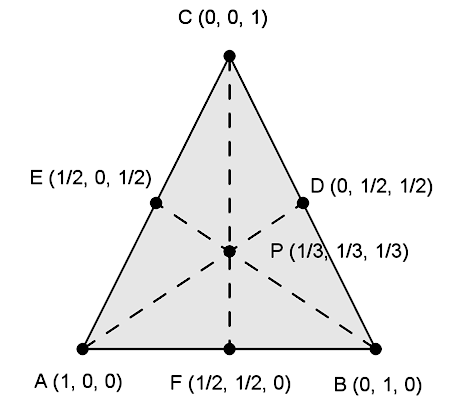
\includegraphics[scale=0.3]{figures/barycentric.png}
    \caption{Barycentric coodrinates of a 2-simplex. Here, the simplex is $s=\langle A,B,C\rangle$ and the triples of numbers next to each point $\alpha\in |s|$ in this triangle correspond to the list of values $(\alpha(A),\alpha(B),\alpha(C))$. The values of $\alpha$ thus represent the proportions in which $A,B,C$ have to be ``mixed'' to get a point inside this geometric realization of the simplex.\label{fig. simplex}}
\end{figure}


In the future we write $|K|=|K|_c$ and call this space the \emph{geometric realization} of $K$. For a simplex $s$ we define the \emph{closed simplex} $|s|\subset |K|$ as $|s|=\{\alpha\in|K|\mid \alpha(e)\neq 0\Rightarrow e\in s\}$ and the \emph{open simplex} as $\langle s\rangle=\{\alpha\in |K|\mid \alpha(e)\neq 0\Leftrightarrow e\in s\}$. The \emph{combinatorial boundary} of $|s|$ is $\partial|s|=|s|\setminus\langle s\rangle$.

\begin{defn}[Standard simplices in $\bbR^k$]
    Let $x_0,\ldots,x_n$ be affinely independent (i.e.\ $\sum_i\alpha_i x_i=0$ and $\sum_i\alpha_i=0$ imply $\alpha_j=0$). Then the simplex spanned by them is \[\langle x_0,\ldots,x_n\rangle=\left\{\sum_i \alpha_i x_i\mid \alpha_i\geq 0,\sum_i \alpha_i=1\right\}.\]
\end{defn}
\begin{defn}
    If $K=(E,S)$ is a simplicial complex and $\{x_e\mid e\in E\}$ a set of points in $\bbR^k$, and if a map
    \[f:|K|\to \bbR^k,\quad \alpha\mapsto \sum_{e\in E}\alpha(e)x_e\]
    is an embedding (say, topological), then $f(|K|)$ is called a simplicial polyhedron in $\bbR^k$ of type $K$, or a polyhedral realization of $K$ in $\bbR^k$.
\end{defn}
\begin{defn}[Triangulation]\index{Triangulation}
    Let $X$ be a topological space. A triangulation of $X$ is a triple $(X,K,f)$ where $K$ is a simplicial complex $K$ such that there is a homeomorphism $f:X\to |K|$.
\end{defn}

It is known that all differentiable manifolds can be triangulated, and the triangulation can be chosen so that on each simplex it is a smooth embedding.

\begin{defn}[Simplicial homology]\index{Homology!simplicial}
    For a simplicial complex $K=(E,S)$ define the group $C^\Delta_p(K)$ of \emph{simplicial $p$-chains} as the free abelian group generated by the set of all $p$-simplices in $K$. That is, elements of $C^\Delta_p(K)$ are formal sums $\sum_{s} c_s s$, where $s$ runs over all $p$-simplices in $K$, and only a finite number of coefficients $c_s\in \bbZ$ are nonzero at once.
    
    Define the \emph{boundary operator}\index{Boundary operator}
    \[\partial:\; C^\Delta_p(K)\to C^\Delta_{p-1}(K),\quad \partial\langle e_0,\ldots,e_p\rangle=\sum_{i=0}^p(-1)^p\langle e_0,\ldots,\wh{e}_i,\ldots,e_p\rangle,\]
    where the hat means skipping a vertex. It is easy to check that $\partial^2=0$, therefore we have the \emph{chain complex}\index{Complex!of simplicial chains}
    \[\cdots\to C^\Delta_2(K)\overset\partial\to C^\Delta_1(K)\overset\partial\to C^\Delta_0(K)\to 0.\]
    The group of $p$-cycles is $Z_p=\ker \restr{\partial}{C^\Delta_p(M)}$ and the group of $p$-boundaries is $B_p=\restr{\im\partial}{C^\Delta_{p+1}(M)}$. The \emph{simplicial homology groups} of $K$ are defined as
    \[H^\Delta_p(K)=Z_p/B_p.\]
\end{defn}

Intuitively, $H^\Delta_p$ detects the ``$p$-dimensional holes'' in the complex, because it consists of cycles that are not boundaries of anything $p+1$-dimensional.

\begin{defn}[Orientations on simplices and complexes]\index{Orientation!on simplicial complexes}
    An orientation on an $n$-simplex $s$ is an ordering of its elements into an $(n+1)$-tuple written as \[s=\langle e_0,\ldots,e_n\rangle.\]
    Orientations are considered to be equivalent if they differ by an even permutation of the vertices, i.e.\ we identify positively reordered tuples with each other. 
    
    In simplicial $p$-chains, sometimes the chain $-s$ is identified with $s$ oriented the opposite way.
    
    An orientation on a complex $K=(E,S)$ is a partial order on $E$ that induces an orientation on each simplex of $K$ (i.e.\ orientations of faces of a simplex can be induced from the orientation of the simplex). Orientations are considered to be equivalent if they induce equivalent orientations on all simplices.
\end{defn}

\begin{comment}
    \begin{samepage}
        \PRLsep
        \begin{center}
            {\red Lecture 21 on 10 May 2019 ended here (but Section \ref{finite dim de rham} was covered in the next lecture)}
        \end{center}
    \end{samepage}
\end{comment}

\begin{example}[Simplicial homology of $\bbS^1$]
    A circle $\bbS^1$ can be triangulated by a regular $n$-gon with vertices  $e_0,\ldots,e_{n-1}$ and oriented simplices $s_i=\langle e_i,e_{i+1}\rangle$, $0\leq i\leq n-1$ with the identification $e_n=e_0$. 
    Clearly 
    \[Z_0=C^\Delta_0=\bbZ^n,\quad C^\Delta_1=\left\{\sum_i c_i s_i \mid c_i\in \bbZ\right\}\cong \bbZ^n,\quad B_1=0.\]
    The chain complex is described by 
    \[\partial\langle e_i,e_{i+1}\rangle=\langle e_i\rangle-\langle e_{i+1}\rangle .\]
    $B_0$ consists of 0-chains $\sum c_i \langle e_i\rangle$ such that $\sum c_i=0$, thus $B_0\cong \bbZ^{n-1}$.
    Finally, $Z_1$ consists of 1-chains $\sum_i c_i s_i$ such that $c_i-c_{i+1}=0$ for all $i$, which means that $Z_1\cong \bbZ$ generated by the cycle $\sum_i s_i$. In the end, we have
    \[H^\Delta_0\cong \bbZ^n/\bbZ^{n-1}\cong \bbZ,\quad H^\Delta_1=Z_1\cong \bbZ. \]
    We notice that the ranks of these homology groups coincide with the dimensions of the corresponding de Rham cohomologies, see Example \ref{de Rham of circle}. We will later prove this as a general fact for all manifolds: the de Rham cohomology is isomorphic to the simplicial homology with real coefficients.
\end{example}


\begin{xca}
    If $K$ is the tetrahedron (with 2-dimensional faces included), i.e.\ a triangulation of $\bbS^2$, compute its homology groups:
    \[H^\Delta_0=\bbZ,\quad H^\Delta_1=0,\quad H^\Delta_2=\bbZ.\]
\end{xca}
\begin{xca}
    Triangulate the M\"obius band as in the figure.
    \begin{center}
        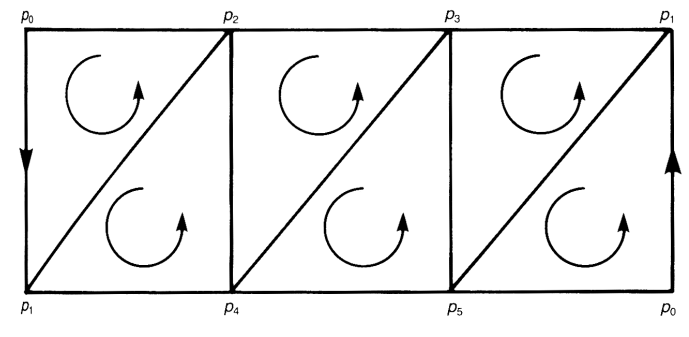
\includegraphics[scale=0.2]{figures/mobius.png}
    \end{center}
    Show that $H^\Delta_2(K)=0$ and $H^\Delta_1(K)=\bbZ$. In fact, the generator of $H^\Delta_1$ is the loop going from the bottom left to the top right corner in the diagram above.
\end{xca}

\begin{xca}
    Triangulate the real projective plane $\bbR P^2$ (which is homeomorphic to a disk whose antipodal boundary points have been identified) as in the figure.
    \begin{center}
        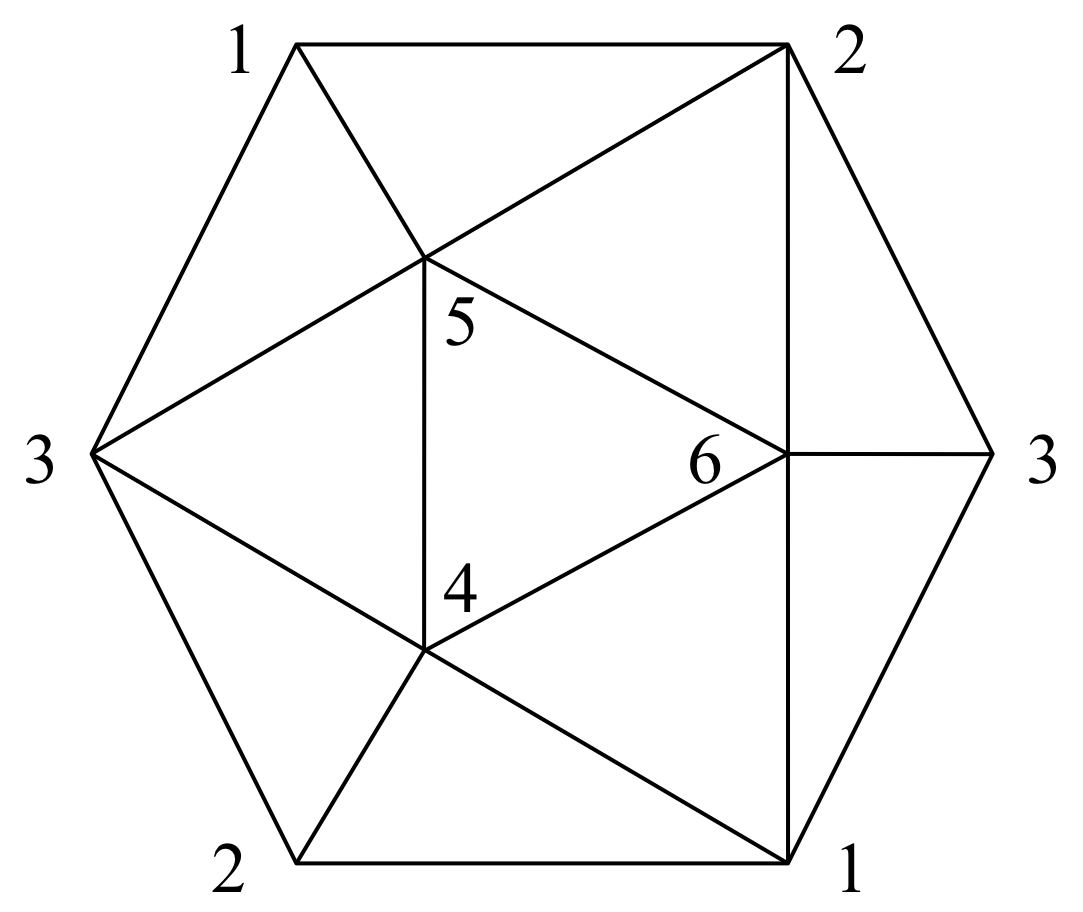
\includegraphics[scale=0.2]{figures/projectiveplane.png}
    \end{center}
    Show that $H^\Delta_2(K)=0$ and $H^\Delta_1(K)=\bbZ_2=\bbZ/2\bbZ$.
\end{xca}
\begin{xca}
    Triangulate the Klein bottle and show that $H^\Delta_1(K)=\bbZ\oplus\bbZ_2$.
\end{xca}

% \begin{defn}[Betti numbers]\index{Betti numbers}
%     Let $K$ be a finite simplicial complex. By the fundamental theorem of finitely generated abelian groups, each homology group of $K$ can be decomposed as
%     \[H_p(K)=\underbrace{\bbZ^{b_p(K)}}_{\text{free part}}\oplus \underbrace{\bbZ_{m_1}\oplus \cdots \oplus \bbZ_{m_k}}_{\text{torsion part}},\]
%     where $b_p(K)\geq 0$ are called \emph{Betti numbers}. 
%     Since the torsion part disappears when tensor multiplied by a field containing the rationals $\bbQ$ (the tensor product is understood to be over the ring $\bbZ$ because abelian groups are $\bbZ$-modules; then, say, $Z_m\otimes \bbQ$ consists of $a\otimes r=ma\otimes (r/m)=0$), we have
%     \[H_p(K)\otimes \bbQ=\bbQ^{b_p(K)}.\]
%     If $K$ is a triangulation of a smooth manifold $M$, then we will also show that $b_p(K)=\dim H_{\rm dR}^p(M)$.
% \end{defn}

% \begin{defn}[Euler characteristic]\index{Euler characteristic}
%     If $K$ is a finite $n$-dimensional simplicial complex, then there are two definitions of the Euler characteristic $\chi(K)$:
%     \begin{itemize}
%         \item $\chi(K)=\sum_{p=0}^n (-1)^p n_p(K)$, where $n_p(K)$ is the number of $p$-simplices in $K$ (``combinatorial Euler characteristic'');
%         \item $\chi(K)=\sum_{i=0}^n (-1)^p b_p(K)$, where $b_p(K)$ are the Betti numbers (``homological Euler characteristic'').
%     \end{itemize}
% \end{defn}

% \begin{thm}[Euler-Poincar\'e]
%     The two definitions of the Euler characteristic for finite simplicial complexes are equivalent. In particular, since the Betti numbers are homotopy invariants (because so is homology itself, which we will show later), so is the Euler characteristic.
% \end{thm}
% \begin{proof}
%     Consider chain groups with rational coefficients (i.e.\ the free parts of the usual groups),
%     \[C_p(K,\bbQ)\coloneqq C_p(K)\otimes\bbQ.\]
%     Now the boundary operator $\partial_p:C_p(K,\bbQ)\to C_{p-1}(K,\bbQ)$ is a linear operator on $\bbQ$-vector spaces and by the rank-nullity theorem
%     \[n_p(K)=\dim C_p(K,\bbQ)=\dim\ker\partial_p+\dim\im\partial_p.\]
%     On the other hand,
%     \[b_p(K)=\dim Z_p(K,\bbQ)/B_p(K,\bbQ)=\dim\ker\partial_p-\dim\im\partial_{p+1}.\]
%     When taking alternating sums of these over $p$, we will get the same answer in both cases.
% \end{proof}




\subsection{Homological algebra II: complexes}

\begin{defn}[(Co)chain complexes]\index{Complex!of chains}\index{Complex!of cochains}
    A chain complex $(\bm{C},d)$ in an abelian category $\calC$ is a sequence  of morphisms 
    \[\cdots\to C_{n+1}\overset{d_{n+1}}\to C_n\overset{d_n}\to C_{n-1}\to\cdots\]
    indexed by $n\in \bbZ$, such that $d_n\circ d_{n+1}=0$.
    
    Similarly, a cochain complex is a sequence
    \[\cdots\to C^{n-1}\overset{d^{n-1}}\to C^n\overset{d^n}\to C^{n+1}\to\cdots\]
    such that $d^{n+1}\circ d^n=0$.
\end{defn}

Note that there is no actual difference between chain and cochain complexes, since simply changing the enumeration $n\mapsto -n$ turns one into the other. Therefore all general results need to be proven only for chain complexes.

\begin{defn}[(Co)cycles, (co)boundaries, (co)homologies of complexes]\index{Homology!of a chain complex}\index{Cohomology!of a cochain complex}
    For a chain complex $(\bm{C},d)$, $n$-cycles, $n$-boundaries, and homologies are defined as 
    \[Z_n(\bm{C},d)=\ker d_n,\quad\quad B_n(\bm{C},d)=\im d_{n+1},\quad\quad H_n(\bm{C},d)=Z_n(\bm{C},d)/B_n(\bm{C},d).\]
    
    Similarly, for a cochain complex $(C^\bullet,d)$, we have cocycles, coboundaries, and cohomologies:
    \[Z^n(C^\bullet,d)=\ker d_n,\quad\quad B^n(C^\bullet,d)=\im d^{n-1},\quad\quad H^n(C^\bullet,d)=Z^n(C^\bullet,d)/B^n(C^\bullet,d).\]
\end{defn}

\begin{defn}[Chain map]
    If $(\bm{B},\delta )$ and $(\bm{C},d)$ are two chain complexes, then a chain map $f:\bm{B}\to \bm{C}$ is a sequence of maps $f_n:B_n\to C_n$ such that $d_n\circ f_n=f_{n-1}\circ \delta_n$, i.e.\ such that the full diagram commutes:
    \[\begin{tikzcd}[every matrix/.append style={name=m},
        execute at end picture={\draw [<-] ([xshift=-8mm,yshift=-10mm]m-1-3.north) arc[start angle=-90,delta angle=-270,radius=0.2cm];
        \draw [<-] ([xshift=-8mm,yshift=-10mm]m-1-4.north) arc[start angle=-90,delta angle=-270,radius=0.2cm];}]
        \cdots\arrow[r] & B_{n+1}\arrow[r]\arrow[d,swap,"f_{n+1}"] & B_{n} \arrow[r]\arrow[d,swap,"f_n"] & B_{n-1}\arrow[d,"f_{n-1}"]\arrow[r] & \cdots \\
       \cdots\arrow[r] & C_{n+1}\arrow[r] & C_n\arrow[r] &C_{n-1} \arrow[r] &\cdots
    \end{tikzcd}\]
    Similarly one defines cochain maps between cochain complexes.
\end{defn}

\begin{prop}
    All chain complexes in an abelian category $\calC$ with chain maps between them comprise an abelian category called $\mathsf{Comp}(\calC)$.
\end{prop}
\begin{proof}
    By the Freyd-Mitchell theorem, we only need to prove this for $\calC=R\text{-}\mathsf{Mod}$. For such a category it is obvious what the structure of an abelian category on complexes is: the zero object is the zero complex; direct sums are defined by summing in each degree; the kernel and cokernel of $f$ are the complexes consisting of $\ker f_n$ and $\coker f_n$; images and coimages coincide because they do so in $\calC$.
\end{proof}

\begin{defn}[Positive complexes]
    A chain complex $\bm{C}$ is called positive if $C_n=0,n<0$. All positive complexes form the full subcategory $\mathsf{Comp}_{\geq 0} (\calC)$ of $\mathsf{Comp}(\calC)$:
    \[\cdots\to C_n\to C_{n-1}\to\cdots\to \to C_1\to C_0\to 0.\]
    
    A negative chain complex
    \[0\to C_0\to C_{-1}\to \cdots \to C_{-n}\to C_{-n-1}\to\cdots\]
    is identified with a positive cochain complex 
    \[0\to C^0\to C^{1}\to \cdots \to C^{n}\to C^{n+1}\to\cdots\]
    by setting $C^n=C_{-n}$ and $d^n=d_{-n}$.
\end{defn}

\begin{prop}
    If $\calC$ is an abelian category, then the $n$-th homology $H_n:\mathsf{Comp}(\calC)\to \calC$ is an additive (covariant) functor for all $n\in \bbZ$.
\end{prop}
\begin{proof}
    Given a chain map $f:\bm{A}t\to \bm{B}$, we need to construct a morphism $H_n(f):H_n(\bm{A})\to H_n(\bm{B})$. Since $H_n(\bm{A})=Z_n(\bm{A})/B_n(\bm{A})$, we can try to take a $z$ such that
    \[f_n:Z_n(\bm{A})\to B_n,\quad z\mapsto f_n(z)\]
    and define
    \[H_n(f):H_n(\bm{A})\to H_n(\bm{B}),\quad [z]\to \left[f_n(z)\right],\]
    where equivalence classes are taken w.r.t.\ to the quotients by $B_n(\bm{A})$ and $B_n(\bm{B})$ respectively.
    
    First we need to check that $f_n(z)\in Z_n(\bm{B})$. We will use the same symbol $d_n$ for morphisms in both complexes. By the definition of a chain map, $d_n(f_n(z))=f_{n-1}(d_n(z))=0$ since $z\in B_n(\bm{A})$.
    
    Next we need to check correctness, i.e.\ independence of $H_n(f)([z])$ of the choice of representative. Let $z,z'\in Z_n(\bm{A}):[z]=[z']\Leftrightarrow z-z'\in B_n(\bm{A})$, then
    \[\exists y\in A_{n+1}: d_{n+1}(y)=z-z'\implies d_{n+1}(f_{n+1}(y))=f_n(z)-f_n(z'),\]
    which means that $f_n(z)-f_n(z')$ is a boundary, proving what we wanted.
    
    To check functoriality, say we have two chain maps
    \[\bm{A}\overset f\to \bm{B}\overset g\to \bm{C}.\]
    We need to show the commutativity of the triangle
    \[
    \begin{tikzcd}
        H_n(\bm{A}) \arrow[rr,"H_n(f)"]\arrow[dr,swap,"H_n(g\circ f)"]&& H_n(\bm{B})\arrow[dl,"H_n(g)"]\\
        & H_n(\bm{C}) &
    \end{tikzcd}
    \]
    We have 
    \begin{multline}
        H_n(g\circ f)([z])=\left[(g\circ f)_n(z)\right]=\left[g_n\circ f_n(z)\right]=H_n(g)\left(\left[f_n(z)\right]\right)=\\=H_n(g)\left(H_n(f)[z]\right)=H_n(g)H_n(f)([z]).
    \end{multline}
    
    Finally, additivity is trivial since $f_n$ are homomorphisms:
    \[H_n(f+f')=H_n(f)+H_n(g').\]
\end{proof}

\begin{rem}
    On cochain complexes, this functor is of course contravariant.
\end{rem}

From now on we write
\[f_\ast=H_n(f),\quad\quad g^\ast=H^n(g)\]
for the descendants of maps in (co)homology.

\begin{lem}
    Exact additive covariant functors preserve homology: $H_\ast(F(\bm{C}))\cong F(H_\ast(\bm{C}))$.
\end{lem}
\begin{proof}
    This follows from the fact that exact additive functors preserve kernels and quotients (and all functors preserve images).
\end{proof}

\begin{prop}
    The direct limit of the homology groups of a directed system of chain complexes $\bm{C}^i$ is the homology group  of the direct limit:
    \[\colimit_i H_n(\bm{C}^i)\cong H_n(\colimit_i \bm{C}^i).\]
\end{prop}
\begin{proof}
    This follows immediately from the preceding Lemma and the fact that direct limits preserve exactness in abelian categories (Proposition~\ref{prop direct limits preserve exactness}).
\end{proof}
\begin{rem}
    Note that the analogous statement for homotopy groups $\pi_n$ was proven by us only for sequences of $CW$ subcomplexes (Corollary~\ref{cor direct limit of pi_n for CW}) and does not hold in general even for $\pi_1$.
\end{rem}



\begin{thm}[Connecting homomorphism lemma]\label{connecting hom in homology}
    Let 
    \[0\to \bm{A}\overset i\to \bm{B}\overset\pi\to \bm{C}\to 0 \]
    be a short exact sequence of chain complexes. Then for each $n$ there is a \emph{connecting homomorphism}
    \[\delta=\delta_n:H_n(\bm{C})\to H_{n-1}(\bm{A}),\quad [z]\to \left[i_{n-1}^{-1} d_n\pi_n^{-1}(z)\right].\]
\end{thm}
\begin{proof}
    Several checks need to be done. First, why does $d_n\pi_n^{-1}(z)\in\im i_{n-1}$? Let $y:\pi_n(y)=z$, then $d_n(y)\in B_{n-1}$. Since $z\in Z_n(\bm{C})$ we have $\pi_{n-1}(d_n(y))=d_n(\pi_n(y))=d_n(z)=0$. Therefore $\exists ! x\in A_{n-1}:i_{n-1}(x)=d_n(y)$, and we have a well defined map
    \[z\mapsto x.\]
    
    Next, we need to verify that $d_{n-1}(x)=0$ and the class $[x]\in H_{n-1}(\bm{A})$ is independent of the choice of $y$.
    Moreover, one needs to check that if $[z]=[z']$, then $[x]=[x']$. Lastly, we need to check that $\delta$ is a homomorphism. These checks are left as an exercise.
\end{proof}

\begin{thm}[Zig-zag lemma/Long exact sequence in homology]\label{thm long exact seq in homology}
    For any short exact sequence of complexes 
    \[0\to \bm{A}\overset i\to \bm{B}\overset\pi\to \bm{C}\to 0 ,\]
    the induced sequence in homology
    \[\cdots \to H_{n+1}(\bm{C})\overset{\delta_{n+1}}\to H_n(\bm{A})\overset{i_\ast}\to H_n(\bm{B})\overset{\pi_\ast}\to H_n(\bm{C})\overset{\delta_n}\to H_{n-1}(\bm{A})\to \cdots \]
    is exact.
\end{thm}
\begin{proof}
    It is easy to see that for any complex $\bm{C}$ the two \emph{``fundamental sequences''}
    \[0\to Z_n(\bm{C})\to C_n\overset{d_n}\to B_{n-1}(\bm{C})\to 0,\]
    \[0\to B_n(\bm{C})\to Z_n(\bm{C})\to H_n(\bm{C})\to 0\]
    are short exact.
    This one is also obviously exact:
    \[0\to B_n(\bm{C})\to C_n\to C_n/B_n(\bm{C})\to 0.\]
    Using the exactness of the first sequence, we also have the exactness of this one:
    \[0\to H_n(\bm{C})\to C_n/B_n(\bm{C})\to \underbrace{B_{n-1}(\bm{C})}_{\cong C_n/Z_n(\bm{C})}\to 0.\]
    
    Putting it all together, we conclude the exactness of this sequence:
    \[0\to H_n(\bm{C})\to C_n/B_n(\bm{C})\to Z_{n-1}(\bm{C})\to H_{n-1}(\bm{C})\to 0.\]
    Now let us use this sequence for the columns of one large diagram:
    \[\begin{tikzcd}
        && 0\ar{d}& 0\ar{d} &0\ar{d} &&\\
        & & H_n(\bm{A}) \ar{r} \ar{d} & H_n(\bm{B})\ar{r} \ar{d} &  H_n(\bm{C}) \ar{d}   %\arrow[ddll,"\delta",rounded corners
        & & \\
        &  &  A_n/B_n(\bm{A}) \ar{r} & B_n/B_n(\bm{B}) \ar{r} \ar{dd} &  C_n/B_n(\bm{C})\ar{r}\ar{dd} & 0 &  ~\\[-10pt]
        & & &  ~ & & \ar[r, phantom, ""{coordinate, name=Y}] & ~\\[-10pt]
        ~&  \ar[l, phantom, ""{coordinate, name=Z}] 0 \ar{r} &  Z_{n-1}(\bm{A}) \ar[uu,leftarrow,crossing over]\ar{r} \ar{d} &  Z_{n-1}(\bm{B}) \ar{r} \ar{d} &  Z_{n-1}(\bm{C}) \ar{d} & &  \\
              & &  \ar[from=uuuurr, "\delta_n", dashed,crossing over, rounded corners,
                      to path=
                              { -- ([xshift=2ex]\tikztostart.east)
                              -| (Y) [near end]\tikztonodes
                              -| (Z) [near end]\tikztonodes
                              |- ([xshift=-2ex]\tikztotarget.west)
                               -- (\tikztotarget)}
                    ] H_{n-1}(\bm{A})\ar{r}\ar{d}
               &  H_{n-1}(\bm{B}) \ar{r}\ar{d}
               &  H_{n-1}(\bm{C})\ar{d}
               & 
               & \\
        && 0& 0 &0 &&\\
    \end{tikzcd}\]
    The exactness of the rows can be checked directly using the exactness of $\bm{A}\to \bm{B}\to\bm{C}$. Then this is in fact exactly the type of diagram for which we can apply the Snake Lemma \ref{snake lemma} and establish the existence of $\delta_n$. It only remains to check that the construction of $\delta_n$ in the Snake Lemma exactly coincides with the one in Proposition \ref{connecting hom in homology}.
\end{proof}
\begin{cor}
    The Snake lemma is equivalent to the Zig-zag lemma.
\end{cor}
\begin{proof}
     The proof of Theorem \ref{thm long exact seq in homology} shows that the Snake Lemma implies the long exact sequence in homology. The converse also trivially holds since we can apply the Zig-zag lemma to a short exact sequence of complexes concentrated in just two degrees of the form $0\to \ker\pi \to \im\pi \to 0$ (let the two other complexes have $\rho $ and $\sigma$ instead of $\pi$) and obtain the long exact sequence of homologies, which reads
    \[0\to \ker\pi \to \ker\rho\to \ker\sigma\to \coker\pi\to \coker\rho\to\coker\sigma\to 0, \]
    which is exactly the Snake Lemma \ref{snake lemma}.
\end{proof}

\begin{comment}
    \begin{samepage}
        \PRLsep
        \begin{center}
            {\red Lecture 22 on 17 May 2019 ended here (included Section \ref{finite dim de rham})}
        \end{center}
    \end{samepage}
\end{comment}


\begin{prop}[Naturality of the connecting homomorphism\tablefootnote{Tape worm lemma?}]\label{naturality of connecting hom}
    Given a commutative diagram with exact rows in the category $\mathsf{Comp}(\calC)$
    \[\begin{tikzcd}
        0\arrow[r] & \bm{A}\arrow[r,"i"]\arrow[d,swap,"f"] & \bm{B} \arrow[r,"p"]\arrow[d,swap,"g"] & \bm{C}\arrow[d,"h"]\arrow[r] & 0 \\
       0\arrow[r] & \bm{A}'\arrow[r,"j"] & \bm{B}'\arrow[r,"q"] &\bm{C}' \arrow[r] &0
    \end{tikzcd}\]
    there is a commutative diagram in $\calC$ with exact rows
    \[\begin{tikzcd}
        ~\arrow[r]& H_n(\bm{A})\arrow[r,"i_\ast"]\arrow[d,"f_\ast"] & H_n(\bm{B}) \arrow[r,"p_\ast"]\arrow[d,"g_\ast"] & H_n(\bm{C})\arrow[d,"h_\ast"]\arrow[r,"\delta"] & H_{n-1}(\bm{A})\arrow[d,"f_\ast"]\arrow[r]&~ \\
       ~\arrow[r] & H_n(\bm{A}')\arrow[r,"j_\ast"] & H_n(\bm{B}')\arrow[r,"q_\ast"] &H_n(\bm{C}') \arrow[r,"\delta'"] &H_{n-1}(\bm{A}')\arrow[r]&~ 
    \end{tikzcd}\]
    In other words, morphisms between exact sequences of complexes naturally induce morphisms between the exact sequences in homology, i.e.\ the connecting homomorphism $\delta$ is natural w.r.t.\ such morphisms.
\end{prop}
\begin{proof}
     The exactness of the rows is the content of the theorem about the long exact sequence. The commutativity of the first two squares follows from the functoriality of $H_n$. Checking the commutativity of the square $\delta'\circ h_\ast=f_\ast\circ \delta$ requires expanding the first commutative diagram in $\mathsf{Comp}(\calC)$ into a 3-dimensional diagram in $\calC$.
     \[
     \begin{tikzcd}[column sep={35,between origins}]
        &
        0 
        \ar{rr}
        & &
        A_n
        \ar{dl}[swap, sloped, near start]{d}
        \ar{rr}{i}
        \ar[]{dd}[near start]{f_\ast}
        & & B_n
        \ar{dd}[near start]{g_\ast}
        \ar{rr}{p}
        \ar{dl}[swap, sloped, near start]{d}
        & & C_n
        \ar{dd}[near start]{h_\ast}
        \ar{dl}[swap, sloped, near start]{d}
        \ar{rr}
        & &
        0
        \\
        0
        \ar{rr}
        & &
        A_{n-1}
        \ar[crossing over]{rr}[near end]{i}
        & & B_{n-1}
        \ar[crossing over]{rr}[near end]{p}
        & & C_{n-1}
        \ar[crossing over]{rr}
        & &
        0
        \\
        &
        0
        \ar{rr}
        & &
        A_n'
        \ar[near start]{rr}{j}
        \ar[sloped, swap]{dl}{d}
        & & B_n'
        \ar[near start]{rr}{q}
        \ar[sloped, swap]{dl}{d}
        & & C_n'
        \ar[sloped, swap]{dl}{d}
        \ar{rr}
        & &
        0
        \\
        0
        \ar{rr}
        & &
        A_{n-1}'
        \ar{rr}{j}
        \ar[crossing over, leftarrow, near start]{uu}{f_\ast}
        & & B_{n-1}'
        \ar{rr}{q}
        \ar[crossing over, leftarrow, near start]{uu}{g_\ast}
        & & C_n'
        \ar[crossing over, leftarrow, near start]{uu}{h_\ast}
        \ar{rr}
        & &
        0
        \end{tikzcd}
     \]
     Taking $[c]\in H_n(\bm{C})$, we must show that $f_\ast\delta [c]=\delta ' h_\ast [c]$. Let $b\in B_n$ be such that $p(b)=c$. Then $\delta [c]=[a]$, where $i(a)=d(b)$. Hence $f_\ast \delta [c]=[f(a)]$. 
     
     On the other hand, since $h$ is a chain map, $q(g(b))=h(p(b))=h(c)$. Hence we can use $g(b)$ as the pre-image of $h(c)$ in $B_n'$, so by construction of the connecting homomorphism, $\delta '[h(c)]=[a']$ where $j(a')=d(g(b))$. But $j(f(a))=g(i(a))=g(d(b))=d(g(b))=j(a')$ and so $f(a)=a'$ because $j$ is injective. Therefore $\delta'h_\ast [c]=[a']=[f(a)]$, which coincides with the l.h.s.\ computed above.
\end{proof}

Naturality is instrumental in many arguments involving long exact sequences because it means that we can apply sequences of chain maps to long exact sequences and preserve the commutativity of diagrams.

\begin{prop}[Algebraic Mayer-Vietoris sequence]\label{prop algebraic MV}
    If in the setting of Theorem \ref{naturality of connecting hom}, $h_\ast$ is also an isomorphism in homology, then one has the long exact sequence
    \[\cdots \to H_{n+1}(\bm{B}')\overset\Delta\to H_n(\bm{A})\overset{(f_\ast,i_\ast)}\longrightarrow H_n(\bm{A}')\oplus H_n(\bm{B})\overset{j_\ast- g_\ast}\longrightarrow H_n(\bm{B}')\overset{\Delta}\to H_{n-1}(\bm{A})\to \cdots\]
    where $\Delta=\delta \circ h_\ast^{-1}\circ q_\ast$.
\end{prop}
\begin{proof}
     This is an exercise in diagram chasing.
\end{proof}

The relation of this Proposition to the \gls{mv} sequence in de Rham cohomology will become clear when we get to relative (co)homology and the excision property. The isomorphism $h_\ast$ in question is $H_n(U,U\cap V)\cong H_n(M,V)$ for $M=U\cup V$. A rough visualization of $H_n(X,Y)$ with $Y\subset X$ is the homology of the space obtained from $X$ by contracting $Y$ into one point. Then it is clear that contracting $V$ inside $M$ has the ``same'' result as contracting $U\cap V$ inside $U$. 


\begin{defn}[Maps of degree $p$]
    Let $\bm{C}$ and $\bm{D}$ be two chain complexes in $\calC$. A map of degree $p$ between them, denoted $s:\bm{C}\to \bm{D}$, is a collection of maps $s_n:C_n\to D_{n+p}$. Note that no commutativity is required here!
\end{defn}


Now that we know that $H_n$ is a functor, it is natural to ask how much $H_n(f)$ actually depends on $f$. It turns out that $H_n(f)$ is invariant under homotopies of $f$ defined in the following categorical sense.


\begin{defn}
    Let $f,g:\bm{B}\to \bm{C}$ be two chain maps. They are called homotopic ($f\sim g$) if there is a map of degree $+1$ denoted $s:\bm{B}\to \bm{C}$ such that 
    \[\forall n,\quad f_n-g_n=d_{n+1}s_n+s_{n-1}d_n.\]
    (As usual, we use $d_n$ to denote the differentials in all complexes at once).
    This can be visualized by the following \emph{non-commutative} diagram:
     \[\begin{tikzcd}
        \cdots\ar[r] & B_{n+1}\ar[r]\ar[dd,swap, xshift=-.75ex,"f_{n+1}"]\ar[dd,xshift=.75ex,"g_{n+1}"] & B_{n} \arrow[r]\ar[dd,swap,xshift=-.75ex,"f_n"]\ar[dd,xshift=.75ex,"g_n"]\ar[ddl,sloped, near start,"s_n"] & B_{n-1}\ar[dd,swap,xshift=-.75ex,"f_{n-1}"]\ar[dd,xshift=.75ex,"g_{n-1}"]\ar[r]\ar[ddl, near start,sloped,"s_{n-1}"] & \cdots \\
        &&&&\\
       \cdots\ar[r] & C_{n+1}\ar[r] & C_n\ar[r] &C_{n-1} \ar[r] &\cdots
    \end{tikzcd}\]
\end{defn}

\begin{thm}
    Homotopic chain maps induce the same morphism in homology.
\end{thm}
\begin{proof}
     Let $s:\bm{B}\to\bm{C}$ be the homotopy. If $z$ is an $n$-cycle, dropping subscripts, $d z=0$, then
     \[f(z)-g(z)=d(s(z))+s(d(z))=d(s(z)),\]
     i.e.\ $f(z)-g(z)\in B_n(\bm{C})$ and $f_\ast=g_\ast$.
\end{proof}

\begin{defn}[Acyclic, contractible complexes]\index{Acyclic complex}\index{Contractible complex}
    A complex is called acyclic if all its (co)homologies are trivial. A complex $\bm{C}$ is called contractible if there exists a homotopy $1_{\bm{C}}\sim 0_{\bm{C}}$. 
    All contractible complexes are acyclic since contractibility implies $1_{H_n(\bm{C})}=0_{H_n(\bm{C})}$.
\end{defn}

\begin{defn}[Quasi-isomorphisms]\index{Quasi-isomorphism}
    Two complexes $\bm{A},\bm{B}$ are called quasi-isomorphic (or \emph{weakly equivalent}) if there is a chain map $f:\bm{A}\to \bm{B}$ such that $f_\ast=H_n(f):H_n(\bm{A})\to H_n(\bm{B})$ is an isomorphism for all $n$.
\end{defn}

\begin{defn}[Homotopy equivalence]\index{Homotopy equivalence}
    Two complexes $\bm{A},\bm{B}$ are called homotopy equivalent if there are two chain maps $f:\bm{A}\to \bm{B}$ and $g:\bm{B}\to\bm{A}$ such that
    \[f\circ g\sim 1_{\bm{B}},\quad g\circ f\sim 1_{\bm{A}}.\]
    Clearly homotopy equivalent complexes are quasi-isomorphic.
\end{defn}


\begin{xca}\label{Lie derivative homotopy operator}
    Check that a Lie derivative $\Lie_X$ is a cochain map on the de Rham complex. Furthermore, show that applying a Lie derivative $\Lie_X$ to a differential form doesn't change its class in de Rham cohomology. For this, find the homotopy operator between $\Lie_X$ and the zero morphism.
\end{xca}







\subsection{Singular homology}

de Rham cohomology is defined only for smooth manifolds, and simplicial homology is defined only for triangulable spaces. The type of homology we define now works for all topological spaces, but proving its properties for nicer spaces (like manifolds) requires extra work. The idea is, instead of trying to break up our topological space into simplices, to study the set of all continuous maps from simplices to our space.

\begin{defn}[Singular simplices]\index{Simplex!singular}
    We denote by $\Delta^n$ the standard $n$-simplex $\Delta^n=\{\sum_{i=0}^{n} \alpha_i e_i\mid \sum_i\alpha_i=1\}$, where $\{e_i\}_{i=0}^{n}$ is the standard basis in $\bbR^{n+1}$. Let $X$ be a topological space. A singular $n$-simplex in $X$ is a continuous map $\sigma\in C(\Delta^n, X)$ (no other constraints, hence ``singular''). The group $C_n(X)$ of singular $n$-chains is the free abelian group generated by the set $C(\Delta^n,X)$. Sometimes we will write $C^{\text{sing}}_n(X)$ to distinguish from other kinds of chain groups.
\end{defn}
\begin{defn}[Singular homology]\index{Homology!singular}
    The boundary map $\partial_n:C_n(X)\to C_{n-1}(X)$ is defined as before:
    \[\partial_n\sigma=\sum_i (-1)^i\restr{\sigma}{\langle e_0,\ldots,\wh{e}_i,\ldots,e_n\rangle},\]
    where we implicitly identify the faces of $\Delta^n$ with $\Delta^{n-1}$ while preserving the order of vertices, so that $\restr{\sigma}{\langle e_0,\ldots,\wh{e}_i,\ldots,e_n\rangle}$ is a singular $(n-1)$-simplex.
    
    Singular homology groups are defined as
    \[H_n(X)=\ker\partial_n/\im\partial_{n+1}.\]
\end{defn}

Unlike with simplicial homology, here it is immediately obvious that homeomorphic spaces have isomorphic singular homologies. The price we pay for this is that the rank of $C^{\text{sing}}_n(X)$ is uncountably large, so it is not clear at a glance whether singular homologies of spaces that have finitely generated simplicial homologies are also finitely generated. 

\begin{prop}
    If $X$ consists of $l$ path-connected components, then $H_0(X)\cong \bbZ^l$.
\end{prop}
\begin{proof}
     It suffices to prove this for $l=1$, i.e.\ a path-connected $X$. We have $H_0(X)=C_0(X)/\im\partial_1$. A singular 0-chain in $X$ is just a finite sum $\sum_i n_i p_i$ where $p_i$ are points in $X$ and $n_i\in\bbZ$. Define the homomorphism $\epsilon:C_0(X)\to \bbZ$, called the \emph{augmentation map}\index{Augmentation map}, by
     \[\epsilon\left(\sum_i n_i p_i\right)=\sum_i n_i.\]
     It is surjective as long as $X\neq\varnothing$. The claim is that $\ker\epsilon\cong\im\partial_1$ if $X$ is path-connected, so $\epsilon $ induces an isomorphism $H_0(X)\cong \bbZ$.
     
     First, it is clear by definition of $\partial$ that $\im\partial_1\subset\ker\epsilon$. For the reverse inclusion, suppose $\epsilon(\sum_i n_i p_i)=0$. Choose a path $\gamma_i$ connecting a base point $x_0$ to $p_i$. We can view $\gamma_i$ as a singular 1-simplex and have $\partial\gamma_i=p_i-x_0$. Hence $\partial(\sum_i n_i\gamma_i)=\sum_i n_i p_i$ since $\sum_i n_i=0$. Therefore $\sum n_i p_i$ is a boundary, which shows $\ker\epsilon\subset\im\partial_1$.
\end{proof}

\begin{prop}
    If $X$ consists of a single point, then $H_n(X)=0$ for $n>0$ and $H_0(X)\cong \bbZ$.
\end{prop}
\begin{proof}
     In this case there is a unique singular $n$-simplex $\sigma_n$ for each $n$ and 
     \[\partial\sigma_n=\sum_{i=0}^n(-1)^i\sigma_{n-1}=\begin{cases}
     0,& n\text{ odd},\\
     \sigma_{n-1},& n\text{ even}.
     \end{cases}\]
     This the singular chain complex reads
     \[\cdots\to \bbZ\overset\cong\to \bbZ\overset 0\to \bbZ\overset\cong\to\bbZ\overset 0\to\bbZ\to 0.\]
     The homology of this complex is trivial except for $H_0\cong \bbZ $.
\end{proof}

Sometimes it is very helpful to work with a slightly modified homology that vanishes entirely for a point. The following definition achieves this.

\begin{defn}[Reduced homology]\index{Homology!reduced}
    The reduced homology groups $\wt{H}_n(X)$ are the homology groups of the \emph{augmented chain complex}
    \[\cdots C_1(X)\overset{\partial_1}\to C_0(X)\overset{\epsilon}\to \bbZ\to 0.\]
\end{defn}

The reduced homology of a point is trivial in all degrees. Also $H_n(X)\cong \wt{H}_n(X)$ for all $n>0$ and $H_0(X)=\wt{H}_0(X)\oplus \bbZ$ since $\epsilon$ induces a map $H_0(X)\to \bbZ$ with kernel $\wt{H}_0(X)$.




\subsection{Homotopy invariance}

Here we show that singular homology is homotopy invariant.

\begin{figure}[tp]
    \begin{center}
        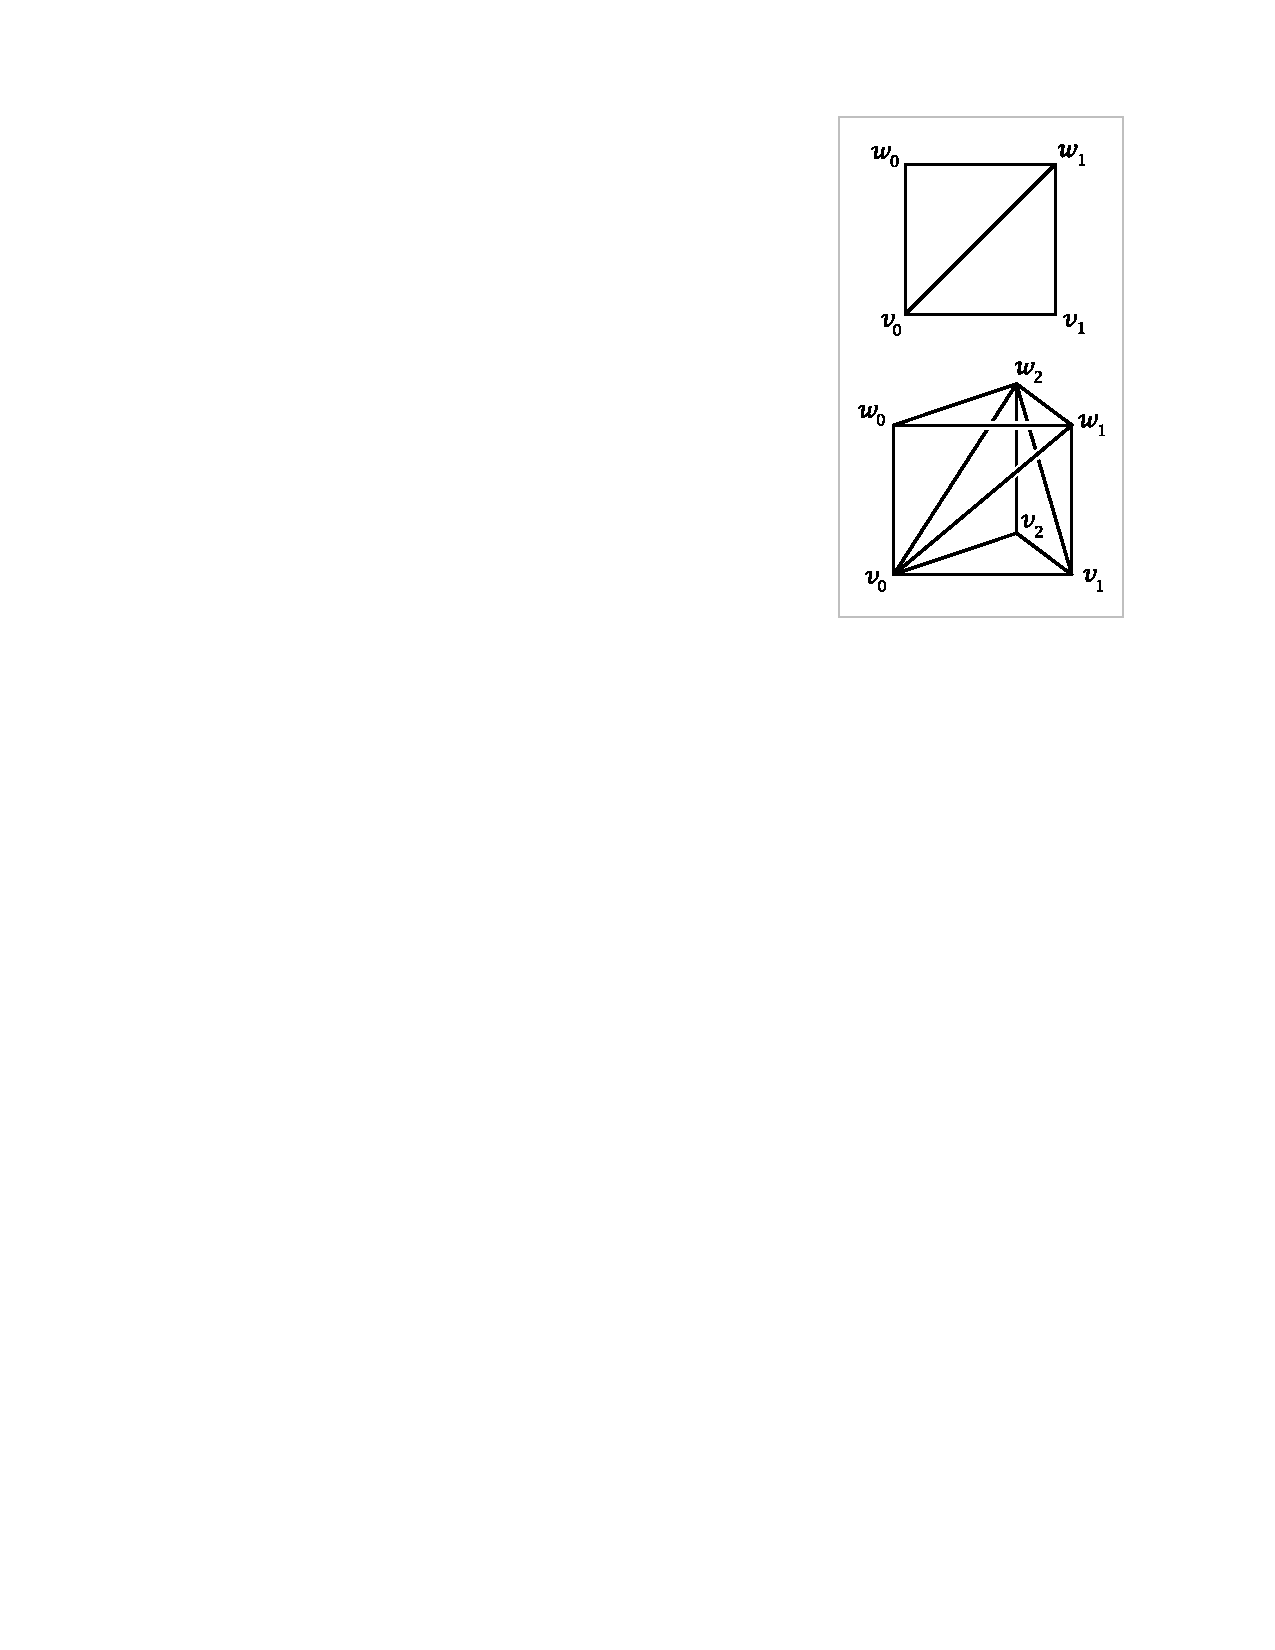
\includegraphics[width=0.2\textwidth]{figures/prism.pdf}
    \end{center}
    \caption{Triangulation of a prism, see Proposition~\ref{thm 2.10 Hatcher}.\label{Prism fig}}
\end{figure}
\begin{prop}[{{\cite[Thm. 2.10]{Hatcher}}}]\label{thm 2.10 Hatcher}
    If two maps $f,g\in C(X,Y)$ between topological spaces $X,Y$ are homotopic, then they induce the same homomorphism in homology
    \[f_\ast=g_\ast :H_n(X)\to H_n(Y)\]
    for all $n$. In particular, homotopy equivalent spaces have isomorphic homology groups.
\end{prop}
\begin{proof}
     The key is learning to subdivide the prism $\Delta^n\times I$ (where $I=[0,1]$) into simplices. If $\langle v_0,\ldots,v_n\rangle$ is the copy of $\Delta^n$ at the bottom of the prism and $\langle w_0,\ldots,w_n\rangle$ is the one at the top, then it is easy to check that the prism is triangulated by the $(n+1)$-simplices $\langle v_0,\ldots,v_i,w_i,\ldots,w_n\rangle$, each intersecting the next in an $n$-simplex face. The cases $n=1,2$ are shown in figure~\ref{Prism fig}.
     
     Given a homotopy $F:X\times I\to Y$ from $f$ to $g$ and a singular simplex $\sigma:\Delta^n\to X$, we form the composition $F\circ(\sigma\times \id):\Delta^n\times I\to X\times I\to Y$. Using this, we define the \emph{prism operators}
     \[P:C_n(X)\to C_{n+1}(Y),\quad P(\sigma)=\sum_i(-1)^i F\circ (\sigma\times\id)\langle x_0,\ldots,v_i,w_i,\ldots,w_n\rangle.\]
     We claim that $P$ is a homotopy operator between these two chain complexes, namely
     \[g_\ast-f_\ast=\partial P+P\partial.\]
     The geometric meaning of $\partial P=g_\ast-f_\ast-P\partial$ is that the boundary of the prism equals its top $\Delta^n\times\{1\}$, minus its bottom $\Delta^n\times\{0\}$, and plus the sides $\partial\Delta^n\times I$ (compare this with Cartan's magic formula and its cohomological meaning, which is nothing but a dual to this geometric statement, see Exercise~\ref{Lie derivative homotopy operator}).
     
     The verification of this identity follows easily by direct expansion and use of the definition of the homotopy $F$ and $g\circ\sigma=g_\ast(\sigma)$ (see \cite[Thm.~2.10]{Hatcher} for full details).
\end{proof}
\begin{cor}
    If $X$ is contractible, then $\wt{H}_n(X)=0$ for any $n$.
\end{cor}


Continuous maps induce homomorphisms in reduced homology as well since the augmentation map $\epsilon$ commutes with $f_\ast$. Then the same theorem holds for reduced homologies with the same proof.




\subsection{Relative homology and excision}

Relative homology generalizes the idea behind the \gls{mv} sequence in de Rham cohomology. Given a subset $A\subset X$ in a topological space, we ask how similar the groups $H_n(X/A)$ and $H_n(X)/H_n(A)$ are. The difference, in a sense, is measured by the relative homology.

\begin{defn}
    Let $X$ be a topological space and $A\subset X$ a topological subspace (i.e.\ a subset with the induced subset topology). The group of singular chains $C_n(A)$ can be treated as a subgroup of $C_n(X)$. Define the relative singular chain groups as $C_n(X,A)=C_n(X)/C_n(A)$. The boundary operator $\partial$ descends to these groups because $\partial(C_n(A))\subset C_{n-1}(A)$. The homology of the resulting chain complex is called the relative homology of the pair $(X,A)$.
\end{defn}

Relative homology is a covariant functor on the category of topological pairs, $H_n:\mathsf{TopPair}\to \mathsf{Ab}$.

\begin{prop}[Exact sequence of a pair]\label{exact seq of a pair}
    The exact sequence of relative chain groups
    \[0\to C_\bullet(A)\to C_\bullet (X)\to C_\bullet(X,A)\to 0 \]
    induces a long exact sequence in relative homology
    \[\cdots \to H_n(A)\to H_n(X)\to H_n(X,A)\to H_{n-1}(A)\to H_{n-1}(X)\to H_{n-1}(X,A)\to \cdots\]
\end{prop}
\begin{proof}
     The first exact sequence is the definition of relative homology and the second one is an application of the Zig-zag lemma.
\end{proof}

The same sequence exists in reduced homology. This exact sequence has a natural geometric interpretation: elements of $H_n(X,A)$ can be thought of as $n$-chains in $X$ that differ from an actual cycle in $X$ only by a chain in $A$, and the connecting homomorphism maps such a cycle into an $(n-1)$-cycle in $A$ by simply computing the boundary.

\begin{cor}
    \begin{enumerate}
        \item $H_n(X,
        \{x_0\})\cong\wt{H}_n(X)$ for all $n$.
        \item If $A$ is contractible, then $H_n(X,A)\cong \wt{H}_n(X)$ for all $n$;
        \item if $X$ is contractible, then $H_{n+1}(X,A)\cong \wt{H}_n(A)$ for all $n$.
    \end{enumerate}
\end{cor}

\begin{example}[Homology of a bouquet of circles]
    Consider $X=\bbR$ and $A\subset \bbR$ a finite subset of size $(k+1)$. Then $X/A$ is homotopy equivalent to a wedge sum of $k$ circles (a.k.a.\ a bouquet of circles). We will later show that $H_1(X,A)\cong \wt{H}_1(X/A)= H_1(X/A)$, so we have $H_1(\bigvee_{i=1}^{k}\bbS^1)=\wt{H}_0(A)=\bbZ^{k}$. We also see that all higher homologies of the bouquet vanish. Another way to obtain this result will be from the Hurewicz theorem.
\end{example}



\begin{prop}[Exact sequence of a triple]\label{exact sequence of a triple}
    For a triple $(X,A,B)$ where $B\subset A\subset X$, the exact sequence of relative chain complexes
    \[0\to C_\bullet(A,B)\to C_\bullet (X,B)\to C_\bullet(X,A)\to 0 \]
    induces a long exact sequence in relative homology
    \[\scriptstyle
    \cdots \to H_n(A,B)\to H_n(X,B)\to H_n(X,A)\to H_{n-1}(A,B)\to H_{n-1}(X,B)\to H_{n-1}(X,A)\to \cdots
    \]
\end{prop}
\begin{proof}
     Exercise.
\end{proof}


\begin{prop}[Homotopy property for relative homology]
    If two maps $f,g:(X,A)\to (Y,B)$ in the category of topological pairs are homotopic also through maps of pairs, then they induce the same homomorphism $f_\ast=g_\ast:H_n(X,A)\to H_n(Y,B)$.
\end{prop}
\begin{proof}
     The prism operator constructed in the proof of the homotopy property induces a relative prism operator $P:C_n(X,A)\to C_{n+1}(Y,B)$. Since we are passing to quotient groups, the formula $\partial P+P\partial=g_\ast-f_\ast$ still holds and $f_\ast,g_\ast$ are chain homotopic on relative chain groups. 
\end{proof}


For a space $X$, let $\calU=\{U_\alpha\}_\alpha$ be a collection of subspaces of $X$ whose interiors cover $X$ and let $C_n^\calU(X)$ be the subgroup of $C_n(X)$ generated by simplices whose images lie inside one of the sets in the cover. The boundary operator $\partial$ maps $C^\calU_n(X)$ to $C^\calU_{n-1}(X)$ and therefore we have a chain complex $C_\bullet^\calU(X)$ with homology groups denoted $H^\calU_n(X)$.


\begin{prop}[{{\cite[Thm. 2.21]{Hatcher}}}]\label{thm 2.21 Hatcher}
    With the notation just described, the inclusion $i:C_n^\calU(X)\hookrightarrow C_n(X)$ is a chain homotopy equivalence and hence induces isomorphisms
    \[H_n^\calU(X)\cong H_n(X),\quad n\geq 0.\]
\end{prop}
\begin{proof}
     The proof is fairly tedious with multiple technical steps and we refer the reader to \cite[Thm. 2.21]{Hatcher} for all the details. The idea is to perform iterated barycentric subdivision of all simplices to construct a quasi-inverse (chain homotopy inverse) to $i$. 
     
     \begin{enumerate}
         \item \emph{Barycenric subdivision of simplices.} Denote the barycenter of an $n$-simplex $\sigma=\langle v_0,\ldots,v_n\rangle$ by  $b=\sum_i v_i/(n+1)$. The barycentric subdivision consists of $n$-simplices $\langle b,w_0,\ldots,w_{n-1}
         \rangle$ where iteratively $\langle w_0,\ldots,w_{n-1}\rangle$ is an $(n-1)$-simplex in the barycentric subdivision of a face $\langle v_0,\ldots,\wh{v}_i,\ldots,v_n\rangle$.
         
         To us it is important that the diameter of any simplex in the barycentric subdivision of $\sigma$ is bounded by $\frac{n}{n+1}\cdot \text{diam}(\sigma)$. Since $\frac{n}{n+1}<1$, iterating the subdivision creates simplices uniformly and arbitrarily small in size.
         
         \item \emph{Barycenric subdivision of linear chains.} For a convex set $Y$ in a Euclidean space, all linear maps $\Delta^n\to Y$ generate a subgroup of $C_n(Y)$ that we denote by $L_n(Y)$, the linear chains. They form a chain complex with the same boundary operator. Each such linear simplex can be identified with a regular simplex in $Y$ itself.  For convenience we augment the complex with $L_{-1}(Y)=\bbZ$ generated by the empty simplex $\langle \varnothing \rangle$ with $\partial \sigma=\langle \varnothing \rangle$ for all $\sigma\in L_1(Y)$.
         
         Each point $b\in Y$ determines a homomorphism $b:L_n(Y)\to L_{n+1}(Y)$ defined on simplices by $b(\langle w_0,\ldots,w_n\rangle)=\langle b,w_0,\ldots,w_n\rangle$ (a ``cone operator''). It is easy to check that $\partial b+b\partial =\id$, so $b$ is a chain homotopy between the identity and zero on the augmented chain complex $L_\bullet(Y)$.
         
         Define the subdivision homomorphism $S:L_n(Y)\to L_n(Y)$ by induction in the degree. Denoting by $b_\lambda$ the image of the barycenter in a linear singular simplex $\lambda:\Delta^n\to Y$. Then the inductive formula for $S$ is $S(\lambda)=b_\lambda(S\partial\lambda)$, where $b_\lambda$ was defined above.
         
         Then one checks that $\partial S=S\partial$ so that $S$ provides a chain map from $L_\bullet(Y)$ to itself. Next we build a chain homotopy $T:L_n(Y)\to L_{n+1}(Y)$ between $S$ and the identity. It is defined inductively by $T_{n=-1}=0$ and $T(\lambda)=b_\lambda(\lambda-T\partial\lambda)$ for $n\geq 0$. The geometric interpretation of this formula is that we inductively subdivide $\Delta^n\times I$ by joining all simplices in the bottom and side faces of the prism to the barycenter of the top face, and $T$ takes the image of this subdivision under the projection $\Delta^n\times I\to \Delta^n$. Finally one verifies that $\partial T+T\partial=\id-S$.
         
         \item \emph{Barycentric subdivision of general chains.} Define $S:C_n(X)\to C_n(X)$ by setting $S\sigma=\sigma_\ast S(\Delta^n)$. It follows easily that it is a chain map, $\partial S=S\partial$. Then in a similar fashion we define $T:C_n(X)\to C_{n+1}(X)$ by $T(\sigma)=\sigma_\ast T(\Delta^n)$, and we also have $\partial T+T\partial =\id -S$.
         
         \item \emph{Iterated barycentric subdivision.} We can construct a chain homotopy between $\id$ and the iterated subdivision $\bbS^m$, given by $D_m=\sum _{0\leq i<m}T\bbS^i$ (easy check that $\partial D_m+D_m\partial=\id -\bbS^m$). 
         
         For any given simplex $\sigma$ there exists a number $m(\sigma)$ such that $\bbS^{m(\sigma)}(\sigma)$ lies in $C^\calU_n(X)$ (because the diameter of the simplices in $\bbS^m(\Delta^n)$ will be less than the strictly positive Lebesgue number of the cover of the compact metric space $\Delta^n$ by the open sets $\sigma^{-1}(\Int U_\alpha)$ for large $m$, and by definition a set of diameter less than the Lebesgue number is contained in one of the sets in the cover). Now we define $D:C_n(X)\to C_{n+1}(X)$ by  $D(\sigma)=D_{m(\sigma)}(\sigma)$. For this operator we need to find a chain map $\rho:C_n(X)\to C_n(X)$ such that $\partial D+D\partial=\id-\rho$. This formula itself hints that $\rho(\sigma)=\bbS^{m(\sigma)}(\sigma)+D_{m(\sigma)}(\partial\sigma)-D(\partial\sigma)$ does the job. Viewing $\rho$ as a map $C_n(X)\to C_n^\calU(X)$, we have $\partial D+D\partial=\id-i\circ\rho$. We also know $\rho\circ i=\id$ since $D$ is identically zero and $m(\sigma)=0$ on $C_n^\calU(X)$. Therefore $\rho$ is a chain homotopy inverse for $i$.
     \end{enumerate}
\end{proof}

\begin{thm}[Excision in homology]\index{Theorem!Excision (homology)}\label{thm excision homology}
    Given subspaces $Z\subset A\subset X$ such that $\wb{Z}\subset \Int A$, the inclusion $(X\setminus Z,A\setminus Z)\hookrightarrow (X,A)$ induces isomorphisms 
    \[H_n(X\setminus Z,A\setminus Z)\cong H_n(X,A)\]
    for all $n$. Equivalently, for subspaces $A,B\subset X$ that cover $X$, the inclusion $(B,A\cap B)\hookrightarrow (X,A)$ induces isomorphisms
    \[H_n(B,A\cap B)\cong H_n(X,A)\]
    for all $n$ (by setting $B=X\setminus Z$, $Z=X\setminus B$, in which case $A\cap B=A\setminus Z$ and the condition $\wb{Z}\subset \Int A$ is equivalent to $X=\Int A\cup\Int B$ since $X-\Int B=\wb{Z}$).
\end{thm}
\begin{proof}
     We prove the version with $X=A\cup B$. For the cover $\calU=\{A,B\}$ we have the chain groups $C_n^\calU(X)$ consisting of sums of chains in $A$ and chains in $B$. At the end of the preceding proof we established $\partial D+D\partial=\id-i\circ\rho$ and $\rho\circ i=\id$. All maps here take chains in $A$ to chains in $A$, so they induce  quotient maps when we factor out chains in $A$. These quotient maps automatically satisfy the same formulas, so the inclusion $C^\calU_n(X)/C_n(A)\hookrightarrow C_n(X)/C_n(A)$ induces an isomorphism on homology. The map $C_n(B)/C_n(A\cap B)\to C_n^\calU(X)/C_n(A)$ induced by the inclusion is obviously an isomorphism since both quotient groups are free generated by the singular $n$-simplices in $B$ that do not lie in $A$. Hence we obtain the desired isomorphism $H_n(B,A\cap B)\cong H_n(X,A)$, induced by inclusion.
\end{proof}
\begin{cor}[Mayer-Vietoris Sequence]\label{cor MV sequence in singular homology}
    If $X=U\cup V$ where $U,V$ are open, then the Mayer-Vietoris sequence in singular homology is exact:
    \[\cdots \to H_n(U\cap V)\overset{j_{U\ast}\oplus j_{V\ast}}{\longrightarrow} H_n(U)\oplus H_n(V)\overset{i_{U\ast}-i_{V\ast}}{\longrightarrow} H_n(X)\overset{\Delta_n}{\to} H_{n-1}(A\cap V)\to \cdots .\]
\end{cor}
\begin{proof}
    We have the commutative square of inclusions
    \[\begin{tikzcd}
        U\cap V\arrow[r,"j_U"]\arrow[d,"j_V",swap] & U\arrow[d,"i_U"]\\
        V\arrow[r,"i_V"]& X.
    \end{tikzcd}\]
    The naturality of the long exact sequence in homology with respect to morphisms of pairs implies the following commutative ladder with exact rows:
    \[\begin{tikzcd}[column sep=small]
        ~\arrow[r]& H_{n+1}(U,U\cap V)\arrow[r,"\delta_{n+1}"]\arrow[d,"\iota_\ast","\cong"'] & H_n(U\cap V) \arrow[r,"j_{U\ast}"]\arrow[d,"j_{V\ast}"] & H_n(U)\arrow[d,"i_{U\ast}"]\arrow[r] & H_{n}(\U,U\cap V)\arrow[d,"\iota_\ast","\cong"']\arrow[r]&~ \\
       ~\arrow[r] & H_{n+1}(X,V)\arrow[r,"\delta_{n+1}'"] & H_n(V)\arrow[r,"i_{V\ast}"] &H_n(X) \arrow[r] &H_{n}(X,V)\arrow[r]&~
    \end{tikzcd}\]
    Since we are in the situation of the Excision Theorem~\ref{thm excision homology}, all the induced maps $\iota_\ast$ are isomorphisms. Thus, if we denote by $\Delta_n:H_n(X)\to H_{n-1}(U\cap V)$ the homomorphism
    \[\Delta_n:\;H_n(X)\to H_n(X,V)\overset{\iota_\ast^{-1}}{\to }H_n(U,U\cap V)\to H_{n-1}(U\cap V),\]
    then the algebraic \gls{mv} sequence (Theorem~\ref{prop algebraic MV}) produces exactly the asserted sequence.
\end{proof}

The \gls{mv} sequence, and excision more generally, allows for inductive computations of homology groups. For example, one can easily compute the homology groups of spheres in a way similar to how we did it using excision in homotopy theory. However, the same result will follow more easily from other general theorems we will prove in the following sections.

\begin{xca}
    Compute the singular homology groups of the sphere $\bbS^n$ using the \gls{mv} sequence.
\end{xca}

\begin{comment}
    \begin{samepage}
        \PRLsep
        \begin{center}
            {\red Lecture 23 on 24 May 2019 ended here}
        \end{center}
    \end{samepage}
\end{comment}


\begin{defn}[Good pair]\index{Good pair}
    $(X,A)$ is called a good pair if $A$ is a deformation retract of an open subset in $X$. That is, there is an open set $U$ such that $A\subset U\subset X$ and a map $F\in C(U\times[0,1],X)$ such that $F(x,0)=x$, $F(x,1)\in A$ for all $x\in U$ and also $F(x,t)=x$ for all $x\in A$ and $t\in [0,1]$.
\end{defn}

\begin{prop}
    For good pairs $(X,A)$ the quotient map $q:(X,A)\to (X/A,A/A)$ induces isomorphisms \[H_n(X,A)\overset{q_\ast}\cong H_n(X/A,A/A)\cong \wt{H}_n(X/A),\quad n\geq 0.\]
\end{prop}
\begin{proof}
     Let $U$ be a neighborhood of $A$ in $X$ that deformation retracts onto $A$. We have the commutative diagram (the commutativity is easy to check)
      \[\begin{tikzcd}
        H_n(X,A) \arrow[r,"h"]\arrow[d,"q_\ast"] & H_n(X,U)\arrow[d,"q_\ast"]\ar[r,leftarrow,"p"] & H_n(X\setminus A,U\setminus A)\arrow[d,"q_\ast"] \\
        H_n(X/ A,A/A)\arrow[r,"r"] &H_n(X/A,U/A) \ar[r,leftarrow,"k"] &H_n((X/A)\setminus (A/A),(U/A)\setminus(A/A))
    \end{tikzcd}\]
    Here $h$ is an isomorphism since in the long exact sequence of the triple $(X,U,A)$ (Proposition \ref{exact sequence of a triple}) the groups $H_n(U,A)$ are zero for all $n$ because the deformation retraction gives a homotopy equivalence of pairs $(U,A)\simeq (A,A)$ and $H_n(A,A)=0$. The same retraction induces a deformation retraction of $U/A$ onto $A/A$, so the same argument shows that $r$ is an isomorphism as well. The maps $p,k$ are isomorphisms directly by excision. The rightmost map $q_\ast$ is an isomorphism since $q$ restricts to a homeomorphism on $X\setminus A$. From the commutativity of the diagram, the leftmost $q_\ast$ is also an isomorphism.
\end{proof}

\begin{thm}
    If $(X,A)$ is a good pair, then there is an exact sequence
    \[\cdots \wt{H}_n(A)\overset{i_\ast}\to \wt{H}_n(X)\overset{\pi_\ast}\to \wt{H}_n(X/A)\overset\partial\to \wt{H}_{n-1}(A)\to \wt{H}_{n-1}(X)\to \cdots \to \wt{H}_0(X/A)\to 0,\]
    where $i:A\hookrightarrow X$ is the inclusion and $\pi:X\to X/A$ is the quotient map.
\end{thm}
\begin{proof}
     Simply combine the exact sequence of a pair (Proposition \ref{exact seq of a pair}) with the preceding proposition.
\end{proof}


\begin{cor}[Suspension Theorem]\index{Theorem!Suspension}
    If $\Sigma X$ is the suspension of $X$, then $\wt{H}_n(X)\cong \wt{H}_{n+1}(\Sigma X)$.
\end{cor}
\begin{proof}
    Let $\pi:X\times [-1,1]\to \Sigma X$ be the quotient map defining $\Sigma X$. Let $\Sigma_+ X=\pi(X\times [-\frac 14,1])$, $\Sigma_-X=\pi(X\times [-1,\frac14])$, $S=\pi(X\times \{-1\})$, and $N=\pi(X\times\{1\})$. Then we have the following chain of equalities
    \begin{enumerate}
        \item $\wt{H}_i(\Sigma X)\cong H_i(\Sigma X,S)$.
        \item $H_i(\Sigma X,S)\cong H_0(\Sigma X,\Sigma_-X)$ because $\Sigma_-X$ deformation retracts onto $S$ (or alternatively from the exact sequence of the triple $(\Sigma X,\Sigma_- X,S)$ combined with $H_i(\Sigma_-X,S)=0$).
        \item $H_i(\Sigma X,\Sigma_-X)\cong H_i(\Sigma_+X,X)$ be excising $\Int(\Sigma_-X)$ and by homotopy invariance.
        \item $H_i(\Sigma_+X,X)\cong \wt{H}_{i-1}(X)$ by the long exact sequence of reduced homology for the pair $(\Sigma_+X,X)$ conbined with contracitibility of $\Sigma_+X$.
    \end{enumerate}
    Combining all four isomorphisms we get the asserted claim.
\end{proof}



\begin{cor}\label{reduced homology of spheres}
    $\wt{H}_m(\bbS^n)=\wt{H}_{m-1}(\bbS^{n-1})$ and by induction the only nonzero reduced homology of a sphere is $\wt{H}_n(\bbS^n)\cong \bbZ$.
\end{cor}
\begin{proof}
     We use induction in the dimension of the sphere. $\wt{H}_0(\bbS^0)\cong\bbZ$ since $\bbS^0$ is two points. For $m>0$ we have $\wt{H}_m(\bbS^0)=H_i(\bbS^0)\cong H_i(\ast)\oplus H_i(\ast)=0$. This proves the statement for $n=0$. Now to go from $n$ to $n+1$, we first note that $\wt{H}_0(\bbS^{n+1})=0$ because $\bbS^{n+1}$ is connected, and for $m>0$, $\wt{H}_{m}(\bbS^{n+1})=\wt{H}_{m-1}(\bbS^n)$ by the Suspension Theorem. By induction, if $m=n+1$, then this is isomorphic to $\bbZ$, otherwise zero.
\end{proof}

\begin{cor}[Brouwer's fixed point theorem]\index{Theorem!Brouwer's fixed point}
    $\partial \bbD^n$ is not a retract of $\bbD^n$ (i.e.\ no continuous map $\bbD^n\to \partial \bbD^n$ that restricts to identity on the boundary). Hence every map $f:\bbD^n\to \bbD^n$ has a fixed point.
\end{cor}
\begin{proof}
     If $r:\bbD^n\to \partial \bbD^n$ is a retraction, then $r\circ i=\id$ for $i:\partial \bbD^n\hookrightarrow \bbD^n$ the inclusion map. The composition $\wt{H}_{n-1}(\partial \bbD^n)\overset{i_\ast}\to \wt{H}_{n-1}(\bbD^n)\overset{r_\ast}\to \wt{H}_{n-1}(\partial \bbD^n)$ is then the identity on $\wt{H}_{n-1}(\partial \bbD^n)\cong \bbZ$. But $i_\ast$ and $r_\ast$ are both zero since $\wt{H}_{n-1}(\bbD^n)=0$, which leads to a contradiction.
     
     An existence of a map $f:\bbD^n\to \bbD^n$ with no fixed points would let us construct a retraction by draiwing the straight ray from $f(x)$ to $x$ for all $x$ in the ball and picking its intersection with the boundary as the image of $x$ (this acts as the identity on the boundary).
\end{proof}



\begin{cor}
    For a wedge sum of pointed spaces $\bigvee_{\alpha}X_\alpha$, the inclusions $i_\alpha:X_\alpha\hookrightarrow \bigvee_{\alpha}X_\alpha$ induce an isomorphism 
    \[\bigoplus_\alpha i_{\alpha\ast}:\bigoplus_\alpha\wt{H}_n(X_\alpha)\to \wt{H}_n\left(\bigvee_{\alpha}X_\alpha\right),\]
    provided that the base points $x_\alpha\in X_\alpha$ are such that the pairs $(X_\alpha,\{x_\alpha\})$ are good.
\end{cor}
\begin{proof}
     Reduced homology is the same as homology relative to a base point, so the result follows from the long exact sequence for $(X,A)=\left(\bigsqcup_\alpha X_\alpha, \bigsqcup_\alpha \{x_\alpha\}\right)$.
\end{proof}

\begin{cor}[Invariance of dimension]
    If nonempty open sets $U\subset \bbR^m$ and $V\subset \bbR^n$ are homeomorphic, then $m=n$.
\end{cor}
\begin{proof}
     For $x\in U$, we have $H_k(U,U\setminus \{x\})\cong H_k(\bbR^m,\bbR^m\setminus \{x\})$ by excision. From the long exact sequence for the pair $(\bbR^m,\bbR^m\setminus\{x\})$ we get $H_k(\bbR^m,\bbR^m\setminus\{x\})\cong \wt{H}_{k-1}(\bbR^m\setminus\{x\})$. Since $\bbR^m\setminus\{x\}$ deformation retracts onto the sphere $\bbS^{m-1}$, we have $H_k(U,U\setminus\{x\})$ is $\bbZ$ for $k=m$ and zero otherwise. By the same reasoning $H_k(V,V\setminus\{y\})$ is $\bbZ$ for $k=n$ and zero otherwise. A homeomorphism must induce an isomorphism between these homologies (where $y$ is the image of $x$), therefore $m=n$.
\end{proof}





\subsection{Local homology, orientation}

\begin{defn}[Local homology]\index{Homology!Local}
    For a topological space $X$ and a point $x\in X$, the local homology groups of $X$ at $x$ are defined to be $H_n(X,X\setminus\{x\})$, also equal by excision to $H_n(U_x,U_x\setminus\{x\})$ for any open neighborhood $U_x$ of $x$.
\end{defn}

\begin{rem}
    Local homology is one of the ways to detect dimensions by purely topological means. For instance, we might say that $X$ has dimension $n$ at a point $x$ if $H_k(X,X\setminus\{x\})$ is $\bbZ$ for $k=n$ and zero otherwise.
    
    Choosing a generator $\mu_x\in H_n(X,X\setminus\{x\}) $ of local homology of an $n$-dimensional space is equivalent to choosing a local orientation. We might even construct an orientation bundle $\Theta$ whose fiber above $x\in X$ is $\Theta_x\coloneqq H_n(X,X\setminus\{x\})$. The typical fiber for topological manifolds $X$ is $\bbZ$ and a choice of a global section $\mu\in\Gamma(\Theta)$ is equivalent to an orientation. This is the easiest way to circumvent any smoothness requirements in defining orientations.
\end{rem}

Use Hatcher Prop 3.26-29 and  to fill this out


\subsection{Degree}

\begin{defn}[Degree on spheres]\label{Degree}\index{Degree}
    For a map $f:\bbS^n\to \bbS^n$, the induced map $f_\ast:\wt{H}_n(\bbS^n)\to \wt{H}_n(\bbS^n)$ is a homomorphism that must be of the form $f_\ast(\alpha)=d\cdot \alpha$ for some integer $d\in\bbZ$. This number, denoted $\deg f=d$, is called the degree of $f$.
\end{defn}
Here are some properties of the degree:
\begin{enumerate}
    \item $\deg\id=1$;
    \item if $f$ is not surjective, then $\deg f=0$ (because $\bbS^n\setminus\{x_0\}$ is contractible and thus $f$ is homotopic to a constant map);
    \item if $f\sim g$, then $\deg f=\deg g$. In fact, the Hopf theorem states that the converse is also true;
    \item $\deg f\circ g=\deg f\deg g$ since $(f\circ g)_\ast=f_\ast g_\ast $;
    \item a reflection in any coordinate plane has degree $-1$;
    \item the antipodal map ($x\mapsto -x$) on $\bbS^n$ has degree $(-1)^{n+1}$ by virtue of being a composition of $n+1$ reflections;
    \item if $f:\bbS^n\to \bbS^n$ has no fixed points, then $\deg f=(-1)^{n+1}$.
\end{enumerate}


\begin{defn}[Local degree]\index{Degree!Local}
    Let $f:M\to N$ be a continuous map between two connected and oriented $n$-dimensional topological manifolds (orientation here means a choice of a generator of the top homology group). It is said to have local degree $d$ at point $x\in M$ (with $y=f(x)$) if the induced map in local homology $f_\ast:H_n(M,M\setminus\{x\})\to H_n(N,N\setminus\{y\})$ is equivalent to multiplication by $d$ (where $d=+1$ is the degree of an orientation-preserving local homeomorphism). We write $\deg_x f$.
\end{defn}

\begin{prop}[Local degree formula]\label{prop local degree formula}
    Suppose that for a map $f:\bbS^n\to \bbS^n$, there is a point $y$ such that the pre-image $f^{-1}(y)$ is finite, say $\{x_1,\ldots,x_m\}$. Then \[\deg f=\sum_{i=1}^m \deg_{x_i} f.\]
\end{prop}
\begin{proof}
     Exercise.
\end{proof}

\begin{cor}[Fundamental theorem of algebra]
    If $p(z)$ is a complex polynomial of positive degree then $p(z)$ has a zero.
\end{cor}
\begin{proof}
     One can think of $p(z)$ as a map on the Riemann sphere $\bbS^2\to \bbS^2$ with a fixed point at infinity, $p(\infty)=\infty$. The critical points of this map are those where $p'(z)=0$ (because this is equivalent to the Jacobian of a holomorphic function vanishing). Clearly there are only finitely many such points because $p'$ is a polynomial. Thus there are only finitely many points that are not regular values. The image of $p$ is connected and $p$ is not constant, therefore there is a regular value in the image. However, the Jacobian of a holomorphic function is always positive, so the local degree at a point mapping into a regular value must be 1. Hence the degree of $p$ is strictly positive by the last Proposition, and hence $p$ is not homotopic to a constant map, and its image must be all of $\bbS^2$, including zero.
\end{proof}



\subsection{Hurewicz theorem}

We have seen previously that $H_0(X)$ is free and generated by the path-connected components of $X$, just like $\pi_0(X)$. Computing $H_1(X)$ is a more formidable task and is the subject of the Hurewicz theorem.\footnote{Pronounced ``Hoo-rhe-vich''}

We assume \gls{wlog} that $X$ is path-connected and fix a base point $x_0$. For any point $x$ we denote by $\gamma_x$ any path from $x_0$ to $x$ (and $\gamma_{x_0}$ is the constant path).

We denote by $\gamma_1\cdot \gamma_2$ the product of paths such that $\gamma_1(1)=\gamma_2(0)$, defined as the path that traverses first $\gamma_1$ and then $\gamma_2$ at double the speed.

\begin{lem}
    If $\gamma_1$ and $\gamma_2$ are paths in $X$ such that $\gamma_1(1)=\gamma_2(0)$, then the 1-chain $\gamma_1\cdot\gamma_2-\gamma_1-\gamma_2$ is a boundary.
\end{lem}
\begin{proof}
     Define a piecewise map on the boundary of the standard 2-simplex $\Delta^2$ by putting $\gamma_2$ on the edge $\{e_0,e_1\}$ and $\gamma_2$ on $\{e_1,e_2\}$. Then define a singular 2-simplex $\sigma$ to be constant on the lines perpendicular to the edge $\{e_0,e_2\}$. This results in the path $\gamma_1\cdot\gamma_2$ being on the edge $\{e_0,e_2\}$. Thus $\partial\sigma=\gamma_2-\gamma_1\cdot\gamma_2+\gamma_1$.
\end{proof}

Thus in homology $[\gamma_1+\gamma_2]=[\gamma_1\cdot\gamma_2]$. Already we notice that when restricted to loops, the product is commutative in homology, unlike in homotopy!

\begin{lem}
    If $\gamma$ is a path in $X$, then $\gamma+\gamma^{-1}$ is a boundary. Also the constant path is a boundary.
\end{lem}
\begin{proof}
     The constant path is the boundary of a constant 2-simplex. The rest follows from the last Lemma.
\end{proof}

\begin{lem}
    If $\gamma_1$ and $\gamma_2$ are paths homotopic $\rel \partial I$ (i.e.\ with fixed ends), then they are homologous.
\end{lem}
\begin{proof}
     If $F:I\times I\to X$ is the homotopy, then since the edge $\{0\}\times I$ maps to a single point, $F$ factors through the map $I\times I\to \Delta^2$ which collapses that edge to the vertex $e_0$. This provides a 2-simplex $\sigma$ which is $\gamma_1$ on $\{e_0,e_1\}$ and $\gamma_2$ on $\{e_0,e_2\}$ and constant on $\{e_1,e_2\}$. Then $\partial\sigma=\gamma_1-\gamma_2+\text{const}$. Since a constant is a boundary, so is $\gamma_1-\gamma_2$.
\end{proof}

\begin{thm}[Hurewicz]
    Denote by $\wt{\pi}_1(X,x_0)$ the abelianized fundamental group of a path-connected space $X$. By the last Lemma, we have a homomorphism
    \[\phi: \wt{\pi}_1(X,x_0)\to H_1(X).\]
    We claim that $\phi $ is an isomorphism.
\end{thm}
\begin{proof}
     For a path $\gamma$, put $\wh{\gamma}=\gamma_{\gamma(0)}\cdot \gamma \cdot \gamma_{\gamma(1)}^{-1}$, which is a loop based at $x_0$. Define $\psi(\gamma)=[\wh{\gamma}]\in \wt{\pi}_1(X)$. This extends to a homomorphism (because $\wt{\pi}_1$ is abelian)
     \[\psi:C_1(X)\to \wt{\pi}_1(X).\]
     It remains to show that $\psi$ takes $B_1(X)$ into $0\in\wt{\pi}_1(X)$, so that it descends to a homomorphism $\psi_\ast$ on $H_1(X)$, and that $\phi_\ast\circ\psi_\ast=1$.
     
     Let $\sigma$ be a singular 2-simplex. Then one checks by direct computation that $\psi(\partial\sigma)=[\text{const}]=0$ because the product of the paths making up the boundary of $\sigma$ is homotopic to a point. This proves that $\restr{\psi}{B_1(X)}=0$.
     
     Clearly $\psi_\ast \circ \phi_\ast=1$ because for a loop $\gamma$, we have $\psi_\ast \circ \phi_\ast[\gamma]=[\gamma_{x_0}\cdot \gamma\cdot \gamma_{x_0}^{-1}]=[\gamma]$ by commutativity.
     
     Finally, let $\sigma$ be a 1-simplex. Then $\phi_\ast \circ \psi(\sigma)=[\gamma_{\sigma(0)}\cdot \sigma\cdot \gamma_{\sigma(1)^{-1}}]=[\sigma+\gamma_{\sigma(0)}-\gamma_{\sigma(1)}]$, using the previous Lemmas. Therefore if $c$ is a 1-chain, we have $\phi_\ast\circ \psi(c)=[c-\gamma_{\partial c}]\in H_1$ (where $\gamma_{\partial c}$ is the sum of the paths going from $x_0$ to vertices in $\partial_c$, respecting the signs). Lastly, if $c$ is a 1-cycle, then $\phi_\ast \circ\psi(c)=[c]\in H_1$, proving the theorem.
\end{proof}

Similarly we can construct a Hurewicz homomorphism for higher homotopy groups:
\[h_n:\pi_n(X,x_0)\to H_n(X).\]
One can check that this is indeed a homomorphism, and we have the following generalization of the above theorem.

\begin{thm}[Hurewicz]
    Let $X$ be a path-connected space that is also $(n-1)$-connected, $n\geq 2$ (that is, $\pi_k(X)$ is trivial for $k=1,\ldots,n-1$). Then $H_k(X)=0$ for all $k<n$ and the Hurewicz map $h_n$ is an isomorphism:
    \[h_n:\quad \pi_n(X,x_0)\cong H_n(X).\]
\end{thm}
\begin{proof}
     See \cite[Thm.\ VII.10.7]{Bredon}.
\end{proof}




\subsection{Singular vs.~simplicial homology}

We show now that simplicial and singular homology groups of triangulable spaces are always isomorphic, including the relative case. Let $X$ be a triangulated space with $A\subset X$ a subcomplex, i.e.\ a union of simplices in $X$. Relative groups $H^{\Delta}_n(X,A)$ are defined in the same way as for singular homology, via relative chains $C^\Delta_n(X)=C^\Delta_n(X)/C^\Delta_n(A)$, and we also have the same long exact sequence of the pair $(X,A)$. Now we shall show that there is a canonical isomorphism $H^\Delta_n(X,A)\to H_n(X,A)$, induced by the chain map $C_n^\Delta(X,A)\to C_n(X,A)$ given by the triangulation embedding map of every simplex. 

\begin{thm}
    The homomorphisms $H^\Delta_n(X,A)\to H_n(X,A)$ are isomorphisms for all $n$ and all pairs of simplicial complexes $(X,A)$.
\end{thm}
\begin{proof}
     First let $X$ be finite-dimensional and $A$ empty. Denoting by $X^k$ the $k$-skeleton of $X$ (union of all simplices of dimension at most $k$), we have a commutative diagram of exact sequences:
     \[\begin{tikzcd}[column sep={70, between origins}]
        H^\Delta_{n+1}(X^k,X^{k-1})\arrow[r]\arrow[d] & H^\Delta_{n}(X^{k-1})\arrow[r]\arrow[d] & H^\Delta_{n}(X^k) \arrow[r]\arrow[d] & H^\Delta_{n}(X^k,X^{k-1})\arrow[d]\arrow[r] & H^\Delta_{n-1}(X^{k-1})\arrow[d] \\
       H_{n+1}(X^k,X^{k-1})\arrow[r] & H_{n}(X^{k-1})\arrow[r] & H_n(X^k)\arrow[r] &H_n(X^k,X^{k-1}) \arrow[r] &H_{n-1}(X^{k-1}) 
    \end{tikzcd}\]
    Let us show that the first and the fourth vertical maps are isomorphisms for all $n$. The group $C_n^\Delta(X^k,X^{k-1})$ is zero for $n\neq k$ and is free abelian with basis the $k$-simplices of $X$ when $n=k$. Hence $H_n^\Delta(X^k,X^{k-1})$ is exactly the same group. The corresponding singular homology $H_n(X^k,X^{k-1})$ can be computed by considering the map
    \[\Phi:\bigsqcup_\alpha (\Delta_\alpha^k,\partial\Delta_\alpha^k)\to (X^k,X^{k-1})\]
    formed by the embedding maps $\Delta^k\to X$ for all the $k$-simplices $\Delta_\alpha^k$ in $X$. Since $\Phi$ induced a homeomorphism of the quotient spaces $\bigsqcup_\alpha \Delta^k_\alpha/\bigsqcup_\alpha \partial\Delta_\alpha^k\cong X^k/X^{k-1}$, it induces isomorphisms on all singular homology groups. Thus $H_n(X^k,X^{k-1})$ is zero for $k\neq n$ and for $n=k$ it is free abelian with basis represented by the relative cycles given by the embedding maps of all the $k$-simplices of $X$, in view of the fact that $H_k(\Delta^k,\partial\Delta^k)$ is generated by the identity map $\Delta^k\to \Delta^k$ (see Corollary \ref{reduced homology of spheres}).
    
    Thus the map $ H_{n+1}^\Delta(X^k,X^{k-1})\to  H_{n+1}(X^k,X^{k-1})$ is an isomorphism. By induction of this entire proof in $k$, we can also assume that the second and the fifth vertical maps are isomorphisms. Then by the 5-lemma \ref{5-lemma} the middle map is an isomorphism, proving the induction step and the whole theorem for finite-dimensional $X$ and $A=\varnothing$.
    
    This proof is easily extended to the infinite-dimensional case due to the fact that a compact subset of $X$ can intersect only finitely many of its simplices. This is used to show that the map $H^\Delta_n(X)\to H_n(X)$ is surjective. Namely one argues that every singular $n$-cycle is by definition a linear combination of finitely many singular simplices with compact images, which meet finitely many open simplices of $X$, and is thus contained in $X^k$ for some finite $k$, where the isomorphism $H^\Delta_n(X^k)\to H_n(X^k)$ is already established. Thus the singular cycle is homologous (in $X^k$ and thus in $X$) to a simplicial cycle. Injectivity is similar: if a simplicial $n$-cycle $z$ is the boundary of a singular chain (i.e.\ its image under the map in question vanishes), then this singular chain has compact image and thus lies in some $X^k$, in which case by injectivity of the map $H^\Delta_n(X^k)\to H_n(X^k)$, $z$ must be a simplicial boundary in $X^k$ and this in $X$, so $[z]=0$. 
    
    The case $A\neq\varnothing$ follows by combining the result for the absolute homology of $X$ with an application of the 5-lemma to the analogous segment of two long exact sequences of pairs $(X,A)$.
\end{proof}

\begin{cor}
    If a space $X$ can be triangulated by a finite simplicial complex, then all its singular homology groups are finitely generated.
\end{cor}

This Corollary is analogous to the theorem about the finite-dimensionality of de Rham cohomology for manifolds of finite type (with finite good cover). It also means that we have already effectively computed the singular homology groups of examples like the torus, the M\"obius band, and the projective plane, by computing the simplicial homologies of their triangulations. This illustrates the value of having multiple types of equivalent homology theories on the same space: singular homology is very general and provides powerful theoretical results but is very hard to compute directly, whereas simplicial homology can be very easy to compute in specific applications.


\begin{comment}
    \begin{samepage}
        \PRLsep
        \begin{center}
            {\red Lecture 24 on 7 June 2019 ended here}
        \end{center}
    \end{samepage}
\end{comment}





\subsection{Axioms for homology}

Based on the properties of singular homology, one can formulate a reasonable list of ``axioms'' for a more general homology theory of topological spaces. These axioms are known as Eilenberg-Steenrod axioms.

\begin{defn}[Homology theory]
    A homology theory for pairs of spaces consists of a family of covariant functors $h_n:\mathsf{TopPair}\to R\text{-Mod}$, $n\in\bbZ$, and a family of natural transformations $\partial_n:h_n\to h_{n-1}\circ\kappa$, where $\kappa$ is the functor acting on objects as $\kappa(X,A)=(A,\varnothing)$ and on maps $f:(X,A)\to (Y,B)$ as $\kappa(f)=\restr{f}{A}^B:(A,\varnothing)\to (B,\varnothing)$. We also write $h_n(X)$ for $h_n(X,\varnothing)$. These data must satisfy the Eilenberg-Steenrod axioms listed below.
\end{defn}

The first three axioms are always required:
\begin{enumerate}
    \item (Homotopy invariance.) For each homotopy $F_t$ in $\mathsf{TopPair}$ we have $h_n(F_0)=h_n(F_1)$.
    \item (Exact sequence.) For each pair $(X,A)$ there is an exact sequence
    \[\cdots\to h_{n+1}(X,A)\overset{\partial}\to h_n(A,\varnothing)\to h_n(X,\varnothing)\to h_n(X,A)\overset\partial\to\cdots\]
    \item (Excision.) Let $(X,A)$ be a pair and $B\subset A$ such that $\wb{B}\subset \Int A$. Then the inclusion $(X\setminus U,A\setminus U)\to (X,A)$ must induce an excision isomorphism $h_n(X\setminus U,A\setminus U)\cong h_n(X,A)$.
\end{enumerate}

There are further optional axioms that may or may not be satisfied by specific homology theories:
\begin{enumerate}
    \setcounter{enumi}{3}
    \item (Dimension axiom.) $h_n(\text{point})=0$ for $n\neq 0$. Such a theory is called \emph{ordinary} or classical, and otherwise the theory is called \emph{extraordinary} (e.g.\ K-theory and cobordisms). The theory is also called \emph{reduced} if $h_n(\text{point})=0$ for all $n$.
    \item (Additivity.) $h_n$ of a topological sum (disjoint union) of pairs is isomorphic to the direct sum of $h_n$'s of the pairs.
\end{enumerate}
Singular homology has two further properties that one may require:
\begin{enumerate}
    \setcounter{enumi}{5}
     \item (Weak equivalence.) A weak equivalence $f:X\to Y$ (i.e.\ a map that induces isomorphisms on homotopy groups $\pi_n(X)\cong \pi_n(Y)$) induces isomorphisms $f_\ast:h_\bullet(X)\cong h_\bullet(Y)$.
    \item (Compact support.)  For each $c\in h_n(X,A)$ there exists a map $f:(K,L)\to (X,A)$ from a pair $(K,L)$ of compact Hausdorff spaces and $z\in h_n(K,L)$ with $f_\ast(z)=c$.
\end{enumerate}   

The last axiom holds trivially for singular homology because singular simplices are exactly such maps from the compact standard simplices into $X$.


\begin{thm}[Eilenberg-Steenrod]
    If two sequences of covariant functors $H_n,G_n:\mathsf{TopPair}\to \mathsf{Ab}, n\geq 0$ and natural maps $\partial_n,\partial_n '$ satisfy the Eilenberg-Steenrod axioms 1--4, then $G_n\cong H_n$ for all $n\geq 0$ (are naturally isomorphic).
\end{thm}

 This theorem implies, for example, that the singular and simplicial homologies of a simplicial complex coincide. It should be note that some important ``homology theories'' do not satisfy even the first three axioms. ``\v Cech homology'' doesn't satisfy exactness, and ``bordism theories'' don't satisfy the dimension axiom.


\subsection{Cellular homology}

Let us now study singular homology of $CW$-complexes.


\begin{prop}[{{\cite[Lem.~39.1]{Munkres}}}]\label{lem 39.1 munkres}
    If the $CW$-complex $X$ is obtained from a subcomplex $A$ by attaching one $n$-cell along $\chi:\partial \bbD^n\to A$, so $X=A\cup_\chi \bbD^n$, then the characteristic map $f:\bbD^n\to X$ of this cell induces isomorphisms in relative homology: $H_k(X,A)\cong H_k(\bbD^n,\partial \bbD^n)$, i.e.~$\bbZ$ when $k=n$ and $0$ otherwise. Moreover, the attaching map applied to any generator of $H_n(\bbD^n,\partial \bbD^n)$ gives a generator of $H_n(X,A)$.
\end{prop}
\begin{proof}
    Denote the $n$-cell $e^n=f(\bbD^n)$ and let $N\subset e^n$ be a small open neighborhood of the boundary (e.g.~the image of $\partial \bbD^n\times (1-\epsilon,1]$ under $f$). By gradually shrinking $N$ back to the boundary we obtain a homotopy equivalence $(X,A)\simeq (X,A\cup N)$ and hence isomorphisms $H_k(X,A)\cong H_k(X,A\cup N)$ by homotopy invariance. But $A$ is in the interior of $A\cup N$, so by excision the map induced by the inclusion in homology is an isomorphism:
    \[H_k(X\setminus A,N\setminus A)\cong H_k(X,A\cup N).\]
    Now $X\setminus A$ is an open ball of dimension $n$ and $N\setminus A$ is a collar, so clearly by collapsing this collar to a sphere we obtain an additional homotopy equivalence $(X\setminus A,N\setminus A)\simeq (e^n,\partial e^n)\simeq (\bbD^n,\partial \bbD^n)$ (the latter equivalence is induced by the attaching map $f$), and hence isomorphisms in homology:
    \[H_k(X\setminus A,N\setminus A)\cong H_k(\bbD^n,\partial \bbD^n).\]
    Finally, since this isomorphism is induced by the attaching map, it maps generators to generators.
\end{proof}

\begin{prop}
    For a $CW$-complex $X$, $H_k(X^{(n)},X^{(n-1)})=0$ for $k\neq n$ and is free abelian for $k=n$, generated by the $n$-cells.
\end{prop}
\begin{proof}
    This follows from Lemma~\ref{lem 39.1 munkres}. By applying it to all $n$-cells at once (which is easy because open cells are disjoint), the ``total'' characteristic map $f:X^{(n-1)}\cup \bigsqcup_{\alpha\in A_n} \bbD^n\to X^{(n)}$ induces homology isomorphisms
    \[H_k(X^{(n)},X^{(n-1)})\cong H_n\left(\bigsqcup_\alpha \bbD^n,\bigsqcup_\alpha \partial \bbD^n\right).\]
    
    Notice that if $k\neq n$, $H_k(\bbD^n,\partial \bbD^n)=0$, so $H_k(\bigsqcup_\alpha \bbD^n,\bigsqcup_\alpha \partial \bbD^n)=0$ for $k\neq n$ (the chain complex of a disjoint union is the direct sum of the respective chain complexes, and recall that the homology functors commute with direct limits), thus $H_k(X^{(n)},X^{(n-1)})=0$.

    For the case $k=n$, we know from singular homology that $H_n(\bigsqcup_\alpha \bbD^n,\bigsqcup_\alpha \partial \bbD^n)$ is free abelian and is isomorphic to a subgroup of $\bbZ^{A_n}$ (where $A_n$ is the indexing set for $n$-cells), hence so is $H_n(X^{(n)},X^{(n-1)})$, with exactly one basis element for each $n$-cell.
\end{proof}

We thus have, for example, that if $X$ has $k<\infty$ $n$-cells, then $H_n(X^{(n)},X^{(n-1)})\cong \bbZ^k$. More generally, if the indexing set of $n$-cells is $A_n$, then $H_n(X^{(n)},X^{(n-1)})\cong\bbZ^{A_n}$.

\begin{prop}
    If $X$ is a $CW$-complex, then $H_k(X^{(n)})=0$ for $k>n$, and the inclusions $X^{(n)}\hookrightarrow X$ induce isomorphisms $H_k(X^{(n)})\cong H_k(X)$ for $k<n$.
\end{prop}
\begin{proof}
    Consider the long exact sequence of the pair $(X^{(n)},X^{(n-1)})$:
    \[cdots\to [H_{k+1}(X^{(n)},X^{(n-1)})\to H_k(X^{(n-1)})\to H_k(X^{(n)})\to H_k(X^{(n)},X^{(n-1)})\to\cdots \]
    When $k>n$, we have $k+1\neq n$ and $k\neq n$, and by the preceding Proposition the two terms at the edges vanish and the remaining two must be isomorphic: $H_k(X^{(n-1)})=H_(X^{(n)})$. By iteration we get $H_k(X^{(n-1)})=H_k(X^{(0)})=0$.
    
    Now do the same for the pair $(X^{(n+1)},X^{(n)})$:
    \[\cdots\to H_{k+1}(X^{(n+1)},X^{(n)})\to H_k(X^{(n)})\to H_k(X^{(n+1)})\to H_k(X^{(n+1)},X^{(n)})\to\cdots \]
    Since for $k<n$ we have $k+1\neq n+1$ and $k\neq n+1$, by the preceding Proposition the two terms at the edges vanish, thus the remaining two are isomorphic: $H_k(X^{(n)})\cong H_k(X^{(n+1)})$. Since $X=\limit X^{(n)}$ and homology commutes with direct limits, we get $H_k(X)=H_k(X^{(n)})$.
\end{proof}

It remains to find out how the boundary operator acts on singular chains $C_n(X)$. Since $H_k(X^{(n)},X^{(n-1)})$ is generated by $n$-cells, it is natural to try to relate the singular boundary operator $\partial$ and the attaching maps. However the image of the attaching map lies in $X^{(n-1)}$, which is still a complicated space, unless we excise $X^{(n-2)}$. We thus consider the following composition of operators
\[\partial^{\mathrm{CW}}_n:\quad H_n(X^{(n)},X^{(n-1)})\overset{\delta_n}{\to}H_{n-1}(X^{(n-1)})\overset{j_{n-1}}{\to} H_{n-1}(X^{(n-1)},X^{(n-2)}),\]
where $\partial_n$ is the connecting homomorphism of the pair $(X^{(n)},X^{(n-1)})$ (descended from the singular boundary operator, which use the same notation), and the $j_{n-1}$ is the map map induced by ``pinching out'' $X^{(n-2)}$ from the same long exact sequence (but from degree $n-1$):
\[H_n(X^{(n-1)})=0\to H_n(X^{(n)})\overset{j_n}{\to}H_n(X^{(n)},X^{(n-1)})\overset{\partial_n}{\to}H_{n-1}(X^{(n-1)}).\]
Since the first term vanishes, we conclude that $j_n$ is injective. We also have
\[\partial^{\mathrm{CW}}_n\circ \partial^{\mathrm{CW}}_{n+1}=j_{n-1}\circ \partial_n\circ j_n\circ \partial_{n+1}=0,\]
since $\partial_n\circ j_n=0$ is a composition of two consecutive maps in an exact sequence. We are now ready to define the cellular chain complex.

\begin{defn}[Cellular homology]
    For a $CW$-complex $X$, its cellular chain complex is $(\bm{C}^{\mathrm{CW}},\partial^{\mathrm{CW}})$, where $C_n^{\mathrm{CW}}=H_n(X^{(n)},X^{(n-1)})$ and $\partial^{\mathrm{CW}}_n=j_{n-1}\circ \partial_n$ as introduced above. The homology groups of this complex are denoted $H_n^{\mathrm{CW}}(X)$ and are called the cellular homology groups of $X$.
\end{defn}

\begin{thm}
    The cellular homology of a $CW$-complex $X$ coincides with the singular homology:
    \[H_n^{\mathrm{CW}}(X)\cong H_n(X).\]
\end{thm}
\begin{proof}
    First we notice that $j_{n}$ and $j_{n-1}$ are injective, therefore by exactness
    \[\ker\partial_n^{\mathrm{CW}}=\ker (j_{n-1}\circ\partial_n)=\ker\partial_{n}\cong \im j_{n}=H_n(X^{(n)}).\]
    On the other hand, since $j_{n}$ is injective,
    \[\im \partial_{n+1}^{\mathrm{CW}}=\im (j_n\circ\partial_{n+1})\cong \im \partial_{n+1}. \]

    Finally, the other nontrivial exact segment that we haven't used yet comes from the long exact sequence of the pair $(X^{(n+1)},X^{(n)})$:
    \[H_{n+1}(X^{(n+1)},X^{(n)})\overset{\partial_{n+1}}{\to} H_n(X^{(n)})\overset{i_n}{\to}H_n(X^{(n+1)})\cong H_n(X)\to H_{n}(X^{(n+1)},X^{(n)})=0,\]
    and since the last term vanishes, $i_n$ is surjective and the first isomorphism theorem says
    \[H_n(X)\cong X_n(X^{(n)})\slash \ker i_m\cong H_n(X^{(n)})\slash \im \partial_{n+1}^{\mathrm{CW}},\]
    where the second equality holds by exactness.
    
    Altogether we have
    \[H_n^{\mathrm{CW}}(X)=\ker \partial_n^{\mathrm{CW}}\slash \im \partial_{n+1}^{\mathrm{CW}}\cong H_n(X^{(n)})\slash \im \partial_{n+1}\cong H_n(X).\]
\end{proof}

\begin{rem}
    We get several immediate consequences helpful in computations:
    \begin{enumerate}
        \item If $X$ has no $n$-cells, then $H_n(X)=0$. Indeed, in this case $C^{\mathrm{CW}}_n=H_n(X^{(n)},X^{(n-1)})=0$, so $H_n^{\mathrm{CW}}=0$.
        \item If $X$ is connected and has a single $0$-cell then $\partial_1^{\mathrm{CW}}=0$. Indeed, since $X$ has only one $0$-cell, $C^{\mathrm{CW}}_0\cong \bbZ$. Also, since $X$ is connected, $H_0(X)=\bbZ$. So by the theorem above $\bbZ\cong H_0(X)=\ker \partial_0^{\mathrm{CW}}\slash \im\partial_1^{\mathrm{CW}}=\bbZ\slash \im\partial_1^{\mathrm{CW}}$. This implies that $\im \partial_1^{\mathrm{CW}}=0$ as claimed.
        \item If $X$ has no two cells in adjacent dimensions then $\partial_n^{\mathrm{CW}}=0$ for all $n$ and $H_n(X)\cong \bbZ^{A_n}$ for all $n$ (where $A_n$ is the index set for $n$-cells). Indeed, in this case $\partial_n^{\mathrm{CW}}=0$ for all $n$, so $H_n^{\mathrm{CW}}(X)\cong C_n^{\mathrm{CW}}\cong \bbZ^{A_n}$.
    \end{enumerate}
\end{rem}

\begin{example}
    Recall that $\bbC P^n$ has one cell in each dimension $0,2,4,\ldots,2n$. So $\bbC P^n$ has no two cells in two dimensions, and we can apply the above remark:
    \[H_i(\bbC P^n)=\begin{cases}
        \bbZ, i=0,2,4,\ldots,2n,\\
        0,&\text{otherwise}.
    \end{cases}\]
\end{example}
\begin{example}
    When $n>1$, $\bbS^n\times \bbS^n$ has one $0$-cell, two $n$-cells, and one $2n$-cell. Since $n>1$, these cells are not in adjacent dimensions and we again use the above remark to compute
    \[H_i(\bbS^n\times \bbS^n)=\begin{cases}
        \bbZ,& i=0,2n,\\
        \bbZ^2,&i=n,\\
        0,&\text{otherwise}.
    \end{cases}\]
\end{example}


The rest of the section is devoted to explicitly computing the cellular boundary operator in terms of the cells. Since $\partial_n^{\mathrm{CW}}:C_n^{\mathrm{CW}}(X)\to C_{n-1}^{\mathrm{CW}}(X)$ acts between two free groups generated by the sets of cells $\{e^n_\alpha\}_\alpha$ and $\{e^{n-1}_\beta\}_\beta$, we can expand it in these bases:
\[\boxed{\partial_n^{\mathrm{CW}}(e_\alpha^n)=\sum_\beta d_{\alpha\beta}e_\beta^{n-1},\quad d_{\alpha\beta}\in\bbZ.}\]
The following result provides a way of computing the coefficients.

\begin{thm}
    The coefficient $d_{\alpha\beta}$ is equal to the degree of the map $\Delta_{\alpha\beta}:\bbS^{n-1}\to \bbS^{n-1}$ defined by the composition
    \[\bbS^{n-1}=\partial \bbD^n\overset{\varphi_\alpha^n}{\to}X^{(n-1)}\longrightarrow X^{n-1}\slash\left(X^{(n-2)}\sqcup \bigsqcup_{\gamma\neq\beta}e_\gamma^{(n-1)}\right)=\bbS^{n-1},\]
    where $\varphi_\alpha^n$ is the attaching map of $e^n_\alpha$ and the second arrow is the quotient map that collapses everything in $X^{(n-1)}$ except for the open cell $e^n_\beta$ to a point.
\end{thm}
\begin{proof}
    We will proceed with the proof by chasing on the following diagram:
    \[
    \begin{tikzcd}[column sep=small] 
    H_n(\bbD^n,\bbS^{n-1})\arrow[r,"\partial","\cong"']\arrow[d,"(f^n_\alpha)_\ast"]& \wt{H}_{n-1}(\bbS^{n-1})\arrow[r,"(\Delta_{\alpha\beta})_\ast"]\arrow[d,"(\varphi^n_\alpha)_\ast"]& \wt{H}_{n-1}(\bbS^{n-1})\\
    H_n(X^{(n)},X^{(n-1)})\arrow[r,"\partial_n"]\arrow[dr,"\partial_n^{\mathrm{CW}}"]& \wt{H}_{n-1}(X^{(n-1)})\arrow[r,"q_\ast"]\arrow[d,"j_{n-1}"]&\wt{H}_{n-1}(X^{(n-1)}\slash X^{(n-2)})\arrow[d,"\cong"]\arrow[u,"q_{\beta\ast}"]\\
    & \wt{H}_{n-1}(X^{(n-1)}\slash X^{(n-2)})\arrow[r,"\cong"]& H_n\left(\frac{X^{(n-1)}}{X^{(n-2)}},\frac{X^{(n-2)}}{X^{(n-2)}}\right),
    \end{tikzcd}
    \]
    where 
    \begin{enumerate}
         \item $f_\alpha^n$ is the characteristic map (so $\partial f_\alpha^n=\varphi_\alpha^n$); 
         \item $q_\ast:\wt{H}_{n-1}(X^{(n-1)})\to \wt{H}_{n-1}(X^{(n-1)}\slash X^{(n-2)})=\bigoplus_\beta \wt{H}_{n-1}(\bbD^{n-1}\slash \partial \bbD^{n-1})$ is induced by the quotient map $q:X^{(n-1)}\to X^{(n-1)}\slash X^{(n-2)}$; 
         \item $q_\beta:X^{(n-1)}\slash X^{(n-2)}\to \bbS^{(n-1)}$ collapses the complement of the cell $e^{n-1}_\beta$ to a point, the resulting quotient sphere being identified with $\bbS^{n-1}$ via the characteristic map $f^{n-1}_\beta$;
         \item $\Delta_{\alpha\beta}:\bbS^{n-1}\to \bbS^{n-1}$ is the composition $q_\beta\circ q\circ \varphi^n_\alpha$, i.e.~the attaching map of $e^n_\alpha$ followed by the quotient map $X^{(n-1)}\to \bbS^{n-1}$ collapsing the complement of $e^{n-1}_\beta$ in $X^{n-1}$ to a point.
    \end{enumerate}
    Note that $(\Delta_{\alpha\beta})_\ast$ is defined so that the top right square commutes. The upper left square is natural and therefore commutes (it is induced by the characteristic map of a cell), while the lower left triangle is part of the exact diagram defining the chain complex $C_\bullet^{\mathrm{CW}}$ and is defined to commute as well. The map $(f_\alpha^n)_\ast$ takes the generator $[\bbD^n]\in H_n(\bbD^n,\bbS^{n-1})$ to a generator of the $\bbZ$-summand of $H_n(X^{(n)},X^{(n-1)})$ corresponding to $e^n_\alpha$, i.e.\ 
    \[(f^n_\alpha)_\ast([\bbD^n])=[e^n_\alpha].\]
    Since the top left square and the bottom left triangle commute, his gives that 
    \[\partial_n^{\mathrm{CW}}(e^n_\alpha)=\partial_n^{\mathrm{CW}}\circ (f^n_\alpha)_\ast([\bbD^n])=j_{n-1}\circ (\varphi_\alpha^n)_\ast\circ \partial_n([\bbD^n]).\]
    Looking to the bottom right square, recall that since $X$ is a $CW$-complex, $(X^{(n)},X^{(n-1)})$ is a good pair. This gives the isomorphism $H_{n-1}(X^{(n-1)},X^{(n-2)})\cong \wt{H}_{n-1}(X^{(n-1)}\slash X^{(n-2)})$. Moreover, we also have that $\wt{H}_{n-1}(X^{(n-1)}\slash X^{(n-2)})\cong H_{n-1})(X^{(n-1)}\slash X^{(n-2)},X^{(n-2)}\slash X^{(n-2)})$. The bottom right square commutes by definition of $j_{n-1}$ and $q_\ast$, which combined with the commutativity of the top left square yields that
    \[\partial_n^{\mathrm{CW}}(e^n_\alpha)=q_\ast\circ \partial_n\circ (f_\alpha^n)_\ast([\bbD^n])=q_\ast\circ (\varphi^n_\alpha)_\ast\circ \partial_n([\bbD^n]),\]
    where formally we should precompose on the left hand side with the isomorphism $H_{n-1}(X^{(n-1)},X^{(n-2)})\cong \wt{H}_{n-1}(X^{(n-1)},X^{(n-2)})$. This last map takes the generator $[\bbD^n]$ to a linear combination of generators in $\bigoplus_\beta \wt{H}_{n-1}(\bbD^{n-1}\slash \partial \bbD^{n-1})$. To see which generators it maps to, we project down to the respective $\beta$ summands to obtain
    \[\partial_n^{\mathrm{CW}}(e^n_\alpha)=\sum_\beta q_{\beta\ast}\circ q_\ast\circ (\varphi^n_\alpha)_\ast\circ \partial_n([\bbD^n]).\]
    As noted before, we have defined $(\Delta_{\alpha\beta})_\ast=q_{\beta\ast}\circ q_\ast\circ (\varphi^n_\alpha)_\ast$. So writing
    \[\partial_n^{\mathrm{CW}}(e^n_\alpha)=\sum_\beta (\Delta_{\alpha\beta})_\ast \circ \partial_n([\bbD^n]),\]
    we see from the definition of the above maps and the fact that $\partial_n([\bbD^n])$ is a generator of $\wt{H}_{n-1}(\bbS^{n-1})$, that $(\Delta_{\alpha\beta})_\ast$ is multiplication by $d_{\alpha\beta}$.
\end{proof}


From now on we will drop the superscript in the name of the cellular boundary operator and just call it $\partial_n$ whenever it doesn't collide with other notation.


\begin{example}
    Let $M_g$ be the closed oriented surface of genus $g$, with its standard $CW$-structure: one $0$-cell, $2g$ $1$-cells $\{a_1,b_1,\ldots,a_g,b_g\}$, and one $2$-cell attached by the product of commutators $[a_1,b_1]\cdot[a_2,b_2]\cdots [a_g,b_g]$. The associated cellular chain complex of $M_g$ is:
    \[0\to \bbZ \overset{\partial_2}{\to}\bbZ^{2g}\overset{\partial_1}{\to}\bbZ \to 0.\]
    Since $M_g$ is connected and has only one $0$-cell, we get that $\partial_1=0$. We claim that $\partial_2=0$ as well. Let $e$ be the one $2$-cell, so we need to compute the coefficients $d_{ea_i}$ and $d_{eb_i}$ in our degree formula. As the attaching map sends the generator to $a_1b_1a_1^{-1}b_1^{-1}\cdots a_gb_ga_g^{-1}b_g^{-1}$, when we collapse all $1$-cells (except $a_i$, resp.~$b_i$) to a point, the word defining the attching map reduces to $a_ia_i^{-1}$ and resp.~$b_ib_i^{-1}$. Hence $d_{ea_i}=1-1=0$. Similarly, $d_{eb_i}=1-1=0$, for each $i$. Altogether,
    \[\partial_2(e)=a_1+b_1-a_1-b_1+\cdots +a_g+b_g-a_g-b_g=0.\]
    Thus the homology groups of $M_g$ are
    \[H_n(M_g)=\begin{cases}
        \bbZ, &i=0,2,\\
        \bbZ^{2g}.& i=1,\\
        0,&\text{otherwise}.
    \end{cases}\]
\end{example}

\begin{example}
    Let $N_g$ be the closed nonorientable surface of genus $g$, with its cell structure consisting of one $0$-cell, $g$ $1$-cells $\{a_1,\ldots,a_g\}$, and one $2$-cell $e$ attached along the word $a_1^2\cdots a_g^2$. The cellular chain complex of $N_g$ is given by
    \[0\to\bbZ \overset{\partial_2}{\to}\bbZ^g\overset{\partial_1}{\to}\bbZ \to 0.\]
    As before, $\partial_1=0$ since $N_g$ is connected and there is only one $0$-cell. To compute $\partial_2:\bbZ\to \bbZ^g$ we again apply the cellular boundary formula, and get 
    \[\partial_2(1)=(2,2,\ldots,2)\]
    since each $a_1$ appears in the attaching word with total exponent $2$, which means that each map $\Delta_{\alpha\beta}$ is homotopic to the map $z\mapsto z^2$ on $\bbS^1$ of degree $2$. In particular, $\partial_2$ is injective, hence $H_2(N_g)=0$. We finally have
    \[H_1(N_g)\cong \bbZ^g\slash\im \partial_2\cong \bbZ^g\slash 2\bbZ\cong \bbZ^{g-1}\oplus \bbZ_2.\]
    Altogether,
    \[H_n(N_g)=\begin{cases}
        \bbZ,&i=0,\\
        \bbZ^{g-1}\oplus\bbZ_2,&i=1,\\
        0,&\text{otherwise}.
    \end{cases}\]
\end{example}

\begin{example}
    Recall that $\bbR P^n$ has a $CW$-structure with one cell $e^k$ in each dimension $0\leq k\leq n$. Moreover, the attaching map of $e^k$ in $\bbR P^n$ is the two-fold cover projection $\varphi:\bbS^{k-1}\to \bbR P^{k-1}$. The cellular chain complex for $\bbR P^n$ is
    \[0\to \bbZ\overset{\partial_n}{\to}\cdots \overset{\partial_1}{\to}\bbZ\to 0.\]
    To compute the differential $\partial_k$, we need to compute the degree of the composite map
    \[\Delta:\bbS^{k-1}\overset{\varphi}{\to}\bbR P^{k-1}\overset{q}{\to}\bbR P^{k-1}\slash \bbR P^{k-2}=\bbS^{k-1}.\]
    The map $\Delta$ is a homomorphism when restricted to each component of $\bbS^{k-1}\setminus \bbS^{k-2}$, and these homeomorphisms are obtained from each other by precomposing with the antipodal map $a$ of $\bbS^{k-1}$, which has degree $(-1)^k$. Hence, by our local degree formula (Proposition~\ref{prop local degree formula}), we get that:
    \[\deg \Delta=\deg\id+\deg a=1+(-1)^k.\label{eq degree of cells in RPn}\]
    In particular,
    \[\partial_k=\begin{cases}
        0,& k=0\mod 2,\\
        2,& k=1\mod 2,
    \end{cases}\]
    and therefore we obtain that
    \[
        H_k(\bbR P^n)=
        \begin{cases}
            \bbZ_2,& k\text{ odd}, 0<k<n,\\
            \bbZ,& k=0, \text{ or }k=n \text{ odd},\\
            0,&\text{otherwise}.
        \end{cases}
    \]
    Finally, note that an equivalent definition of the above map $\Delta$ is obtained by first collapsing the equatorial $\bbS^{k-2}$ to get $\bbS^{k-1}\vee \bbS^{k-1}$, and then mapping the two copies of $\bbS^{k-1}$ onto $\bbS^{k-1}$, the first one by the identity map, and the second by the antipodal map.

    In summary, in real projective spaces, odd cells create new generators, even cells (except for the 0-cell) create torsion in the previous dimension.
\end{example}





\subsection{Euler characteristic}

In this section we will study $CW$-complexes of \emph{finite type}, i.e.~those which contain only a finite number of cells in each dimension (but they can still be infinite-dimensional). In this case each homology group is finitely generated, and from Theorem~\ref{thm classification of finitely generated abelian gr} we know that each finitely generated abelian group $A$ has the form
\[A\cong \bbZ^r\oplus T(A),\quad r=\rank(A),\]
where $T(A)$ is the torsion subgroup that can be brought to the form
\[T(A)\cong \bbZ/n_1\oplus \bbZ/n_2\oplus \cdots \oplus \bbZ/n_t,\quad n_1|n_2|\cdots |n_t,\]
so that the invariant factors $n_1,n_2,\ldots,n_t$ are determined uniquely. We also call them \emph{torsion coefficients}.\index{Torsion coefficients} The following lemma follows immediately from the first isomorphism theorem.

\begin{lem}
    If $0\to A\to B\to C\to 0$ is a short exact sequence of finitely generated abelian groups, then
    \[\rank A-\rank B+\rank C=0.\]
\end{lem}

This is a hint that the following homological invariant is interesting.

\begin{defn}[Euler characteristic]\index{Euler characteristic}
    For a chain complex $(\bm{C},d)$ such that each homology group $H_n(\bm{C})$ is finitely generated and only finitely many of the groups $H_n(\bm{C})$ are nontrivial, its Euler characteristic is the natural number
    \[\chi(\bm{C})=\sum_{k=0}^\infty (-1)^k \rank H_k(\bm{C}).\]
    The numbers $\beta_k=\rank H_k(\bm{C})$ are called Betti numbers.\index{Betti numbers}
    If $X$ is a topological space then its Euler characteristic $\chi(X)$ is defined as the Euler characteristic of its singular chain complex. If $X$ is homotopy equivalent to a simplicial or cellular complex, then the isomorphisms between singular, simplicial, and cellular homology imply that it also matches the Euler characteristic of any of the corresponding complexes.
\end{defn}

\begin{thm}
    If $(\bm{C},d)$ is a chain complex consisting of finitely generated abelian groups $C_n$, then
    \[\chi(\bm{C})=\sum_{k=0}^\infty (-1)^k\rank C_k.\]
\end{thm}
\begin{proof}
    Recall that we have two exact sequences for any complex (denoting the cycles by $Z_k$ and the boundaries by $B_k$)
    \[0\to Z_k\to C_k\to B_k\to 0,\quad\quad 0\to B_k\to Z_k\to H_k\to 0,\]
    so by inserting $\sum_k (\rank B_k-\rank B_k)$ and using the preceding lemma twice we find
    \begin{multline}
        \chi(X)=\sum_k(-1)^k(\rank B_k+\rank H_k+\rank B_{k-1})=\\
        =\sum_k(-1)^k(\rank Z_k+\rank B_{k-1})=\sum_k (-1)^k\rank C_k.
    \end{multline}
\end{proof}
\begin{cor}[Euler-Poincar\'e]
    If $X$ is homotopy equivalent to a finite $CW$-complex (or simplicial complex), then
    \[\chi(X)=\sum_{k=0}^\infty (-1)r_k,\]
    where $r_k$ is the number of $k$-cells ($k$-simplices, respectively) in $X$.
\end{cor}
\begin{proof}
    This follows from the Theorem above combined with the homotopy invariance of singular homology and the isomorphisms between singular, simplicial, and cellular homology groups.
\end{proof}


\begin{xca}
    Compute the Euler characteristic of a finite graph consisting of several connected components each of which is a tree. Now what if there are loops but the graph is planar and we triangulate the loops and include them as 2-dimensional faces?
\end{xca}

\begin{xca}
    Compute the Euler characteristics of the simplicial complexes triangulating the circle, the sphere, and the torus. Compare the Euler characteristic of a sphere to that of a planar graph whose external ``face'' (the one containing the infinity in the plane) is also included.
\end{xca}



Let us finish by briefly revisiting the Cellular Approximation Theorem~\ref{thm cell approx}. Given a $CW$-complex $X$ of finite type, can we give a lower bound on the number of $k$-cells in terms of the homology of $X$? As discussed above, every homology group of $X$ can be written in the form
\[H_k(X)=\bbZ^{\beta_k}\oplus \bigoplus_{i=1}^{\tau_k}\bbZ\slash n_{i,k},\quad n_{1,k}|n_{2,k}|\cdots |n_{\tau_k,k}.\]
Here $\beta_i$ are the Betti number of $X$ and $\tau_k$ are called the torsion numbers (counting the number of generators of the torsion subgroup). The minimal chain complex with homology of rank $\beta_k$ in dimension $k$ and zero elsewhere is just the complex that has $\bbZ^{\beta_k}$ in degree $k$ and zero everywhere else. The minimal chain complex \emph{of free abelian groups} with homology $\bbZ\slash n$ in degree $k$ and zero elsewhere is the chain complex that vanishes outside of degrees $k$ and $k+1$ with $\bbZ\overset{\cdot n}{\to}\bbZ$ in those degrees. Such complexes are called \emph{elementary chain complexes}. This implies that a lower bound on the number of $k$-cells is
\[\beta_k+\tau_k+\tau_{k-1},\]
where the first two terms comprise the generators of $H_k$ and the last sets the relations for $H_{k-1}$.

These elementary complexes can be realized as the reduced cellular chains of $CW$-complexes (at least if $k>0$). A bouquet of $\beta_k$ copies of $\bbS^k$ has a $CW$ structure with one $0$-cell and $r$ $k$-cells, so it has homology $\bbZ^{\beta_k}$ in exactly one degree. To construct a complex with cellular chain complex given by $\bbZ\overset{\cdot n}{\to}\bbZ$, start with $\bbS^k$ as the $k$-skeleton and attach a $(k+1)$-cell by a map of degree $n$. For example, when $k=1$ and $n=2$, we get $\bbR P^2$. These $CW$-complexes are called ``Moore spaces''\index{Moore space} $M(G,k)$, where in our case $G=\bbZ$ or $\bbZ\slash n$.

The maximally efficient construction of a $CW$-complex for a space that is homotopy equivalent to a $CW$-complex of finite type can in fact be achieved, at least in the simply-connected case:

\begin{thm}[C.T.C.~Wall]
    Let $X$ be a simply connected $CW$-complex of finite type. Then there exists a $CW$-complex $Y$ with $\beta_k+\tau_k+\tau_{k-1}$ $k$-cells, for all $k$, and a homotopy equivalence $Y\to X$.
\end{thm}


\begin{prop}
    For any sequence of abelian groups $A_k,k\geq 0$ with $A_0=0$, there exists a $CW$-complex with $\wt{H}_k(X)=A_k$ for all $k\geq 0$.
\end{prop}
\begin{proof}
    Let $A$ be any abelian group. Pick generators for $A$. They determine a surjection from a free abelian group $F_0$. The kernel $F_1$ of that surjection is free, being a subgroup of a free group. Write $G_0$ for a minimal set of generators of $F_0$, and $G_1$ for a minimal set of generators of $F_1$.

    Let $k\geq 1$. Define $X_k$ to be the wedge sum of $|G_0|$ copies of $\bbS^k$, so $H_k(X_k)=\bbZ[G_0]$. Now define an attaching map
    \[\varphi:\;\bigsqcup_{b\in G_1}\bbS^k\to X_k\]
    by specifying it on each summand $\bbS^k$. The generator $b\in G_1$ is given by a linear combination of generators of $F_0$, say $b=\sum_{i=1}^s n_i a_i$. We want to mimic this in topology. To do this, first map $\bbS^k\to \bigwedge^s \bbS^k$ by pinching $(s-1)$ tangent circles to points. In homology, this map takes a generator of $H_k(\bbS^k)$ to the sum of the generators of the $k$-th homology of the various spheres in the bouquet. Map the $i$-th sphere in the bouquet to the one corresponding to $a_i$ in $X_k$ by a map of degree $n_i$. The map on the summand $\bbS^k$ corresponding to $b$ then is the composite of these two maps
    \[\bbS^k\to \bigwedge^s \bbS^k\to \bigwedge_{a_i\in G_0}=X_k.\]
    Altogether we get a map $\varphi$ that realizes $F_1\to F_0$ in $H_k$. So using it as an attaching map produces a $CW$-complex $X$ with $\wt{H}_k(X)=A$ and $0$ in other degrees. This space is called a Moore space of type $(A,k)$, denoted $M(A,k)$.

    Finally, given a full sequence of groups $A_k$, we only need to take a wedge sum of all spaces $M(A_k,k)$ over $k$.
\end{proof}

\begin{rem}
    The notation for Moore spaces is misleading because $M(G,k)$ cannot be extended to a functor $\mathsf{Ab}\to \mathsf{hTop}$ (the latter being the category of topological spaces with homotopy classes of continuous maps for morphisms).
\end{rem}




\newpage
\section{Homological Algebra III: Derived Functors}

In this section we develop more advanced tools of homological algebra necessary for dealing with cohomology with coefficients.

\subsection{Injective and projective resolutions}


Recall that an  $R$-module $P$ is called projective if the functor $\hom_R(P,_)$ is right-exact (it is always left-exact), i.e.\ if for every surjective map $A\to B$, any map $P\to B$ can be (not uniquely) factored through (lifted to) a map $P\to A$. This is a generalization of the concept of a free $R$-module (for free modules the lifting is unique by definition).

\begin{prop}
    A left $R$-module $P$ is projective iff every short exact sequence $0\to A\to B\to P\to 0$ splits, i.e.\ $P\cong B/A$ implies $B\cong A\oplus P$.
\end{prop}

\begin{thm}
    \begin{enumerate}
        \item A left $R$-module is projective iff it is a direct summand of a free left $R$-module.
        \item A finitely generated $R$-module  is projective iff it is a direct summand of $R^n$ for some $n$.
        \item The direct sum of any number of projective $R$-modules is projective.
    \end{enumerate}
\end{thm}

For $R$ a field or a principal ideal domain (say, $\bbZ$), every projective module is free (in the former case all modules are free, and in the latter all submodules of free modules are free).


Similarly, an $R$-module $E$ is called injective if the functor $\hom_R(_,E)$ is right exact (it is always left exact), i.e.\ if every morphism from a submodule $A<B$ into $E$ can always be extended (not uniquely) to a morphism $B\to E$. This is a generalization of the properties of $\bbQ$ as a $\bbZ$-module (abelian group).

\begin{prop}
    If a left $R$-module $E$ is injective, then every short exact sequence $0\to E\to B\to C\to 0$ splits, i.e.\ if $E$ is a submodule of a module, then it is also a direct summand in it.
\end{prop}

\begin{prop}
    \begin{enumerate}
        \item The product of any number of injective modules is injective.
        \item Every direct summand of an injective module is injective.
    \end{enumerate}
\end{prop}

\begin{thm}[Baer criterion]
    An $R$-module $E$ is injective iff every morphism $I\to E$, where $I$ is an ideal in $R$, can be extended to a morphism $R\to E$.
\end{thm}


\begin{defn}[Enough projectives/injectives]
    We say that an abelian category $\calC$ has enough projectives if every object is a quotient-object of a projective one. Similarly, it has enough injectives if every object is a subobject of an injective one.
\end{defn}

\begin{prop}
    $R\text{-}\mathsf{Mod}$ has enough projectives and enough injectives. 
\end{prop}
\begin{proof}
     Indeed, every module $M$ is a factor of the free module generated by all elements of $M$. This proves that there are enough projectives. 
     
     It requires more work to show that there are enough injectives, e.g.\ every module has an ``injective hull'' (see \cite[Thm. 3.38]{Rotman}).
\end{proof}

\begin{defn}[Projective resolution]
    A projective resolution of an object $A$ is an exact sequence
    \[\bm{P}=\cdots \to P_2\to P_1\to P_0\overset\epsilon\to A\to 0,\]
    where all $P_i$ are projective. A special case is a free resolution, and a generalization is a flat resolution, where $P_i$ are free or flat, respectively.
    
    If $\bm{P}$ is a projective resolution of $A$, then its \emph{deleted resolution} is the complex
    \[\bm{P}_A=\cdots\to P_2\to P_1\overset{d_1}\to P_0\to 0.\]
    Note that the operation of deleting is reversible since $A\cong \coker d_1$.
\end{defn}


\begin{prop}
    Every $R$-module $A$ has a projective (in fact, free) resolution. 
\end{prop}
\begin{proof}
     There is a free module $F_0$ with an exact sequence
     \[0\to K_1\to F_0\overset\epsilon\to A\to 0.\]
     Here, $K_1$ is the module of \emph{relations} on $A$. Similarly there is a free $F_1$ with an exact sequence
     \[0\to K_2\to F_1\overset{\epsilon_1}\to K_1\to 0.\]
     These higher $K_n$'s are called \emph{syzygies}\index{Syzygy} of $A$ (relations on relations etc.).
     Define $d_1=i_1\circ\epsilon_1$. Then clearly $\im d_1=K_1=\ker\epsilon$ and $\ker d_1=K_2$, giving a spliced exact sequence
     \[F_1\overset{d_1}\to F_0\overset\epsilon\to A\to 0.\]
     Iterating this construction, we get a free resolution (which is also projective and flat).
\end{proof}
\begin{cor}
    In a category with enough projectives, every object has a projective resolution (by repeating the same proof).
\end{cor}

\begin{defn}[Injective resolution]
    An injective resolution of an object $A$ is an exact sequence
    \[\bm{E}=0\to A\overset\eta\to E^0\to E^1\to E^2\to \cdots\]
    in which all $E^i$ are injective.
    
    We also have the \emph{deleted injective resolution}, which is the complex
    \[\bm{E}^A=0\to E^0\overset{d^0}\to E^1\to E^2\to \cdots\]
    Again, $A\cong\ker d^0$, so a deleted resolution contains the same information as the full one.
\end{defn}

\begin{prop}
    Every $R$-module $A$ has an injective resolution.
\end{prop}
\begin{proof}
     Relying on the fact that there are enough injectives in $R\text{-}\mathsf{Mod}$ (\cite[Thm. 3.38]{Rotman}), we can repeat a dualized version of the same proof as in the last Proposition. The analogs of syzygies here are called \emph{cosyzygies}.
\end{proof}
\begin{cor}
    In a category with enough injectives, every object has an injective resolution.
\end{cor}

\begin{thm}[Comparison theorem for projective resolutions]\label{thm comparison for projectives}
    Let $f:A\to A'$ be a morphism in a category with enough projectives and consider a diagram
    \[\begin{tikzcd}
        \cdots\arrow[r] & P_1\arrow[r,"d_1"] & P_0 \arrow[r,"\epsilon"] & A\arrow[d,"f"]\arrow[r] & 0 \\
       \cdots\arrow[r] & X_1\arrow[r,"d_1'"] & X_0\arrow[r,"\epsilon'"] &A' \arrow[r] &0
    \end{tikzcd}\]
    where the top row is a complex with all $P_i$ projective, and the bottom row is exact. Then there exists a chain map between the rows extending $f$, and it is unique up to homotopy:
    \[\begin{tikzcd}
        \cdots\arrow[r] & P_1\arrow[r]\arrow[d,dashed,"f_1"] & P_0 \arrow[r]\arrow[d,dashed,"f_0"] & A\arrow[d,"f"]\arrow[r] & 0 \\
       \cdots\arrow[r] & X_1\arrow[r] & X_0\arrow[r] &A' \arrow[r] &0
    \end{tikzcd}\]
\end{thm}
\begin{proof}
     We prove the existence of $f_n$ by induction in $n$. For the base step consider the diagram
     \[\begin{tikzcd}
        P_0 \ar[d,dashed,swap,"f_0"]\ar[dr,"f\circ\epsilon"] & &\\
        X_0' \ar[r,swap,"\epsilon'"]& A'\ar[r] & 0
     \end{tikzcd}\]
     Since $\epsilon'$ is surjective and $P_0$ is projective, there is a $f_0$.
     
     For the inductive step, we first notice that $\im (f_n\circ d_{n+1})\subset \im d_{n+1}'$ (by exactness of the bottom row this follows from $d_n'f_n d_{n+1}=f_{n-1}d_nd_{n+1}=0$), so that we have the diagram
     \[\begin{tikzcd}
        P_{n+1} \ar[d,dashed,swap,"f_{n+1}"]\ar[dr,"f_n\circ d_{n+1}"] & &\\
        X_{n+1} \ar[r,swap,"d_{n+1}'"]& \im d_{n+1}'\ar[r] & 0
     \end{tikzcd}\]
     and then projectivity of $P_{n+1}$ guarantees a map $f_{n+1}$.
     
     Finally, given another chain map $h:\bm{P}_A\to \bm{P}_{A'}'$ with $\epsilon '\circ h_0=f\circ\epsilon$, one can construct maps $s_n:P_n\to P_{n+1}'$ such that
     \[h_n-f_n=d_{n+1}'s_n+s_{n-1}d_n.\]
     See \cite[Thm. 6.16]{Rotman} for the details of this construction.
\end{proof}


\begin{cor}
    Any two projective resolutions of an object are homotopy equivalent.
\end{cor}
\begin{proof}
     Since now $\bm X$ is also a projective resolution, and $A=A'$ so that $f=\id$ is an isomorphism, we have chain maps $f_\bullet$ and $g_\bullet$ in both directions. Taking compositions, we get chain maps $fg:\bm{X}\to \bm{X}$ and $gf:\bm{P}\to \bm{P}$. However, by the last theorem these are unique up to homotopy, and clearly the identity chain maps also work. Thus both $fg$ and $gf$ are homotopic to identities.
\end{proof}

\begin{cor}[Comparison theorem for injective resolutions]\label{thm comparison for injectives}
    A dual statement holds for injective resolutions (then the top row is exact and the bottom row is a complex of injectives).
\end{cor}

\begin{defn}[Chain map over a morphism]
    We say that the chain map between two deleted resolutions $f_\bullet:\bm{P}_A\to \bm{P}_{A'}'$ is \emph{over} the morphism $f:A\to A'$ if $f\circ \epsilon=\epsilon '\circ f_0$. We have established that for every $f$ and two given deleted resolutions there is a chain map over $f$, and it is unique up to homotopy.
\end{defn}


\subsection{Left derived covariant functors}

As we already know, short exact sequences under the action of a particular functor do not, in general, remain exact. Many relevant functors (say, covariant for now) preserve exactness only on the left (``left-exact functor'') or the right (``left-exact functor'') sides of the sequences. We are now ready to define the objects that measure the non-exactness of a given functor (e.g.\ a hom-functor or a tensor product functor).

\begin{defn}[Left derived functors]
    Let $F:\calC\to \calD$ be an additive covariant functor between abelian categories and let $\calC$ have enough projectives. For an object $A\in \ob(\calC)$ choose an arbitrary deleted projective resolution $\bm{P}_A$:
    \[\cdots \to P_2\to P_1\to P_0 \to 0.\]
    Then $F(\bm{P}_A)$ is a complex in $\calD$. We define the left derived functors $L_nF$ by 
    \[(L_n F) (A)=H_n(F(\bm{P}_A)), \; n\geq 0.\]
    Their (covariant) actions on morphisms $f:A\to B$ are defined using the chain maps from the comparison theorem, \[(L_n F)(f)=H_n(F(f_n))=F(f)_{\ast n}.\]
\end{defn}

\begin{prop}
    $L_n F$ is indeed a functor for each $n\geq 0$, which is moreover additive and covariant. In addition, alternative choices of resolutions of all objects lead to different but naturally isomorphic functors $L_n F$.
\end{prop}
\begin{proof}
     The first statement is the functoriality of $L_n F$ when a resolution is fixed for each object in the category. For this, we recall that for every morphism $f:A\to A'$, the chain map over it is unique up to homotopy, therefore $H_n(F f)$ is independent of the choice of this chain map. Additivity is a simple exercise.
     
     For the second statement, we need to show that a different choice of resolutions for all objects of the category produces another functor $\wt{L}_n F$ that is naturally isomorphic to the original $L_n F$. The crucial step is the uniqueness of the projective resolution up to homotopy equivalence which guarantees that the homology groups for different choices of resolutions are isomorphic. The rest is checking that the squares formed by these isomorphisms commute, see also \cite[Prop.~6.20]{Rotman}.
\end{proof}


The trick in practice therefore is finding the resolution that simplifies the computations the most.


\begin{lem}
    If the additive covariant functor $F$ is right exact, then $L_0 F\cong F$ (naturally isomorphic functors).
\end{lem}
\begin{proof}
     Let $\bm{P}$ be a projective resolution of $A$ which under the action of $F$ maps to a right exact sequence $\cdots\to F(P_1)\overset{d_1}\to F(P_0)\to F(A)\to 0$. Therefore $F(A)\cong F(P_0)/\im F(d_1)$. On the other hand, $(L_0 F)(A)=H_0(F(\bm{P}_A))=\ker F(d_0)/\im F(d_1)=F(P_0)/\im F(d_1)\cong F(A)$. Therefore the objects produced by $F$ and $L_0F$ are isomorphic. It is trivial to check that squares produced by these isomorphisms commute, which means that the two functors are naturally isomorphic.
\end{proof}


We already know that an exact sequence of complexes gives rise to an exact sequence in homology. However, what we really want is an exact sequence of objects in the original category. Therefore we need to find a way to produce a long exact sequence.

\begin{lem}[Horseshoe lemma]
    Given a diagram in an abelian category with enough projectives
    \[\begin{tikzcd}
        & P_1'\ar[d] && P_1''\ar[d]& \\
        & P_0'\ar[d,"\epsilon'"] && P_0''\ar[d,"\epsilon ''"]& \\
       0\arrow[r] & A'\arrow[r,"i"] & A\arrow[r,"q"] & A'' \arrow[r] &0,
    \end{tikzcd}\]
    where the columns are projective resolutions, if the bottom row is exact, then there is a projective resolution of $A$ and horizontal chain maps such that the three columns form an exact sequence of complexes.
    
    The dual version with injective resolutions holds as well.
\end{lem}
\begin{proof}
     Define $Q_0=P_0'\oplus P_0''$. It is projective because $P_0'$ and $P_0''$ are. Define $i_0:P_0'\to Q_0$ by $x\mapsto (x',0)$ and $q_0:Q_0\to P_0''$ by $(x',x'')\mapsto x''$. Clearly the sequence
     \[0\to P_0'\overset{i_0}\to Q_0\overset{q_0}\to P_0''\to 0\]
     is exact. Since $P_0''$ is projective, there is a map $\sigma:P_0''\to A$ with $q\sigma=\epsilon''$. Now define $\epsilon:Q_0\to A$ by $(x',x'')\mapsto i\epsilon '(x')+\sigma(x'')$. This ensures that the square 
     \[\begin{tikzcd}
     Q_0\ar[r,"q_0"]\ar[d,"\epsilon"] & P_0'\ar[d,"\epsilon''"]\ar[dl,dashed,"\sigma"] \\
     A\ar[r,"q"]& A''
     \end{tikzcd}\]
     commutes. The surjectivity of $\epsilon$ follows from the 5-lemma. Now we define $V_0=\ker \epsilon$, $K_0'=\ker \epsilon '$ and $K_0''=\ker\epsilon''$, and establish the existence of maps $K_0'\to V_0\to K_0''$ such that the resulting $3\times 3$ diagram commutes:
     \[\begin{tikzcd}
        &0\arrow[d]&0\arrow[d]&0\arrow[d]&\\
        0\arrow[r]& K_0' \arrow[r]\arrow[d,""] & V_0\arrow[r]\arrow[d] & K_0'' \arrow[r]\arrow[d] & 0\\
        0\arrow[r]& P_0' \arrow[r,"i_0"]\arrow[d,"\epsilon'"] & Q_0\arrow[r,"q_0"]\arrow[d,"\epsilon"] & P_0'' \arrow[r]\arrow[d,"\epsilon''"] & 0\\
       0\arrow[r]& A'\arrow[r,"i"]\arrow[d] & A\arrow[r,"q"]\arrow[d] & A''\arrow[r]\arrow[d] &0\\
       &0&0&0&
    \end{tikzcd}\]
    Furthermore, by the $3\times 3$-lemma \ref{3x3-lemma}, the top row is exact. Thus we have constructed the first row $0\to P_0'\to Q_0\to P_0''\to 0$ of the desired diagram.
    
    Now we extend this construction upwards by induction. Assuming the bottom $n$ rows have been constructed (with vertical maps $d_n',\delta_n$ and $d_n''$ respectively), let $V_n=\ker (Q_n\to Q_{n-1})$, $K_n'=\ker d_n'$ and $K_n''=\ker d_n''$. As in the base step, we have a commuting diagram with exact rows and columns
    \[\begin{tikzcd}
        &0\arrow[d]&0\arrow[d]&0\arrow[d]&\\
        0\arrow[r]& K_{n+1}' \arrow[r]\arrow[d,""] & V_{n+1}\arrow[r]\arrow[d] & K_{n+1}'' \arrow[r]\arrow[d] & 0\\
        0\arrow[r]& P_{n+1}' \arrow[r,"i_{n+1}"]\arrow[d,"d_n'"] & Q_{n+1}\arrow[r,"q_{n+1}"]\arrow[d,"\delta_{n+1}"] & P_{n+1}'' \arrow[r]\arrow[d,"d_{n+1}''"] & 0\\
       0\arrow[r]& K_n'\arrow[r]\arrow[d] & V_n\arrow[r]\arrow[d] & K_n''\arrow[r]\arrow[d] &0\\
       &0&0&0&
    \end{tikzcd}\]
    Defining $\delta_{n+1}:Q_{n+1}\to Q_n$ as the composition $Q_{n+1}\to V_n\to Q_n$, we splice this diagram into the existing one to produce the next row.
\end{proof}
\begin{rem}
    Note that while every row of the resulting diagram splits by projectivity of $P_n''$, the splitting maps $P_n''\to P_n$ don't form a chain map, i.e.\ the final sequence of complexes itself does not necessarily split.
\end{rem}

The next theorem finally explains in what sense derived functors of $F$ measure the non-exactness of $F$. Namely, their values is what needs to be put on the left of the image of a short exact sequence under $F$ to make it exact again.

\begin{thm}[Long exact sequence of left derived functors]
    Given a covariant additive functor $F:\calC\to\calD$ as above, for every short exact sequence in $\calC$
    \[0\to A\to B\to C\to 0\]
    there is a long exact sequence of left derived functors
    \[
    \cdots \to (L_1 F)(C)\overset{\delta_1}\to (L_0 F)(A)\to (L_0 F)(B)\to (L_0 F)(C)\to 0.
    \]
\end{thm}
\begin{proof}
     Let $\bm{P}'$ and $\bm{P}''$ be the chosen projective resolutions of $A$ and $C$ (the ones used in defining $L_nF$). By the Horseshoe Lemma, there is a projective resolution $\wt{\bm{P}}$ of $B$ (not necessarily coinciding with the chosen resolution, hence the tilde) giving an exact sequence of complexes
     \[0\to \bm{P}'_{A}\overset j\to \wt{\bm{P}}_B \overset q\to \bm{P}''_{C}\to 0.\]
     Here $j$ is a chain map over $i$ and $q$ over $p$. Applying $F$ gives a sequence of complexes 
     \[0\to F\bm{P}'_{A}\overset {Fj}\to F\wt{\bm{P}}_B \overset {Fq}\to F\bm{P}''_{C}\to 0.\]
     Since each row $0\to P_n' \to \wt{P}_n\to P_n''\to 0$ is a split exact sequence (by projectivity of $P_{n}''$), and additive functors preserve split short exact sequences, the sequence above is also exact. Therefore we have a long exact sequence
     \[\cdots\to H_n(F\bm{P}'_{A})\overset{(Fj)_\ast}\to H_n(F\wt{\bm{P}}_B) \overset {(Fq)_\ast}\to H_n(F\bm{P}''_{C})\overset{\delta_n}\to H_{n-1}(F\bm{P}'_{A})\to \cdots,\]
     which translates to
     \[\cdots\to (L_nF)(A)\overset{(Fj)_\ast}\to (\wt{L}_n F)(B)\overset{(Fq)_\ast}\to (L_nF)(C)\overset{\delta_n}\to (L_{n-1}F)A\to \cdots. \]
     This sequence indeed terminates with $0$ because $L_{-1}F$ is zero by construction.
     
     Using the homotopy invariance property of derived functors, one can replace $\wt{L}_n$ here by $L_n$ without breaking the exactness of the sequence, see \cite[Thm. 6.27]{Rotman} for details.
\end{proof}

\begin{prop}[Naturality of $\delta$]
    The long exact sequence of left derived functors (in particular the connecting homomorphism $\delta$) is natural with respect to morphisms between short exact sequences of objects.
\end{prop}
\begin{proof}
    This is just a version of Theorem \ref{naturality of connecting hom}.
\end{proof}




\subsection{Left derived contravariant functors}


This case will not come up in practice, so we quickly go over it for completeness.

\begin{defn}[Left derived contravariant functors]
    Let $F:\calC\to \calD$ be an additive contravariant functor between abelian categories and let $\calC$ have enough injectives. For an object $A\in\ob(\calC)$, choose an arbitrary deleted injective resolution $\bm{E}^A$:
    \[0\to E^0\to E^1\to E^2\to\cdots.\]
    Then $F(\bm{E}^A)$ is a complex in $\calD$. We define the left derived contravariant functors $L_nF$ by
    \[(L_nF(A)=H_n(F(\bm{E}^A)),\; n\geq 0.\]
    Their (contravariant) actions on morphisms $f:A\to B$ are defined using the chain maps from the comparison theorem,
    \[(L_nF)(f)=H_n(F(f_n))=F(f)_{\ast n}.\]
\end{defn}

By repeating the derivations from the covariant case we get the following properties.

\begin{thm}
    Given a contravariant additive functor $F$, 
    \begin{enumerate}
        \item $L_nF$ is a contravariant additive functor for each $n\geq 0$, and different choices of the injective resolution lead to naturally isomorphic functors $L_nF$.
        \item If $F$ is right exact, there is a natural isomorphism $L_0F\cong F$.
        \item A short exact sequence of objects $0\to A\to B\to C\to 0$ gives rise to a long exact sequence
        \[\cdots (L_1F)(A)\overset{\delta_1}{\to} (L_0F)(C)\to (L_0F)(B)\to (L_0F)(A)\to 0.\]
        \item The long exact sequence above is functorial with respect to morphisms between short exact sequences.
    \end{enumerate}
\end{thm}






\subsection{Right derived functors}

\begin{defn}[Right derived covariant functors]
    Let $F:\calC\to \calD$ be an additive covariant functor between abelian categories and let $\calC$ have enough injectives. For an object $A\in\ob(\calC)$, choose an arbitrary deleted injective resolution $\bm{E}^A$:
    \[0\to E^0\to E^1\to E^2\to\cdots.\]
    Then $F(\bm{E}^A)$ is a complex in $\calD$. We define the right derived covariant functors $R_nF$ by
    \[(R^nF(A)=H^n(F(\bm{E}^A)),\; n\geq 0.\]
    Their (contravariant) actions on morphisms $f:A\to B$ are defined using the chain maps from the comparison theorem,
    \[(R^nF)(f)=H^n(F(f_n))=F(f)^{\ast n}.\]
\end{defn}

\begin{thm}
    Given a covariant additive functor $F$, 
    \begin{enumerate}
        \item $R^nF$ is a covariant additive functor for each $n\geq 0$, and different choices of the injective resolution lead to naturally isomorphic functors $R^nF$.
        \item If $F$ is left exact, there is a natural isomorphism $R^0F\cong F$.
        \item A short exact sequence of objects $0\to A\to B\to C\to 0$ gives rise to a long exact sequence
        \[0\to (R^0F)(A)\to (R^0F)(B)\to (R^0F)(C)\overset{\delta^0}{\to} (R^1F)(A)\to \cdots.\]
        \item The long exact sequence above is functorial with respect to morphisms between short exact sequences.
    \end{enumerate}
\end{thm}

\begin{defn}[Right derived contravariant functors]
    Let $F:\calC\to \calD$ be an additive covariant functor between abelian categories and let $\calC$ have enough projectives. For an object $A\in \ob(\calC)$ choose an arbitrary deleted projective resolution $\bm{P}_A$:
    \[\cdots \to P_2\to P_1\to P_0 \to 0.\]
    Then $F(\bm{P}_A)$ is a complex in $\calD$. We define the right derived functors $R^nF$ by 
    \[(R^n F) (A)=H^n(F(\bm{P}_A)), \; n\geq 0.\]
    Their (contravariant) actions on morphisms $f:A\to B$ are defined using the chain maps from the comparison theorem, \[(R^n F)(f)=H^n(F(f_n))=F(f)^{\ast n}.\]
\end{defn}

\begin{thm}
    Given a contravariant additive functor $F$, 
    \begin{enumerate}
        \item $R^nF$ is a contravariant additive functor for each $n\geq 0$, and different choices of the projective resolution lead to naturally isomorphic functors $R^nF$.
        \item If $F$ is left exact, there is a natural isomorphism $R^0F\cong F$.
        \item A short exact sequence of objects $0\to A\to B\to C\to 0$ gives rise to a long exact sequence
        \[0\to (R^0F)(C)\to (R^0F)(B)\to (R^0F)(A)\overset{\delta^0}{\to} (R^1F)(C)\to \cdots.\]
        \item The long exact sequence above is functorial with respect to morphisms between short exact sequences.
    \end{enumerate}
\end{thm}




\subsection{Tor functors}

By far the most common application of derived functors is to the functors $\Hom_R$ and $\otimes_R$. These are, generally speaking, functors of two arguments, and it is possible to define their derived functors with respect to both arguments at once. However, it is easier to apply the existing construction to the functors obtained by fixing one of the arguments. The natural isomorphism of these two approaches is proven e.g.~in \cite{Rotman}.

Recall that the tensor product $A\otimes_R B \in \mathsf{Ab}$ of a right $R$-module $A$ and a left $R$-module $B$ can be defined by the universal property that any $R$-bilinear map $f:A\times B\to G$ (these are properly called \emph{$R$-balanced products}: they have to be additive on both arguments and also satisfy $f(a\cdot r,b)=f(a,r\cdot b)$ for all $a\in A,b\in B,r\in R$) into any abelian group $G$ uniquely factors through $A\otimes_R B$. Alternatively, the tensor product can be defined as the adjoint of the hom-functor (here we use the fact that $\bbZ$-modules are the same thing as abelian groups, so we can write $\Hom_\bbZ$ to denote the morphism sets in $\mathsf{Ab})$:
\[\Hom_\bbZ(A\otimes_R B,G)\cong \Hom_R(A,\Hom_\bbZ(B,G).\]

If $R$ is commutative (and hence right and left $R$-modules are isomorphic), then $A\otimes_R B$ can be given a natural structure of an $R$-module as well by defining $r\cdot(a\otimes b)=(r\cdot a)\otimes b=a\otimes (r\cdot b)$ (and the universal property can be adjusted by replacing abelian groups $G$ with $R$-modules).  In particular, if $R=\bbZ$, then we get the tensor product of abelian groups $\otimes:\mathsf{Ab}\times \mathsf{Ab}\to \mathsf{Ab}$.

\begin{example}
    \begin{enumerate}
        \item If $G$ is an torsion abelian group, i.e.~every element has finite order, then $\bbQ\otimes_\bbZ G=0$. Indeed, every element of this group can be written as $\sum_i q_i\otimes g_i$, and assuming $n_i\cdot g_i=0$, this is the same as $\sum_i (q_i/n_i)\otimes n_ig_i=0$.
        \item $\bbZ_m\otimes_\bbZ \bbZ_n\cong \bbZ_{\gcd(m,n)}$. More generally, for any pair of ideals $I,J\sube R$, we have
         \[R\slash I\otimes_R R\slash J=\frac{R\slash J}{I(R\slash J)}=\frac{R\slash J}{(I+J)/J}=R\slash(I+J).\]
        \item Tensor products with the cyclic groups can be used to control the order of elements of groups. If $G$ is an abelian group, then $G\otimes_\bbZ \bbZ_n=G\slash nG$. All multiples of $n$ in this group are zero.
        \item $\bbQ\otimes_\bbZ\bbQ=\bbQ\otimes_\bbQ\bbQ$. 
    \end{enumerate}
\end{example}


\begin{defn}[Left Tor functor]
    Let $B$ be a left $R$-module and consider the right exact functor $\_\otimes_R B:\mathsf{Mod-}R\to \mathsf{Ab}$, and define
    \[\Tor_n^R(\_,B)=L_n(\_\otimes_R B).\]
    Thus, if $\bm{P}=\cdots\to P_2\overset{d_2}{\to}P_1\overset{d_1}{\to}P_0\overset{\epsilon}{\to}A\to 0$ is a projective resolution of a right $R$-module $A$, then
    \[\Tor_n^R(A,B)=H_n(\bm{P}_A\otimes_R B)=\frac{\ker(d_n\otimes 1_B)}{\im(d_{n+1}\otimes 1_B)}.\]
\end{defn}

Applying the general properties of left derived covariant functors, we get the following theorem.

\begin{thm}\label{thm Tor properties}
    The left $\Tor$ functor $\Tor_n^R(\_,M)$ has the following properties:
    \begin{enumerate}
        \item There is a natural isomorphism $\Tor_0^R(A,M)\cong A\otimes_R M$.
        \item A short exact sequence $0\to A\to B\to C\to 0$ of right $R$-modules gives rise to a long exact sequence
        \[\cdots\to \Tor_1^R(B,M)\to \Tor_1^R(C,M)\overset{\delta_1}{\to} A\otimes_R M\to B\otimes_R M\to C\otimes_R M\to 0,\]
        and the connecting homomorphisms $\delta_i$ are natural.
        \item If $A$ is projective (i.e.~$0\to A\overset{1}{\to} A\to 0$ is a projective resolution), then $\Tor_n^R(A,M)=0$, $n\geq 1$.
    \end{enumerate}
\end{thm}

\begin{thm}
    Fixing a left $R$-module $M$, and a sequence of covariant functors $F_n:\mathsf{Mod-}R\to \mathsf{Ab}$, $n\geq 0$, which satisfy the properties of $\Tor_n^R$ established in Theorem~\ref{thm Tor properties}, there are natural isomorphisms $F_n\cong \Tor_n^R(\_,M)$.
\end{thm}
\begin{proof}
    Induction in $n$. The base $n=0$ holds by property 1. Now let us look at the induction step to $n=1$. Consider a short exact sequence 
    \[0\to B\to P\to A\to 0\]
    with a projective $P$. We have two long exact sequences
    \[\begin{tikzcd}[column sep=small]
        F_1(P)=0\arrow[r]\arrow[d,"0"] & F_1(A)\arrow[r]\arrow[d,dashed] & B\otimes_R M \arrow[r]\arrow[d,"1"] & P\otimes_R M\arrow[d,"1"]\arrow[r] & \cdots \\
        \Tor_1^R(P,M)=0\arrow[r] & \Tor_1^R(A,M)\arrow[r] & B\otimes_R M \arrow[r] & P\otimes_R M \arrow[r] &\cdots 
    \end{tikzcd}\]
    with a commutative square on the right. Note that $F_1(A)$ is the kernel of the morphism coming out of it, and $\Tor_1^R(B,M)$ is also the kernel of the rightward morphism from it. By Lemma~\ref{lem first chasing lemma}, there is a corresponding morphism $F_1(A)\to \Tor_1^R(B,M)$ that makes the left square commute. Moreover, since the two vertical morphisms that we have are isomorphisms, this new morphism is also an isomorphism by the 5-lemma~\ref{5-lemma}.

    Now assume we have an isomorphism in degree $n-1$. We will apply a trick called \emph{dimension shifting}. We consider the two corresponding segments of the above long sequences:
    \[\begin{tikzcd}[column sep=small]
        F_n(P)=0\arrow[r]\arrow[d,"0"] & F_n(A)\arrow[r]\arrow[d,dashed] & F_{n-1}(B) \arrow[r]\arrow[d] & F_{n-1}(P)\arrow[d,"0"]=0 \\
        \Tor_n^R(P,M)=0\arrow[r] & \Tor_n^R(A,M)\arrow[r] & \Tor_{n-1}^R(B,M) \arrow[r] & \Tor_{n-1}^R(P,M)=0.
    \end{tikzcd}\]
    The nonzero solid vertical morphism here is an isomorphism by the induction assumption, and the morphisms $F_n(A)\to F_{n-1}(B)$ and $\Tor^R_n(A,M)\to \Tor_{n-1}^R(B,M)$ are isomorphisms as well, therefore there exists a morphism $F_n(A)\to \Tor_n^R(A,M)$ that makes the diagram commute and it is an isomorphism.
\end{proof}


\begin{defn}[Right Tor functor]
    Let $A$ be a right $R$-module and consider the right exact functor $A\otimes_R \_:R\mathsf{-Mod}\to \mathsf{Ab}$, and define
    \[\tor_n^R(A,\_)=L_n(A\otimes_R \_).\]
    Thus, if $\bm{Q}=\cdots\to Q_2\overset{d_2}{\to}Q_1\overset{d_1}{\to}Q_0\overset{\epsilon}{\to}B\to 0$ is a projective resolution of a right $R$-module $B$, then
    \[\tor_n^R(A,B)=H_n(A\otimes_R\bm{Q}_B)=\frac{\ker(1_A\otimes d_n)}{\im(1_A\otimes d_{n+1})}.\]
\end{defn}

\begin{thm}\label{thm Tor=tor}
    If $\bm{P}_A$ and $\bm{Q}_B$ are deleted projective resolutions of $A$ and $B$, respectively, then there are natural isomorphisms
    \[H_n(\bm{P}_A\otimes_R B)\cong H_n(A\otimes_R \bm{Q}_B)\]
    as functors of $A$ and $B$. In particular,
    \[\Tor_n^R(A,B)\cong \tor_n^R(A,B).\]
\end{thm}
\begin{proof}
    Any proof of this theorem is quite tedious, but the most intuitive way of proving it is by considering the $\bbZ$-graded product of the two complexes (a \emph{double complex}), $(A\otimes B)_n=\oplus_{p+q=n}A_p\otimes B_q$. The differential here can be defined via operators $D_{p,q}:A_p\otimes B_q\to (A\otimes B)_{n-1}$ that act by
    \[X\otimes Y\mapsto d_pX\otimes Y+(-1)^pX\otimes d_qY.\]
    Then $D_n=\oplus_{p+q=n}D_{p,q}$. It is easy to check that $D^2=0$, since for $x\in A_p,y\in B_q$,
    \[D^2(x\otimes y)=d^2x\otimes y+(-1)^pdx\otimes dy+(-1)^{p-1}dx\otimes dy+x\otimes d^2y=0,\]
    so we have a complex and can define homology groups. $H_n(A\otimes B)$ thus ends up being explicitly expressed in terms of the homologies of the resolutions of $A$ and $B$. Then one proves separate isomorphisms between each of the two homology groups above and $H_n(\bm{P}_A\otimes \bm{Q}_B)$. We omit the details.

    For a detailed proof that avoids this construction see \cite[Thm.~6.32]{Rotman}.
\end{proof}


\begin{cor}
    There is a natural isomorphism $\Tor_n^R(A,B)\cong \Tor_n^{R^\circ}(B,A)$.
\end{cor}
\begin{proof}
    View the left hand side is a left Tor, and the right hand side as right Tor. They both satisfy the characteristic properties of the Tor functor and are thus isomorphic.
\end{proof}

\begin{cor}
    If $R$ is abelian, then $\Tor_n^R(A,B)\cong \Tor_n^R(B,A)$.
\end{cor}

Therefore in the abelian case all properties of Tor are symmetric and need to be checked only for one of the arguments.

Recall that a module is called flat if the functor of the tensor product with it is exact on the corresponding side.  One direction of the following theorem becomes obvious, and the converse can be proven by dimension shifting.

\begin{thm}
    A right $R$-module $F$ is flat iff $\Tor_n^R(F,\_)=0$ for all $n\geq 1$.
\end{thm}

\begin{xca}
    \begin{enumerate}
        \item Let $M=\prod_{i\in\bbN}\bbZ$ be the $\bbZ$-module of integral sequences, and $e^n$ be the standard basis. Let $f\in \Hom_\bbC(M,\bbZ)$. Show that $f(e^n)=0$ for almost all $n\in \bbN$, and that if $f(e^n)=0$ for all $n$, then $f=0$.
        \item Show that the $\bbZ$-module $\Hom_\bbZ(M,\bbZ)$ is free, and is isomorphic to $\oplus_{i\in \bbN}\bbZ$.
        \item Use the exercises above to show that the $\bbZ$-module $M$ is not free, and conclude that the product of free modules need not be free.
        \item Show that the $\bbZ$-module $\bbQ$ is flat.
        \item Show that the $\bbZ$-module $\bbQ$ is not projective, and hence not free.
        \item Show that the $\bbZ$-modules $\bbQ\slash\bbZ$ and $\bbZ_2$ are both not flat.
        \item Let $R$ be a principal ideal domain (that is, a ring in which every ideal is generated by a single element; every element of a PID has a unique prime factorization, and any two elements gave a GCD), and let $M$ be an $R$-module. Show that $M$ is injective iff $M$ is divisible (i.e.~multiplication by any $r\in R$ that is not a zero divisor is a surjective map on $M$). Conclude that the $\bbZ$-modules $\bbQ$ and $\bbQ\slash\bbZ$ are injective.
        \item Verify that the functor $\Hom(\_,\bbZ)$ is not exact by applying it to the short exact sequence $0\to \bbZ\overset{\times 2}{\to}\bbZ\to \bbZ_2\to 0$.
        \item Show that 
            \[\Tor_k^\bbZ(\bbZ_m,\bbZ_n)=
                \begin{cases}
                \bbZ_{\gcd(n,m)},&k=0,1,\\
                0,& k\geq 2.
                \end{cases}
            \]
    \end{enumerate}
\end{xca}


\begin{example}\label{example Tor with R=Z[t]/(tn-1)}
    Let $R=\bbZ[t]\slash(t^n-1)$ and view $\bbZ$ as an $\bbR$-module where $t$ acts as multiplication on $\bbZ$ by $1$. Show that
        \[\Tor_k^R(\bbZ,\bbZ)=\begin{cases}
            \bbZ,&k=0,\\
            \bbZ\slash n\bbZ,&k\text{ odd},\\
            0,& k\text{ even}.
        \end{cases}\]

    First we show that there is a free resolution
    \[\cdots\to R\overset{d_1}{\to}R\to \overset{d_0}{\to}R \overset{\pi}{\to}\bbZ\to 0,\]
    where $d_n$ is multiplication by $(t-1)$ when $n>0$ is even and by $(t^n-1)/(t-1)$ when $n$ is odd. Finally, $\pi(r)=r\cdot 1$. The key to finding this resolution is the realization that $R$ is isomorphic to the set of polynomials of degree no higher than $n-1$. Indeed, any higher monomial $t^d, d>n$ can be uniquely rewritten as $t^{d-n}\cdot (t^n-1)$ plus lower terms, and so in the quotient $\bbZ[t]/(t^n-1)$ any power $d\geq n$ will vanish. Moreover this representation of each polynomial is unique, so $\ker\pi =(t-1)R$ and this suggests that we can take $d_0(p)=(t-1)p$. But then obviously $(t^n-1)/(t-1)\cdot R\subset \ker d_0$ and conversely every polynomial in $\ker d_0$ can be uniquely represented as a product of another polynomial with $(t^n-1)/(t-1)$. Thus $\ker d_0=(t^n-1)/(t-1)\cdot R$. This in turn suggests $d_1(p)=(t-1)p$ so that $\im d_1=\ker d_0$. Similarly one verifies that $\ker d_1=(t-1)R$ and thus we can choose $d_2=d_0$ and repeat this forever.

    Since $R\otimes_R M\cong M$ for any $R$-module $M$, when we apply the functor $\_\otimes_R \bbZ$ to this resolution (dropping the last term) we get:
    \[\cdots\to \bbZ \overset{\delta_n}{\to}\cdots \to \bbZ\overset{\delta_0}{\to}\bbZ,\]
    where $\delta_k=d_k\otimes 1_\bbZ: R\otimes_R\bbZ\to R\otimes_R\bbZ$. Under the isomorphism $\bbZ\to R\otimes_R\bbZ$ which is given by $k\mapsto 1\otimes k$, $\delta_k:\bbZ\to \bbZ$  becomes the map $k\mapsto (t-1)\cdot k=k-k=0$ for even $k>0$ and $k\mapsto (t^n-1)/(t-1)\cdot k=(t^{n-1}+t^{n-2}+\cdots +1)\cdot k=nk$ for odd $k$. So we can rewrite the complex as
    \[\cdots\to \bbZ\overset{0}{\to}\bbZ\overset{\cdot n}{\to}\bbZ\overset{0}{\to}\bbZ.\]
    So for even $k>0$ we have $\Tor_k^R(\bbZ,\bbZ)=\ker\delta_k\slash\im\delta_{k+1}=\ker\delta_k=0$ since multiplication by $n$ is injective. Meanwhile for odd $k$, we have $\ker\delta_{k+1}=n\bbZ$ and $\ker \delta_k=\bbZ$, so $\Tor^R_k(\bbZ,\bbZ)=\bbZ\slash n\bbZ$. For $k=0$, we have as expected $\Tor_0^R(\bbZ,\bbZ)=\bbZ\slash \im\delta_1=\bbZ$.
\end{example}


\subsection{Ext functors}

Unlike the Tor functor, which is entirely symmetric with respect to its two arguments, the two versions of the Ext functor will behave in very different (dual) ways. Here one can work equivalently with the category of left or right modules.

\begin{defn}[Covariant Ext functor]
    Let $A$ be a left (or right) $R$-module and consider the left exact functor $\Hom_R(A,\_):R\mathsf{-Mod}\to \mathsf{Ab}$, and define
    \[\Ext_R^n(A,\_)=R^n(\Hom_R(A,\_)).\]
    Thus if $\bm{E}=0\to B\to E^0\overset{d^0}{\to} E^1\overset{d^1}{\to}\cdots$ is an injective resolution of another left (resp.~right) $R$-module $B$, then
    \[\Ext_R^n(A,B)=H^n(\Hom(A,\bm{E}^B))=\frac{\ker d_\ast^n}{\im d_\ast^{n-1}},\]
    where $d_\ast^n:\Hom_R(A,E^n)\to \Hom_R(A,E^{n+1})$ is defined, as usual, by $d_\ast^n:f\mapsto d^n\circ f$.
\end{defn}

The following characterization theorem for these functors can once again be obtained via inductive dimension shifting.

\begin{thm}
    Fix an $R$-module $M$. The following three properties define the covariant Ext functors $\Ext_R^n(M,\_)$ uniquely up to natural isomorphism:
    \begin{enumerate}
        \item $\Ext^0_R(M,\_)\cong\Hom_R(M,\_)$.
        \item Every short exact sequence $0\to A\to B\to C\to 0$ gives rise to a long exact sequence
        \[0\to \Hom_R(M,A)\to \Hom_R(M,B)\to \Hom_R(M,C)\overset{\delta^0}{\to} \Ext^1_R(M,A)\to\cdots \]
        \item If $B$ is injective, then $\Ext_R^n(M,B)=0$, $n\geq 1$.
    \end{enumerate}
\end{thm}


\begin{defn}[Contravariant Ext functor]
    Let $B$ be a left (or right) $R$-module and consider the left exact functor $\Hom_R(\_,B):R\mathsf{-Mod}\to \mathsf{Ab}$, and define
    \[\ext_R^n(\_,B)=R^n(\Hom_R(\_,B)).\]
    Thus if $\bm{P}=\cdots\to P_2\overset{d_2}\to P_1\overset{d_1}{\to} P_0 \overset{\epsilon}{\to}A\to 0$ is a projective resolution of another left (resp.~right) $R$-module $B$, then
    \[\Ext_R^n(A,B)=H^n(\Hom(\bm{P}_A,B))=\frac{\ker d_n^{\ast}}{\im d_{n-1}^\ast},\]
    where $d_n^{\ast}:\Hom_R(P_{n-1},B)\to \Hom_R(P_n,B)$ is defined, as usual, by $d_n^{\ast}:f\mapsto f\circ d_n$.
\end{defn}

Similarly, we have the following axiomatic characterization.

\begin{thm}
    Fix an $R$-module $M$. The following three properties define the contravariant Ext functors $\ext_R^n(\_,M)$ uniquely up to natural isomorphism:
    \begin{enumerate}
        \item $\ext^0_R(\_,M)\cong\Hom_R(\_,M)$.
        \item Every short exact sequence $0\to A\to B\to C\to 0$ gives rise to a long exact sequence
        \[0\to \Hom_R(C,M)\to \Hom_R(B,M)\to \Hom_R(A,M)\overset{\delta^0}{\to} \ext^1_R(C,M)\to\cdots \]
        \item If $A$ is projective, then $\ext_R^n(A,M)=0$, $n\geq 1$.
    \end{enumerate}
\end{thm}

By the same Theorem~\ref{thm Tor=tor}, we conclude the natural isomorphisms
\[\Ext^n_R(A,B)\cong \ext^n_R(A,B),\]
which means that from now on we can simplify the notation by always writing $\Ext_R^n$ regardless of whether we view it as a covariant or contravariant functor. Nevertheless, it is important to remember the duality between these two functors, e.g.~when writing out their long exact sequences.


\begin{example}[Continuation of Example~\ref{example Tor with R=Z[t]/(tn-1)}]
    Let $R=\bbZ[t]\slash(t^n-1)$ and view $\bbZ$ as an $\bbR$-module where $t$ acts as multiplication on $\bbZ$ by $1$. We will now show that
        \[\Ext_k^R(\bbZ,\bbZ)=\begin{cases}
            \bbZ,&k=0,\\
            \bbZ\slash n\bbZ,&k>0\text{ even},\\
            0,& k\text{ odd}.
        \end{cases}\]

    We again take the same free resolution
    \[\cdots\to R\overset{d_1}{\to}R\to \overset{d_0}{\to}R \overset{\pi}{\to}\bbZ\to 0,\]
    where $d_n$ is multiplication by $(t-1)$ when $n>0$ is even and by $(t^n-1)/(t-1)$ when $n$ is odd. Applying the contravariant functor $\Hom_R(\_,\bbZ)$ to it and using the fact that $\Hom_R(R,M)\cong M$ for any $R$-module $M$, we get
    \[\bbZ\overset{\delta^1}{\to}\bbZ \overset{\delta^2}{\to}\bbZ\to\cdots .\]
    Via the natural isomorphism $\Hom_R(R,M)\to M$ sending $f$ to $f(1)$, the maps $\delta^k:\bbZ\mapsto f\circ d_n$ once again become $\delta^k=0$ for odd $k$ and $\delta^k=n\cdot$ for even $n$. So the complex becomes
    \[\bbZ\overset{0}{\to}\bbZ\overset{\cdot n}{\to}\bbZ\overset{0}{\to}\cdots.\]
    When $k>0$ is even, we have $\Ext_k^R(\bbZ,\bbZ)=\ker \delta^{k+1}\slash \im\delta^k=\bbZ\slash n\bbZ$. When $k$ is odd, we get zero, and when $k=0$, we have $\Ext^R_k(\bbZ,\bbZ)=\ker \delta^1=\bbZ$. 
\end{example}


\section{Homological Algebra IV: Applications}


\subsection{Extensions}

Unlike with Tor functors, it is much easier to give an explicit interpretation of the Ext functors. In fact, what we describe below is the original definition of the first Ext functor.

\begin{defn}[Extension]
    A short exact sequence of $R$-modules 
    \[0\to B\overset{i}{\to} E\overset{\pi}{\to} A\to 0\] 
    is called an extension of $A$ by $B$.

    An extension is called \emph{trivial} if it splits:
    \[0\to B
    \underset{\pi_2}{\overset{i_2}{\leftrightarrow}}
    A\oplus B
    \underset{i_1}{\overset{\pi_1}{\leftrightarrow}}
    A\to 0.
    \]

    A morphism between two extensions of $A$ by $B$ is a morphism in the category of such short exact sequences. Since $A$ and $B$ are fixed, by the 5-lemma every morphism of extensions is an isomorphism. Such extensions are called \emph{equivalent}. The set of equivalence classes of extensions of $A$ by $B$ is denoted $\Ext(A,B)$.
\end{defn}

We will now show that $\Ext(A,B)$ in fact coincides with $\Ext^1_R(A,B)$. We do this in two steps: first proving functoriality, and then establishing an isomorphism of these two objects as abelian groups.

\begin{thm}
    The set $\Ext(A,B)$ of equivalence classes of extensions is functorial: contravariant in $A$ and covariant in $B$.
\end{thm}
\begin{proof}
    For morphismss $f:C\to A$ and $g:B\to D$, we want to guarantee the existence of morphisms $\Ext(A,B)\to \Ext(C,B)$ and $\Ext(A,B)\to \Ext(A,D)$ that make the corresponding squares commute. In other words, we want to fill in the following diagram
    \[\begin{tikzcd}
        0\arrow[r] & B\arrow[r]\arrow[d,"g"] & E \arrow[r] & A\arrow[r] & 0 \\
        0\arrow[r] & D\arrow[r,dashed]       & ?  \arrow[r,dashed]    & C\arrow[r] \arrow[u,"f"] & 0
    \end{tikzcd}\]
    in such a way that the bottom row is an extension whose equivalence class depends only on the equivalence class of the top extension (this condition is represented by a 3D diagram).

    We will split this task into two parts, building an extension of $C$ by $B$ to show functoriality with respect to $A$, and then similarly for the other side. Therefore we want to build  a morphism $\Ext(A,B)\to \Ext(C,B)$ which will be called $\Ext(f,1_B)$. Recall from basic category theory that functoriality with respect to the first argument is often related to pullbacks (fibered products). Therefore the following diagram commutes
    \[\begin{tikzcd}
        0\arrow[r] & B\arrow[r,"i"] & E \arrow[r] & A\arrow[r] & 0 \\
        0\arrow[r] & B\arrow[r,"i\times 0"]\arrow[u,"="]       & E\times_A C  \arrow[r,"\pi_2"]\arrow[u,"\pi_1"]    & C\arrow[r] \arrow[u,"f"] & 0
    \end{tikzcd}\]
    and it is easy to verify that the bottom row is exact and hence an extension. To check functoriality with respect to the second argument, we apply a dual argument turning the left part of the diagram into the pushout square for $E\sqcup_B D$:
    \[\begin{tikzcd}
        0\arrow[r] & B\arrow[r]\arrow[d,"g"] & E \arrow[r,"\pi"]\arrow[d,"i_1"] & A\arrow[r]\arrow[d,"="] & 0 \\
        0\arrow[r] & D\arrow[r,"i_2"]      & E\sqcup_B D  \arrow[r,"\pi\sqcup 0"] & A\arrow[r] & 0.
    \end{tikzcd}\]
    Finally, one checks that equivalent extensions in the top row give rise to equivalent extensions in the bottom row by drawing the corresponding 3D diagrams and verifying their commutativity.
\end{proof}

Our next goal is to find a natural group structure on $\Ext(A,B)$. Obviously we can take direct sums of two different extensions of $A$ by $B$ in the form $0\to B\oplus B\to E_1\oplus E_2\to A\oplus A\to 0$, but what we need is an extension $0\to B\to E_1\oplus E_2\to A\to 0$. The natural way to obtain an extension of this form would be to apply the $\Ext$ functor which we just established to some two natural morphisms $A\to A\oplus A$ and $B\oplus B\to B$. This will let us fill in this diagram:
    \[\begin{tikzcd}
        0\arrow[r] & B\oplus B\arrow[r]\arrow[d,"\nabla_B"] & E_1\oplus E_2 \arrow[r] & A\oplus A\arrow[r] & 0 \\
        0\arrow[r] & B\arrow[r,dashed]       & ?  \arrow[r,dashed]    & A\arrow[r] \arrow[u,"\Delta_A"] & 0.
    \end{tikzcd}\]

It is easy to guess which two maps to take:
\begin{align}
    \nabla_B:&B\oplus B\to B,  &(b_1,b_2)&\mapsto b_1+b_2\\
    \Delta_A:&A\to A\oplus A,  &a&\mapsto (a,a).
\end{align}

\begin{defn}[Baire sum]
    The sum of two extensions $E_1$ and $E_2$ of $A$ by $B$ is defined as
    \[E_1+E_2=\Ext(\Delta_A,\nabla_B)(E_1\oplus E_2).\]
\end{defn}

This definition of course is too abstract, so let us unpack this construction explicitly.
First we build the following commuting diagram to get rid of $A\oplus A$:
\[\begin{tikzcd}
    0\arrow[r] & B\oplus B\arrow[r,"i_1\oplus i_2"]\arrow[d,"="] & E_1\oplus E_2 \arrow[r,"\pi_1\oplus \pi_2"] & A\oplus A\arrow[r] & 0 \\
    0\arrow[r] & B\oplus B\arrow[r]       & (E_1\oplus E_2)\times_{A\oplus A}A  \arrow[r] \arrow[u]   & A\arrow[r] \arrow[u,"\Delta_A"] & 0,
\end{tikzcd}\]
where
\begin{multline}
    (E_1\oplus E_2)\times_{A\oplus A}A=\{((e_1,e_2),a)\mid \pi_1(e_1)=\pi_2(e_2)=a\} =\\
    =\{(e_1,e_2)\mid\pi_1(e_1)=\pi_2(e_2)\}=E_1\times_A E_2
\end{multline}
since labeling the value of $a$ is redundant after we run over all possible values of $a\in A$.

Now we continue by attaching a third row at the bottom to similarly get rid of $B\oplus B$:
\[\begin{tikzcd}
    0\arrow[r] & B\oplus B\arrow[r] \arrow[d,"\nabla_B"]   & E_1\times_A E_2\arrow[d]  \arrow[r]  & A\arrow[r]\arrow[d,"="] & 0\\
    0\arrow[r] & B \arrow[r] & (E_1\times_A E_2)\sqcup_{B\oplus B}B\arrow[r] & A\arrow[r]&0,
\end{tikzcd}\]
where now 
\[(E_1\times_A E_2)\sqcup_{B\oplus B}B=\{(e_1,e_2)\mid \pi_1(e_1)=\pi_2(e_2)\}\slash\{i_1(b)-i_2(b)\mid b\in B\}.\]


The following becomes a very long exercise in diagram chasing.
\begin{prop}[Baire sum defines a group]
    The equivalence class of $E_1+E_2$ depends only on the equivalence classes of $E_1$ and $E_2$ and thus defines a binary operation on $\Ext(A,B)$. Further, the Baire sum is commutative, associative, every equivalence class has an inverse with respect to it, and the class of trivial extensions is the neutral element.
\end{prop}

Thus $\Ext(A,B)$ is indeed an abelian group, and we can finally establish its isomorphism with $\Ext_R^1(A,B)$.

\begin{thm}
    There is a natural isomorphism $\Ext(\_,\_)\cong\Ext^1_R(\_,\_)$.
\end{thm}
\begin{proof}
    Recall that $\Ext^1_R(A,B)=H^1(\Hom_R(\bm{P}_A,B))$. Therefore we have a diagram
    \[\begin{tikzcd}
        \cdots \arrow[r]&P_2\arrow[r,"d_2"]\arrow[d,"0"] & P_1\arrow[r,"d_1"]\arrow[d,dashed,"\sigma_1"] & P_0 \arrow[r]\arrow[d,dashed] & A\arrow[r]\arrow[d,"="] & 0 \\
        & 0\arrow[r] & B\arrow[r] & E \arrow[r] & A\arrow[r] & 0.
    \end{tikzcd}\]
    By the Comparison Theorem~\ref{thm comparison for projectives}, the identity morphism on $A$ extends to a pair of dashed morphisms on $P_0$ and $P_1$ that make this diagram commute. Note that these extensions are not unique. 

    We need to check two properties to identify $\sigma_1$ with an element of $H^1(\Hom_R(\bm{P}_A,B))$. First, due to the commutativity of the square on the left, $d_2^\ast(\sigma_1)=\sigma_1\circ d_2=0$, so $\sigma_1$ is a cocycle. 

    Next, we need to check that $\sigma_1$ is unique up to coboundaries. Let there be two different extensions by the Comparison Theorem. We know that any two such extensions are homotopic via some homotopy $h_0:P_0\to B$:
    \[\sigma_1-\wt{\sigma}_1=h_0\circ d_1=d_1^\ast(h_0),\]
    which means that $\sigma_1-\wt{\sigma}_1$ is a coboundary and the class $[\sigma_1]$ is well defined.

    We claim that the map $E\mapsto [\sigma_1]$ is the required isomorphism. Thus we need to check that $[\sigma_1]$ depends only on the equivalence class $[E]$. Indeed, if we've constructed an extension of $1_A$ to all of $\bm{P}_A$ that corresponds to $E_1$, then the same extension will be valid for any isomorphic extension $E_2$, and conversely any two extensions are homotopic, so they will produce the same class $[\sigma_1]$.

    Finally, we need to check that $[E]\mapsto [\sigma_1]$ is an homomorphism of abelian groups, i.e.~$[E_1+E_2]$ gets mapped to the sum of the images of $[E_1]$ and $[E_2]$. This an exercise in chasing on a 3D diagram.

    Now we need to construct an inverse homomorphism. This is a construction via functoriality. Since the resolution $\bm{P}$ is exact, $\im d_2=\ker d_1$ and so we can quotient $P_1$ by this image, obtaining a short exact sequence $0\to \bigslant{P_1}{\ker d_1} \to P_0\to A\to 0$. We end up with the diagram
    \[\begin{tikzcd}
        0\arrow[r] & \bigslant{P_1}{d_2(P_2)}\arrow[r]\arrow[d] & P_0 \arrow[r]\arrow[d,dashed] & A\arrow[r]\arrow[d,"="] & 0 \\
        0\arrow[r] & B\arrow[r,dashed] & ? \arrow[r,dashed] & A\arrow[r] & 0.
    \end{tikzcd}\]
    The missing part of this diagram can get recovered by applying the functor $\Ext$, obtaining a pushout object in the bottom row. We then need to check that the equivalence class of the resulting extension depends only on the cohomology class of the vertical dashed morphism, that it's a homomorphism, and that it is the inverse of the first homomorphism on both sides.
\end{proof}




\subsection{(*) Higher extensions}

\begin{defn}[Extension of length $n$]
    An extension of $A$ by $B$ of length $n$ is an exact sequence of the form
    \[0\to B\to X_n\to X_{n-1}\to \cdots \to X_2\to X_1\to A\to 0.\]

    A morphism between two extensions of $A$ by $B$ of length $n>1$ is a morphism in the category of these sequences with $1_A$ and $1_B$ acting at the edges. Since these diagrams are too long for the 5-lemma, these morphisms are not always isomorphisms, and are called \emph{elementary equivalences of extensions}.
\end{defn}


\begin{defn}[Yoneda equivalence of extensions]\index{Yoneda equivalence}
    The Yoneda equivalence of extensions of $A$ by $B$ of length $n$ is the coarsest (smallest) symmetric equivalence relation that extends the elementary equivalences.
\end{defn}

This means that, naively speaking, two extensions $X$ and $Y$ are Yoneda equivalent iff there is a finite chain of elementary equivalences of the following shape (each dot is an extension)
    \[\begin{tikzcd}[column sep=small,row sep=small]
                 & \bullet\arrow[dl]\arrow[dr]&         & \bullet\arrow[dl]\arrow[dr] &         &  \bullet\arrow[dl]\arrow[dr] \\
        X  &                             &\bullet &                             &\cdots &                             &Y 
    \end{tikzcd}\]
The nontrivial fact about extensions is that two extensions are Yoneda equivalent  if and only if there exists a single third extension that admits elementary equivalences into them, i.e.~the following diagram is all one needs to look for:
    \[\begin{tikzcd}[column sep=small,row sep=small]
                 & \bullet\arrow[dl]\arrow[dr]&         \\
        X  &                                & Y
    \end{tikzcd}\]


\begin{xca}
    Prove the above characterization of Yoneda equivalence.
\end{xca}

\begin{defn}
    The set of equivalence classes of extensions of $A$ by $B$ of length $n$ under the Yoneda equivalence is called $\Ext^n(A,B)$.
\end{defn}

\begin{defn}[Yoneda sum]
    The Yoneda sum of two extensions $0\to B\to X_n\to\cdots \to X_1\to A\to 0$ and $0\to B\to Y_n\to \cdots Y_1\to A\to 0$ is 
    \[0\to B\to X_n\sqcup_B Y_n\to X_{n-1}\oplus Y_{n-1}\to \cdots \to X_2\oplus Y_2\to X_1\times_A Y_1\to A\to 0.\]
\end{defn}

This is clearly well defined as an extension because we don't need to worry about anything more than one arrow away from $A$ and $B$. More difficult is checking that the Yoneda sum respects Yoneda equivalences. We state the following without proof.

\begin{thm}
    The Yoneda sum turns $\Ext^n(A,B)$ into an abelian group that is naturally isomorphic to $\Ext^n_R(A,B)$.
\end{thm}


\begin{defn}[Yoneda product]
    The Yoneda product is a binary operation acting $\Ext^m_R(B,C)\times \Ext^n_R(A,B)\to \Ext^{m+n}_R(A,C)$ defined for two extensions $[X]\in \Ext^m_R(B,C)$ and $[Y]\in \Ext^n_R(A,B)$ as their concatenation
    \[0\to C\to X_m\to \cdots \to X_1\to B\to Y_n\to \cdots\to Y_1\to A\to 0.\]
\end{defn}

One can check that this product is in fact well defined on equivalence classes of extensions, and it is obviously associative.


\subsection{Elementary examples}

Let $R=\bbZ$, i.e.~we are working with abelian groups. We will thus omit $\bbZ$ in the notation for the functors. Let $A$ be an abelian group. We can simultaneously compute $\Tor_1(\bbZ_n,A)$ and $\Hom(\bbZ_n,A)$. First we note that in the exact sequence
\[0\to \bbZ\overset{\cdot n}{\to}\bbZ\to \bbZ\slash n\bbZ \to 0,\]
the first $\bbZ$ is free, and hence projective and flat, which makes this a projective resolution. We can thus write the ``long'' exact sequence in homology:
\[\Tor_1(\bbZ,A)=0\to \Tor_1(\bbZ_n,A)\to \bbZ\otimes A\overset{\cdot n}{\to} \bbZ\otimes A\to \bbZ_n\otimes A\to 0.\]
We have canonically $\bbZ\otimes A=A$. The kernel of the multiplication by $n$ is the $n$-torsion subgroup $A[n]=\{x\in A\mid nx=0\}$. We have thus computed
\[\boxed{\bbZ_n\otimes A=A\slash nA,\quad \Tor_1(\bbZ_n,A)=A[n].}\]

Similarly for Ext, we have the long exact sequence
\[\Hom(\bbZ_n,A)\to \Hom(\bbZ,A)\to \Hom(\bbZ,A)\to \Ext^1_\bbZ(\bbZ_n,A)\to \Ext^1_\bbZ(\bbZ,A)=0l\]
where we have the canonical identification $\Hom(\bbZ,A)=A$, and the arrow between these two copies of $A$ is still multiplication by $n$. The kernel of this map is $A\slash nA$, hence we get the dual result
\[\boxed{\Hom(\bbZ_n,A)=A[n],\quad \Ext^1(\bbZ_n,A)=A\slash nA.}\]
    
\begin{cor}
    $\bbZ_m\otimes \bbZ_n=\bbZ_{\gcd(m,n)}$ and $\Tor_1(\bbZ_m,\bbZ_n)=\bbZ_{\gcd(m,n)}$. More generally, for two ideals $I,J\sube R$, we have
    \[R\slash I\otimes_R R\slash J=R\slash(I+J),\quad \Tor_1^R(R\slash I,R\slash J)=I\cap J\slash (IJ).\]
    The former follows from the latter because $\lcm(m,n)\cdot\gcd(m,n)=mn$.
\end{cor}

This allows us to compute Tor functors for all finitely generated groups.

\begin{thm}
    For abelian groups,
    \[\Tor_n(\oplus_i A_i,B)=\oplus_i \Tor_n(A_i,B)\]
    and similarly with respect to the second argument.
\end{thm}
\begin{proof}
    We prove by dimension shifting. Let $n=0$, then the result is obvious since tensor products naturally distribute over direct sums.
     Next, representing $A_i$ as a quotient of a projective module
     \[0\to C_i\to P_i\to A_i\to 0,\]
     we have the exact sequence
     \[0\to \oplus_i C_i\to \oplus_i P_i\to \oplus_i A_i\to 0.\]
     Applying Tor to this, we get the long exact sequence
     \[\Tor_1(\oplus_i P_i,B)=0\to\Tor_1(\oplus_i A_i,B)\to (\oplus_i C_i)\otimes B\to (\oplus_i P_i)\otimes B\to (\oplus_i A_i)\otimes B\to 0,\]
     where the first term vanishes since $\oplus_i P_i$ is projective. The kernel of the central arrow $\oplus_i C_i\otimes B\to \oplus_i P_i\otimes B$ is the direct sum of the kernels on each term, which is $\oplus_i\Tor_1(A_i,B)$.

     For $n\geq 2$, we will have the later segments of the exact sequence
     \[\Tor_n\oplus_i P_i,B)=0\to \Tor_n(\oplus_iA_i,B)\to \Tor_{n-1}(\oplus_iC_i,B)\to \Tor_{n-1}(\oplus_i P_i,B)=0,\]
     therefore the central arrow is an isomorphism and since we assume by induction that $\Tor_{n-1}(\oplus_iC_i,B)\cong\oplus_i\Tor_{n-1}(C_i,B)$, the same property holds for $\Tor_n$.
\end{proof}
\begin{cor}
    For any abelian group $B$,
    \[\Tor_1(\bbZ,B)=0,\quad \Tor_1(\bbZ_n,B)=B[n],\quad \Tor_n(\bbZ,B)=\Tor_n(\bbZ_n,B)=0,\]
    and hence for any finitely generated abelian group $A$ we can apply the above theorem to find $\Tor_n(A,B)$ (vanishing for $n\geq 2$).
\end{cor}
\begin{proof}
    $0\to \bbZ\to \bbZ\to \bbZ\slash n\bbZ \to 0$ is a projective resolution concentrated in degrees $0$ and $1$ and hence the homologies will be concentrated in those degrees as well. $\Tor_1$ is already computed.
\end{proof}

The only extra fact we used in proving that $\Tor_n(A,B)=0$ for $A$ finitely generated and $n\geq 2$ was that $\oplus_i P_i$ is projective and hence $\Tor_n(\oplus_i P_i,B)=0$. However for this to hold it is sufficient for $\oplus_i P_i$ to be flat. Since direct limits of flat modules are flat, we can replace direct sums with arbitrary direct limits.

\begin{thm} In the category of abelian groups,
    $\Tor_n(\colimit A_i,B)=\colimit \Tor_n(A_i,B)$.
\end{thm}
Any abelian group is an inductive limit of finitely generated ones, hence:
\begin{cor}
    For abelian groups $A$ and $B$,
    \[\Tor_n(A,B)=0,\quad n\geq 2.\]
\end{cor}
\begin{cor}
    Given a short exact sequence of abelian groups $0\to A\to B\to C\to 0$, there is an exact sequence
    \[0\to\Tor_1(A,D)\to \Tor_1(B,D)\to \Tor_1(C,D)\to A\otimes D\to B\otimes D\to C\otimes D\to 0.\]
\end{cor}

This fact was unsurprisingly discovered long before the functors $\Tor_n^R$ were invented, so in the theory of abelian groups the notation is simply $\Tor=\Tor_1$, and can be explicitly realized via the following presentation:
\begin{multline}
    \Tor(A,B)=\\
    =\left\langle \langle a,n,b\rangle\in A\times \bbZ\times B,\text{ s.t. } an=nb=0 
    \middle|
    \begin{matrix}
    \langle a_1+a_2,n,b\rangle= \langle a_1,n,b\rangle+\langle a_2,n,b\rangle,\\
    \langle a,n,b_1+b_2\rangle=\langle a,n,b_1\rangle+\langle a,n,b_2\rangle,\\
    \langle a,mn,b\rangle=\langle am,n,b\rangle \text{ if }nb=0,\\
    \langle a,mn,b\rangle=\langle a,m,nb\rangle \text{ if }am=0
    \end{matrix}
    \right\rangle.
\end{multline}




\subsection{Torsion submodules}

Recall that an element $a\in A$ of an $R$-module is called a torsion element if $n\cdot a=0$ for some $n$. If $R$ is abelian, then the set of all torsion elements forms a submoduleof $A$, denoted $T(A)$ and called the torsion submodule\index{Torsion submodule}. Now let $R$ be an integral domain (a commutative ring where the product of nonzero elements is always nonzero) and let $K=Q(R)$ be its field of fractions. In this case $A\slash T(A)$ is a torsion-free submodule. Any torsion-free $R$-module can be embedded in a $K$-vector space:
\[0\to A\to A\otimes_R K\to B\to 0,\quad B=T(B),\]
where $B$ is a torsion module.

\begin{thm}\label{thm torsion}
    Let $R$ be an integral domain. Then for any $R$-module $A$, $T(A)\cong \Tor_1(K\slash R,A)$.
\end{thm}
For the proof we will use the following three lemmas.
\begin{lem}\label{lem 1 vavilov}
    If $T(A)=A$, then $\Tor_1(K\slash R,A)\cong A$.
\end{lem}
\begin{proof}
    Consider the exact sequence
    \[0\to  R\to K\to K\slash R\to 0\]
    and look at the end of the corresponding Tor sequence:
    \[\Tor_1(K,A)\to \Tor_1(K\slash R,A)\to A\otimes_R R=A\to A\otimes_R K.\]
    Now we notice that $K$ is a flat $R$-module (as is any localization of a ring), so $\Tor_1(K,A)=0$. Moreover, $K$ is divisible, which means that $K\otimes_R A=0$ (we can always write $k\otimes a=\frac kn\otimes na=0$ if $na=0$). The exactness of the sequence then implies the asserted isomorphism.
\end{proof}

\begin{lem}\label{lem 2 vavilov}
    $\Tor_n(K\slash R,A)=0$ for all $n\geq 2$.
\end{lem}
\begin{proof}
    This time we have the exact segment at $n\geq 2$:
    \[\Tor_n(K,A)\to \Tor_n(K\slash R,A)\overset{\delta}{\to}\Tor_{n-1}(R,A).\]
    Here we notice that $R$ is projective and hence $\Tor_{n-1}(R,A)=0$, whereas $K$ is flat and thus $\Tor_n(K,A)=0$. Exactness implies the assertion.
\end{proof}

\begin{lem}\label{lem 3 vavilov}
    If $T(A)=0$, then $\Tor_1(K\slash R,A)=0$.
\end{lem}
\begin{proof}
    Finally we have the remaining exact segment
    \[\Tor_2(K\slash R,B)\to\Tor_1(K\slash R,A)\to \Tor_1(K\slash R,A\otimes_R K).\]
    Here we notice that $A\otimes_R K$ is flat (a vector space) since $K$ is flat, hence $\Tor_1(K\slash R,A\otimes_R K)=0$. Also $\Tor_2(K\slash R,B)=0$ by Lemma~\ref{lem 2 vavilov} since $B$ is a torsion module.
\end{proof}

\begin{proof}[Proof of Theorem~\ref{thm torsion}]
    We have the long exact sequence of Tor functors:
    \[\Tor_2(K\slash R,A\slash T(A))\to \Tor_1(K\slash R,T(A))\to \Tor_1(K\slash R,A)\to \Tor_1(K\slash R,A\slash T(A)).\]
    The two groups at the edges are trivial by Lemma~\ref{lem 2 vavilov} and Lemma~\ref{lem 3 vavilov}, respectively. Moreover $\Tor_1(K\slash R,T(A))=T(A)$ by Lemma~\ref{lem 1 vavilov}. The exactness then implies the asserted isomorphism.
\end{proof}

Higher Tor functors don't have such a simple interpretation, but we can at least show that all of them are still torsion modules.

\begin{thm}
    Let $R$ be an integral domain, let $n\geq 1$, and let $A,B$ be $R$-modules. Then $\Tor_n(A,B)$ is a torsion module.
\end{thm}
\begin{proof}
    First we prove the special case when $B$ is a torsion module, i.e.~ $B=T(B)$, and in this case we can even allow $n=0$: for $n=0$ we get $A\otimes B$, which is a torsion module because $n(a\otimes b)=a\otimes nb$. For $n\geq 1$, we can perform dimension shifting. Let $P$ be a projective module giving an exact sequence of the form (e.g.~it can be the free module generated by the generators of $A$)
    \[0\to C\to P\to A\to 0.\]
    Now we have the exact segment
    \[\Tor_n(P,B)\to \Tor_n(A,B)\to \Tor_{n-1}(C,B).\]
    The left end vanishes because $P$ is projective. Moreover, $\Tor_{n-1}(C,B)$ is a torsion module by the assumption of the induction step. Therefore $\Tor_n(A,B)$ is embedded into a torsion module and hence must be a torsion module itself.

    Now we consider another special case where $B$ is torsion-free, i.e.~$T(B)=0$. We can build another exact sequence of the form
    \[0\to B\to B\otimes_R K\to C\to 0,\]
    and thus its exact sequence reads, in part,
    \[\Tor_{n+1}(A,C)\to \Tor_n(A,B)\to \Tor_1(A,B\otimes_R K).\]
    But the right end vanishes because $B\otimes_R K$ is flat (a vector space) and $\Tor_{n+1}(A,C)$ is a torsion module since $C$ is. Therefore $ \Tor_n(A,B)$ is the image of a torsion module and hence must be a torsion module itself.

    Now we can deal with the general case. We consider the exact sequence
    \[0\to T(B)\to B\to B\slash T(B)\to 0\]
    and get the corresponding exact sequence
    \[\Tor_n(A,T(B))\to \Tor_n(A,B)\to \Tor_n(A,B\slash T(B)).\]
    We have just shown that the left and right ends of this sequence are torsion modules, hence $\Tor_n(A,B)$ is as well (by virtue of being an extension of a torsion module by another torsion module).
\end{proof}




\subsection{(*) Application in class field theory}

Obviously $\Ext^1_\bbZ(\bbZ,\bbQ)=0$ (either because $\bbZ$ is projective or because $\bbQ$ is injective) but after reversing the arguments the result becomes highly nontrivial, and in fact the cardinality of continuum.

\begin{thm} Ext functors respect the following direct sums (coproducts) and direct products for finite \emph{and} infinite index sets:
    \[\Ext_R^n(\oplus_i A_i,B)=\prod_i\Ext_R^n(A_i,B),\quad \Ext_R^n(A,\prod_i B_i)=\prod_i \Ext_R^n(A,B_i).\]
\end{thm}
\begin{proof}
    Similar proof by dimension shifting, using the fact that direct sums of projectives are projective and products of injectives are injective.
\end{proof}

However we quickly start to run into issues because, unlike direct sums (which are an example of a direct limit), other direct limits of injective modules are not always injective. Generally, limits of injectives/projectives are not injective/projective, so $\Tor$ and $\Ext$ functors commute only with finite  limits. If they did commute with infinite limits, since $\bbQ=\colimit \frac{1}{n}\bbZ$, we would get a trivial $\Ext^1(\bbQ,\bbZ)$ since $\Ext^1(\bbZ,\bbZ)=0$. We present this computation purely ``for fun'', but it is actually foundational in several areas of modern mathematics, such as the Langlands program and the theory of algebraic groups.

\begin{defn}[Group of adeles]
    Recall that the $p$-adic integers can be defined as $\bbZ_p=\limit \bbZ\slash p^n\bbZ$. Denote their field of fractions by $\bbQ_p=Q(\bbZ_p)$. The additive group of finite ad\`eles of $\bbQ$ is defined as the \emph{restricted} product of $\bbQ_p$ over all prime numbers $p$, i.e.~almost all components must land in $\bbZ_p$:
    \[\bbA_f(\bbQ)={\prod_{p}}^\prime_{\bbZ_p}\bbQ_p=\{(x_2,x_3,x_5,\ldots)\mid x_p\in\bbQ_p \text{ and almost all }x_p\in\bbZ_p \}.\]
\end{defn}

\begin{thm}
    $\Ext_\bbZ^1(\bbQ,\bbZ)\cong \bbA_f(\bbQ)\slash\bbQ$.
\end{thm}
\begin{proof}
    The foundation of this fact is the short exact sequence
    \[0\to \bbZ\to \bbQ\to \bbQ\slash\bbZ\to 0,\]
    which is at once a flat resolution of $\bbQ\slash\bbZ$ and an injective resolution of $\bbZ$. We can take the corresponding long exact sequence for the functor $\Ext(\bbQ,\_)$:
    \[0\to \Hom(\bbQ,\bbZ)\to \Hom(\bbQ,\bbQ)\to \Hom(\bbQ,\bbQ\slash \bbZ)\to \Ext^1(\bbQ,\bbZ)\to \Ext^1(\bbQ,\bbQ).\]
    We know that $\Ext^1(\bbQ,\bbQ)=0$ since $\bbQ$ is an injective $\bbZ$-module. Now, $\Hom(\bbQ,\bbZ)=0$: if $q\in \bbQ$, then we can write $q=nq'$ for any $n$, so if $f\in\Hom(\bbQ,\bbZ)$ then $f(q)=nf(q')$, i.e.~$f(q)$ is divisible by $n$ for all $n$, which is possible only if $f=0$. We also know $\Hom(\bbQ,\bbQ)\cong\bbQ$ since any $\bbZ$-linear map from $\bbQ$ to $\bbQ$ is just multiplication by an element of $\bbQ$. So the exact sequence implies the isomorphism
    \[\Ext^1(\bbQ,\bbZ)\cong \Hom(\bbQ,\bbQ\slash \bbZ)\slash \bbQ.\]
    Thus it suffices to describe the group $\Hom(\bbQ,\bbQ\slash \bbZ)$.

    Let's start by describing the structure of $\bbQ\slash\bbZ$. For any prime $p$, there is the subgroup $\bbZ\slash p^\infty\bbZ=\bbZ[p^{-1}]\slash\bbZ$, called the (additive) Pr\"ufer group\footnote{It is isomorphic to (multiplicative) cyclic group of roots of unity $C_{p^\infty}=\bigcup_{n\geq 0}C_{p^n}\cong\{\epsilon\in\bbC^k\mid \exists n\in\bbN: \epsilon^{p^n}=1\}$. Here, $\bbZ[p^{-1}]$ is the additive group of all rational numbers whose denominators are powers of $p$.}\index{Pr\"ufer group}, consisting of elements of the form $a/p^k$ with $p\nmid a$ and $0\leq a\leq p^k$. Putting all these subgroups together, we get a map from $\bigoplus_p\bbZ[p^{-1}]\slash\bbZ=\bigoplus_p\left(\bbZ[p^{-1}]\slash\bbZ\right)$ into $\bbQ\slash\bbZ$. This map is injective: if $\frac am+\frac bn=\frac{an+bm}{nm}=0$ in $\bbQ\slash\bbZ$ with $n,m$ coprime, then $\frac{an+bm}{nm}\in\bbZ$, i.e.~$nm\mid an+bm$, so $n\mid bm$ and $m\mid an$. But since $n,m$ are coprime, this means $m\mid a$ and $n\mid b$. Thus $\frac am$ and $\frac bn$ are in $\bbZ$, so they are $0$ in $\bbQ\slash\bbZ$. Now, we can write an element of $\bigoplus_p\bbZ[p^{-1}]\slash\bbZ$ as:
    \[\frac{a_1}{p_1^{k_1}}+\cdots +\frac{a_n}{p_n^{k_n}}=\frac{N}{p_1^{k_1}\cdots p_{n-1}^{k_{n-1}}}+\frac{a_n}{p_n^{k_n}}.\]
    Thus, the above argument shows that $\frac{a_n}{p_n^{k_n}}\in\bbZ$, so we may perform induction on $n$ to show that the whole sum is in $\bbZ$ and therefore vanishes in the quotient $\bigoplus_p\bbZ[p^{-1}]\slash\bbZ$.

    Now let us show that this map is also surjective. To do this, let $\frac aq\in\bbQ$ with $q=q_1q_2$ coprime. Then we may write $1=aq_1+bq_2$ for some $a,b\in\bbZ$ (e.g.~by the Chinese Remainder Theorem, or by the fact that $\bbZ$ is a principal integral domain, so the ideal $(q_1,q_2)$ is $(\gcd(q_1,q_2))=(1)$). Then we can take the ``partial fraction'' decomposition:
    \[\frac{1}{q_1q_2}=\frac{aq_1+bq_2}{q_1q_2}=\frac{a}{q_2}+\frac{b}{q_1}.\]
    By breaking $q$ into its prime factorization and repeatedly using this identity, we may write $q$ as an element of the image of $\bigoplus_p \bbZ[p^{-1}]\slash\bbZ$. This proves the isomorphism 
    \[\bbQ\slash \bbZ\cong \bigoplus_{p\in\bbP}\bbZ[p^{-1}]\slash\bbZ.\]
    As an aside, we can notice that 
    \[\bbZ[p^{-1}]\slash\bbZ\cong \bbZ\slash p^\infty\bbZ=\colimit \bbZ\slash p^n\bbZ,\]
    where the direct limit is with respect to the embeddings $\bbZ\slash p^n\bbZ\overset{\cdot n}{\to} \bbZ\slash p^{n+1}\bbZ$. This is contrasted with the $p$-adic integers $\bbZ_p=\limit \bbZ\slash p^n\bbZ$, which is a projective limit taken with respect to the epimorphisms given by $\bbZ\slash p^n\bbZ\overset{\mod p^{n-1}}{\to} \bbZ\slash p^{n-1}\bbZ$. The fundamental difference between these two limits is that $\mod n$ is a homomorphism of rings with unity, whereas $\cdot n$ is not. This means that the projective limit defining $\bbZ_p$ will preserve the multiplicative structure of a ring, whereas $\bbZ\slash p^\infty\bbZ$ supports only an additive structure.

    A direct sum $\bigoplus_i G_i$ of an infinite sequence of groups $G_i$ consists of sequences $(g_i)$ which are almost everywhere identity. This is strictly a subset of the direct product $\prod_i G_i$, which consists of all possible sequences $(g_i)$. By the universal property of products, a map to the product is the same as a tuple of maps to each factor, i.e.~
    \[\Hom\left(\bbQ,\prod_p \bbZ\slash p^\infty\bbZ\right)=\prod_p \Hom\left(\bbQ,\bbZ\slash p^\infty\bbZ\right).\]
    We will deal with the difference between products and sums later. For now the next step is to compute $\Hom(\bbQ,\bbZ\slash p^{\infty}\bbZ)$.  Such homomorphisms of course restrict to homomorphisms from $\bbZ[p^{-1}]$ to $\bbZ[p^{-1}]\slash \bbZ$, and in fact any such homomorphism extends \emph{uniquely} to $\bbQ$. To see this, we will use the following claims.

    \textbf{Claim 1.} The group $G=\bbZ\slash p^\infty \bbZ$ is \emph{uniquely divisible} by numbers coprime to $p$: for any $\alpha\in G$ and $n\in\bbN$ with $p\nmid n$, there is a unique $\alpha'\in G$ such that $n\cdot \alpha'=0$.
    \begin{proof}[Proof of Claim 1]
        We can write $\alpha=\frac{a}{p^k}+\bbZ$ with $p\nmid a$, $0\leq a<p^k$. Since $p\nmid n$, $n$ and $p^k$ are coprime, so there are $b,c\in\bbZ$ with $bp^k+cn=1$, so $abp^k+acn=a$. Thus we can write $\alpha$ as
        \[\alpha=\frac{a}{p^k}+\bbZ=\frac{abp^k}{p^k}+\frac{acn}{p^k}+\bbZ=n\cdot\frac{ac}{p^k}+\bbZ.\]
        So we may take $\alpha'=\frac{ac}{p^k}+\bbZ$. We need to show that $\alpha'$ is unique, so let $\beta'$ be an element of $G$ with $n\beta'=\alpha$. Then $n(\beta'-\alpha')=0$, so it suffices to show that multiplication by $n$ is injective on $G$. Now, let $\gamma=\frac{m}{p^l}+\bbZ\in G$. If $n\gamma=0$ then $\frac{nm}{p^l}\in\bbZ$, so $p^l\mid nm$. Since $p\nmid n$, this implies $p^l\mid m$, so $\gamma =0$. 
    \end{proof}
    Now, let $f\in \Hom(\bbZ[p^{-1}],G)$. We want to show that it extends uniquely to $\wt{f}\in\Hom(\bbQ,G)$. Write any element of $\bbQ$ uniquely as $\frac{a}{p^k m}$ with $p\nmid m$, $\gcd(p^km,a)=1$, and $m>0$. Let $\alpha=f\left(\frac{a}{p^k}\right)$, which is defined since $a\in \bbZ[p^{-1}]$. We can define $\wt{f}\left(\frac{a}{p^km}\right)$ as the unique element $\alpha'$ such that $m\cdot \alpha'=\alpha$. This gives a well-defined function from $\bbQ$ to $G=\bbZ[p^{-1}]\slash\bbZ$, and it is easy to see that it is additive and extends $f$. Moreover, it is unique since we must have $m\cdot\wt{f}\left(\frac{a}{p^km}\right)=f\left(\frac{a}{p^k}\right)$.

    Thus we need to determine $\Hom(\bbZ[p^{-1}],\bbZ[p^{-1}]/\slash \bbZ)$. Keeping the notation $G=\bbZ[p^{-1}]/\slash \bbZ$, let $f_0$ be such a homomorphism and consider $\alpha=f_0(1)\in G$. We have $\alpha=\frac{a}{p^n}$ for some $n\geq 0$ with $p\nmid a$, so $p^n\cdot \alpha=a=0$ and $p^ma\neq 0$ for $m<n$. Define $f=p^nf_0$, so $f(1)=0$. Then define a sequence $m_n=f\left(\frac{1}{p^n}\right)$ for $n\geq 1$. We have $p\cdot m_n=m_{n-1}$, and $p^n m_n=f(1)=0$ for all $n$. On the other hand, given any sequence $(m_n)$ with $m_n\in G$ with these two properties, we can define a homomorphism $f:\bbZ[p^{-1}]\to G$ such that $m_n=f\left(\frac{1}{p^n}\right)$  and $f(1)=0$. To do this, define $f\left(\frac{a}{p^n}\right)=am_n$ with $a\in\bbZ$. If we rewrite $\frac{a}{p^n}$ as $\frac{ap}{p^{n+1}}$, then since $apm_{n+1}=am_n$, these definitions agree. This allows us to check that $f$ is additive:
    \[f\left(\frac{a}{p^n}+\frac{b}{p^k}\right)=f\left(\frac{ap^k+bp^n}{p^{n+k}}\right)=ap^km_{k+n}+bp^nm_{k+n}=am_n+bm_k=f\left(\frac{a}{p^n}\right)+f\left(\frac{b}{p^k}\right).\]
    Therefore, to describe the set $\Hom(\bbZ[p^{-1}],G)$, it suffices describe the set of sequences $(m_n)\in G$ with the two properties $p\cdot m_n=m_{n-1}$ and $p^nm_n=0$. The second property says that $m_n=\frac{a}{p^n}$ for some $a$ (perhaps not coprime with $p$). Since $a$ is only defined $\mod p^n$, we can think of $m_n$ as an element of $\bbZ\slash p^n\bbZ$ instead. Then $pm_n=\frac{pa}{p^{n+1}}=\frac{a}{p^{n-1}}$, so the first property can be rephrased as saying that $m_n=m_{n-1}\mod p^{n-1}$ in $\bbZ\slash p^n\bbZ$. Thus the subgroup of $\Hom(\bbZ[p^{-1}],G)$ consisting of maps $f$ with $f(1)=0$ is isomorphic to the group of sequences $(m_n)$ with $m_n\in\bbZ\slash p^n\bbZ$ such that $\pi_{n,n-1}(m_n)=m_{n-1}$, where $\pi_{n,n-1}(x)=x\mod p^{n-1}$. This group is exactly the group of $p$-adic integers $\bbZ_p$.\footnote{For an abelian group $M$, note that $d\mid n$ implies $nM<dM$, so there is a quotient map $\pi_n^d:M\slash mM\to M\slash dM$ (it descends to identity on $M$, so in symbols it's just $\wb{m}\mapsto \wb{m}$). Now define the submodule $\mathrm{consist}(M)$ of $\prod_{n\in\bbN}M\slash nM$ by $\mathrm{consist}(M)=\{(m_n\in M\slash nM)_{n\in\bbN}\mid d|n\Rightarrow \pi_n^d(m_n)=m_d\}$. Then $\bbZ_p=\mathrm{consist}\left(\bbZ[p^{-1}]\right)$, where  since $p^km\cdot\bbZ[p^{-1}]=p^k\bbZ[p^{-1}]$ for $p\nmid m$.}

    Now, for any $f\in\Hom(\bbZ[p^{-1}],G)$ an any $n$, there is a unique $f_0\in\Hom(\bbZ[p^{-1}],G)$ with $p^nf_0=f$: we can take $f_0(x)=f\left(\frac{x}{p^n}\right)$, and this is unique since multiplication by $p^n$ is injective on $\bbZ[p^{-1}]$. Thus, $\Hom(\bbZ[p^{-1}],G)$ has a unique structure of a $\bbZ[p^{-1}]$-module. Since for any $f\in \Hom(\bbZ[p^{-1}],G)$, there is some $n$ such that $p^nf(1)=0$, we can write $f$ as $f1/p^n$  with $f_1(1)=0$. This shows that $\Hom(\bbZ[p^{-1}],G)\cong \bbZ_p[p^{-1}]=\bbQ_p$, the \emph{$p$-adic numbers} as an abelian group.
    
    Another way of seeing this is to notice
    \[\Hom(G,G)=\End\left(G\right)=\End\left(\limit \bbZ\slash p^n\bbZ \right)=\limit \End\left(\bbZ\slash p^n\bbZ \right)=\limit \bbZ\slash p^n\bbZ=\bbZ_p,\]
    where we used the fact that $\End(C_k)=C_k$ for any cyclic group $C_k$. Next, any $f\Hom(\bbZ[p^{-1}],G)$ must satisfy $p^nf(1)=0$ \emph{for some $n$}, so $f$ becomes an element of $\Hom(G,G)$ after being multiplied by some power of $p$, and is thus identified with an element of $\bbZ_p$. Therefore
    \[\Hom(\bbZ[p^{-1}],G)=\colimit p^{-n}\bbZ_p=\bbZ_p[p^{-1}]=\bbQ_p.\]

    In summary, we have
    \[\Hom(\bbQ,\bbQ\slash\bbZ)\cong \Hom\left(\bbQ,\bigoplus_p \bbZ[p^{-1}]\slash \bbZ\right)< \Hom\left(\bbQ,\prod_p \bbZ[p^{-1}]\slash \bbZ\right)\cong \prod_p \bbQ_p.\]
    The difference between the direct sum and the direct product is that in the direct sum, almost all components must be identity, so in the $\Hom$-sets this turns into the condition that the homomorphism is represented by a sequence of maps $(f_p)$ such that $f_p(x)=0$ for almost all prime $p$. We claim that this is exactly the subgroup of $\prod_p\bbQ_p$ consisting of sequences $(a_p)$ such that $a_p\in\bbZ_p$ for almost all $p$. To see this, let $x=\frac mn$. For all $p\nmid nm$, $f_p(x)=a\cdot f_p(1)$ for some $a\in\bbZ$ with $\gcd(a,p)=1$, by definition of the isomorphism $\Hom(\bbZ[p^{-1}],\bbZ[p^{-1}]\slash \bbZ)\cong \Hom(\bbQ,\bbZ[p^{-1}]\slash\bbZ)$ and the proof of Claim 1. Thus $f_p(x)=0$ iff $f_p(1)=0$. Therefore a sequence $(f_p)$ satisfies the condition that for all $x$, $f_p(x)=0$ for almost all $p$ if and only if $f_p(1)=0$ for almost all $p$, which is equivalent to requiring that the corresponding elements $a_p\in \bbQ_p$ belong to $\bbZ_p\subset \bbQ_p$ for almost all $p$. We obtain the group
    \[\bbA_f(\bbQ)=\prod_{\bbZ_p}^\prime \bbQ_p,\]
    where $\prod^\prime_{\bbZ_p}$ stands for ``restricted product'' and indicates the subset of the direct product where almost all entries are in $\bbZ_p$. This group has a natural ring structure by component-wise multiplication and is called the \emph{finite ad\`ele ring of $\bbQ$}.\footnote{The full ad\`ele ring $\bbA(\bbQ)$ is $\bbA_f(\bbQ)\times \bbR$: sometimes it is useful to think of $\bbR$ as ``the prime at infinity''. This ring has a locally compact topology coming from the locally compact topologies on $\bbR$ and $\bbQ_p$, and many important results in number theory can be reformulated in terms of this topological ring.}
    
    Finally, we see that $\Ext^1(\bbQ,\bbZ)\cong \bbA_f(\bbQ)\slash \bbQ$, where the map $\bbQ\to \bbF$ is given by sending $q\in\bbQ$ to the maps $(f_p):\bbQ\to \bbZ[p^{-1}]\slash\bbZ$ defined as multiplication by $q$ for each $p$. This corresponds to an element $(\iota_p(q)) \in \bbA_f(\bbQ)$ with $\iota_p:\bbQ\to \bbQ_p$ defined by sending $\frac{a}{p^k m}$ with $p\nmid a,m$ to $\frac{1}{p^k}\left(m^{-1}\cdot a(\mod p)^n\right)_n$ (where $m^{-1}$ is an inverse to $a \mod p^n$, which exists for each $n$ but depends on $n$). Since the denominator of $q$ is only divisible by finitely many primes, we see that $\iota_p(q)\in\bbZ_p$ for almost all $p$, so this in fact lands in $\bbA_f(\bbQ)$. 
\end{proof}





\subsection{Homology with coefficients}

Suppose that we are given integer homology (e.g.~singular homology) $H_\ast(X)$. Clearly instead of having the coefficients of simplices in chains be integers, they could be elements of any ring $R$. This way we can define $H_\ast(X;R)$. It satisfies all Eilenberg-Steenrod axioms with the only change that the zeroth homology of a singleton space is $H_0(\{\ast\};R)=R$. Consider, for example, $H_\ast(\bbR P^n;\bbZ_2)$. The cellular chain complex has $C_k(\bbR P^n;\bbZ_2)=\bbZ_2$ for $0\leq k\neq n$, and the boundary operator alternates between multiplication by $2$ and by $0$ (see formula~\ref{eq degree of cells in RPn}). But in $\bbZ_2$, $2=0$, therefore $\partial=0$ and the homology mimics the chain complex itself:
\[H_k(\bbR P^n;\bbZ_2)=\begin{cases}
    \bbZ_2,& 0\leq k\leq n,\\
    0, & k>n.
\end{cases}\]
On the other hand, suppose $R$ is a ring in which $2$ is invertible, such as $F_p$ for $p$ odd. This time $\partial_{2k+1}=0$ and $\partial_{2k}$ is an isomorphism if $n$ is even, and vice versa if $n$ is odd. Therefore 
\[H_k(\bbR P^{2n};R)=\begin{cases}
    R,&k=0,\\
    0,&k\neq 0,
\end{cases}\quad
H_k(\bbR P^{2n+1};R)=\begin{cases}
    R,&k=0,n,\\
    0,&k\neq 0,n.
\end{cases}
\]
We get a much simpler result: away from $2$, projective spaces look like points, and odd projective spaces look like spheres.

To pose a more general question: knowing $H_\ast(X)=H_\ast(X;\bbZ)$, can we compute, for example, $H_\ast(X;\bbZ_2)$? One could be tempted to find a map of topological spaces that induces an isomorphism of these homologies. Consider the map $\bbR P^2\to \bbS^2$ that pinches $\bbR P^1\subset \bbR P^2$ to a point. Since $H_2(\bbR P^2;\bbZ)=0$, this map induces a zero map in $H_2$. But in $\bbZ_2$-coefficients, in dimension 2, this map induces an isomorphism. This shows that there is no \emph{natural} (functorial) determination of $H_\ast(X;\bbZ_2)$ in terms of $H_\ast(X;\bbZ)$: the effect of a map in integer homology does not determine its effect in homology mod $2$. 

Even more generally, given $H_\ast(X;R)$ for some ring $R$, can be compute $H_\ast(X;M)$ for some $R$-module $M$? For this we will need to first define the latter object.


We will now restrict to the case when $R$ is a principal ideal domain (PID), although there are generalizations for other rings as well. Let $(\bm{C},d)$ be a chain complex of $R$-modules.  Given another $R$-module $G$, we can construct the chain complex $\bm{C}\otimes G=(C_n\otimes_R G,d_n\otimes 1)$. First we compute the homologies of this complex in the case of free modules. 

\begin{defn}[Homology with coefficients]
    Given a complex of $R$-modules $(\bm{C},d)$ and an $R$-module $G$, the homology groups of $\bm{C}$ with coefficients in $G$, denoted $H_n(\bm{C},G)$, are the homology groups of the complex $C_\bullet\otimes G$.
\end{defn}

The universal coefficients theorem states that the homology with coefficients in any $G$ are completely determined by integer homology (which is why it's called universal).

\begin{prop}[Universal coefficients in homology {{\cite[Prop.~11.9.1]{tomDieck}}}]\label{prop 11.9.1 tomDieck}
    Let $(\bm{C},d)$ be a chain complex of free modules. Then there exists an exact sequence
    \[0\to H_n(\bbC)\otimes G\overset{\alpha}{\to}H_n(\bm{C}, G)\overset{\partial}{\to}\Tor(H_{n-1}(\bm{C}),G)\to 0.\]
    The sequence is natural in $\bm{C}$ and $G$ and splits, thereby identifying $H_n(\bm{C},G)$ with a direct sum. The homomorphism $\alpha$ sends $[z]\otimes g$ for a cycle $z$ to the homology class $[z\otimes g]$.
\end{prop}
\begin{proof}
    The sequence $0\to Z_n\to C_n\overset{d_n}{\to}B_{n-1}\to 0$ is exact; $B_{n-1}$ is a submodule of $C_{n-1}$ and hence free. Therefore the sequence splits, making $Z_n\to C_n$ a split monomorphism, and the induced sequence
    \[0\to Z_n\otimes G\to C_n\otimes G\to B_{n-1}\otimes G\to 0\]
    is again a split exact sequence, making $Z_n\otimes G\to C_n\otimes G$ a split monomorphism. The rest of the work is to show that this induces a splitting of $\alpha$ in homology.
    
    We consider the totality of these sequences as an exact sequence of chain complexes, where the $Z$- and the $B$-complex have trivial boundary operators. Associated to this short exact sequence of chain complexes is a long exact sequence in homology
    \[B_n\otimes G\overset{i\otimes 1}{\to} Z_n\otimes G\to H_n(\bm{C}\otimes G)\to B_{n-1}\otimes G\overset{i\otimes 1}{\to }Z_{n-1}\otimes G.\]
    One verifies that the connecting homomorphism is exactly $i\otimes 1$, where $i:B_n\hookrightarrow Z_n$. The sequence $B_n\otimes G\to Z_n\otimes G\to H_n\otimes G\to 0$ is exact, hence the cokernel of $i\otimes 1$ is $H_n(\bm{C})\otimes G$, and the resulting map $H_n(\bm{C})\otimes G\to H_n(\bm{C}\otimes G)$ is $\alpha$. The kernel of $B_{n-1}\otimes G\to Z_{n-1}\otimes G$ is $\Tor(H_{n-1}(\bm{C}),G)$, because $0\to B_{n-1}\to Z_{n-1}\to H_{n-1}(\bm{C})\to 0$ is a free resolution. Let $r:C_n\to Z_n$ be a splitting of $Z_n\hookrightarrow C_n$. Then
    \[Z_n(\bm{C}\otimes G)\hookrightarrow C_n\otimes G\overset{r\otimes 1}{\to}Z_n\otimes G\to H_n(\bm{C})\otimes G\]
    maps $B_n(\bm{C}\otimes G)$ to zero and induces $\rho:H_n(\bm{C}\otimes G)\to H_n(\bm{C})\otimes G$ with $\rho\circ\alpha=1$, i.e.~a splitting of the universal coefficient sequence.
\end{proof}


A dual result exists for cohomology. This definition shows that this is the point where homology and cohomology really diverge. Even though cohomology is simply homology of complexes in negative degrees, adding coefficients severs this simple connection. Although homology and cohomology are still formally dual, cohomology theories have many common tools (like ring structures) whose duals in homology are very poorly understood or are simply unconventional.

\begin{defn}[Cohomology with coefficients]
    Given a complex of $R$-modules $(\bm{C},d)$ and an $R$-module $G$, the cohomology groups of $\bm{C}$ with coefficients in $G$, denoted $H^n(\bm{C},G)$, are the cohomology groups of the cocomplex $\Hom(C_\bullet,G)$.
\end{defn}


\begin{prop}[Universal coefficients in cohomology {{\cite[Prop.~11.9.2]{tomDieck}}}]\label{prop 11.9.2 tomDieck}
    Let $(\bm{C},d)$ be a chain complex of free modules. There exists an exact sequence
    \[0\to \Ext(H_{n-1}(\bm{C}),G)\to H^n(\bm{C},G)\overset{\alpha}{\to}\Hom(H_n(\bm{C}),G)\to 0.\]
    The map $\alpha$ sends the cohomology class of the cocycle $\varphi:C_n\to G$ to the homomorphism $H_n(\bm{C})\to G$, $[c]\mapsto \varphi(c)$. The sequence is natural with respect to chain maps acting on $\bm{C}$ and homomorphisms acting on $G$. It splits, therefore identifying $H^n(\bm{C},G)$ with a direct sum, and the splitting is natural in $G$ but not in $\bm{C}$. 
\end{prop}
\begin{proof}
    Again we start with the split exact sequence $0\to Z_n\to C_n\to B_{n-1}\to 0$ and the induced exact sequence
    \[0\to \Hom(B_{n-1},G)\to \Hom(C_n,G)\to \Hom(Z_n,G)\to 0.\]
    We consider the totality of these sequences as an exact sequence of cochain complexes with the $Z$- and $B$-complex having trivial coboundary operators. Associated to this short exact sequence of cochain complexes is a long exact sequence in cohomology
    \[\cdots\to \Hom(B_{n-1},G)\to H^n(\bm{C},G)\to \Hom(Z_n,G)\overset{d^n}{\to}\Hom(B_n,G)\to \cdots\]
    which induces a short exact sequence
    \[0\to \coker d^{n-1}\to H^n(\bm{C},G)\overset{\alpha}{\to }\ker d^n\to 0.\]
    The rest of the proof is similar to the homological case, except we first need to verify that the connecting homomorphism $d^n$ is in fact induced by the inclusion $i:B_n\hookrightarrow Z_n$ so that it splits, which we show in the next lemma.

    \begin{lem}[{{\cite[Lem.~11.9.3]{tomDieck}}}]\label{lem 11.9.3 tomDieck}
        The formal coboundary operator $d^n$ (without the additional sign introduced earlier!) is the homomorphism induced by $i:B_n\hookrightarrow Z_n$.
    \end{lem}
    \begin{proof}
        Let $\varphi:Z_n\to G$ be given. Then $d^n(\varphi)$ is obtained as follows: extend $\varphi$ to $\wt{\varphi}:C_n\to G$. Apply $\delta$ and find a preimage of $\delta(\wt{\varphi})=\wt{\varphi}\circ d_{n+1}$ in $\Hom(B_n,G)$. One verifies that $\varphi\circ i$ is such a preimage.
    \end{proof}

    From the exact sequence $0\to B_n\to Z_n\to H_n(\bm{C})\to 0$ we obtain the exact sequence
    \[0\to \Hom(H_n(\bm{C}),G)\to \Hom(Z_n,G)\overset{i^\ast}{\to}\Hom(B_n,G).\]
    We use it to get the isomorphism $\ker i^\ast \cong \Hom(H_n(\bm{C}),G)$. One verifies that $\alpha$ is as claimed. From the free resolution and the definition of $\Ext$ we thus obtain the claimed exact sequence. The naturality of this sequence is a consequence of the construction. It remains to verify the splitting. Pick a splitting $r:C_n\to Z_n$ of the inclusion $Z_n\hookrightarrow C_n$ and consider the diagram
    \[
    \begin{tikzcd}[column sep=small] 
    0 \arrow[r] & Z^n(\Hom(\bm{C},G))\arrow[hookrightarrow]{r} & \Hom(C_n,G)\arrow[r,"\delta"]& \Hom(C_{n+1},G) \arrow[d]\\
    0 \arrow[r]& \Hom(H_n(\bm{C}),G)\arrow[r]\arrow[u,dashed]& \Hom(Z_n,G)\arrow[r,"i^\ast"]\arrow[u,"r^\ast"]& \Hom(B_n,G).
    \end{tikzcd}
    \]
    If $\varphi\in\ker i^\ast$, then $r^\ast(\varphi)=\varphi\circ r\in\ker\delta$. The splitting (dashed arrow) is then induced by the morphism $\ker i^\ast\to Z^n(\Hom(\bm{C},G))$ given by $\varphi\mapsto \varphi\circ t$.
\end{proof}





\subsection{K\"unneth formula}




\section{Homological Algebra V: Spectral Sequences}

Use Meinrenken as guide, also Bott-Tu, etc. They will be used to prove the De Rham theorem.




\section{Cohomology of Topological Spaces}


\subsection{Eilenberg-Zilber maps}

\subsection{Singular cohomology}

\subsection{de Rham theorem}


\subsection{de Rham currents}

\subsection{Borsuk-Ulam theorem}
Follow Bredon.

\subsection{Fiber sequences}

\subsection{Simplicial sets, classifying spaces}
Yin's notes. Also May's book and Miller's notes.

\subsection{Eilenberg-MacLane spaces}

Use May's book and Miller's notes, Fushida-Hardy notes.


\subsection{Postnikov, Whitehead towers}


\subsection{Representability of cohomology}







\section{Group (Co)Homology}

\subsection{Definition}


\begin{defn}[Group ring]
    Let $G$ be a group and $R$ a ring. The group ring $R[G]$ is defined as the set of maps $f:G\to R$ with finite support. Pointwise addition and convolution of these maps turn $R[G]$ into a ring. The elements of $R[G]$ can be represented by formal linear combinations of the form $\sum_{g\in G} r_g\cdot g$, $r_g\in R$, with finitely many nonzero terms.
\end{defn}

To study group (co)homology we will need $G$ to act on an abelian group $A$ so that $A$ becomes a $\bbZ[G]$-module. In the most classical situations, $A=\bbZ$ and the action of $G$ on $A$ is trivial. For simplicity we will assume that the action is a left action, but as usual everything works for right actions too. Some of the first group (co)homologies ($H^1$) were introduced by Hilbert and I.~Schur at the dawn of the 20th century, extended by O.~Schreier and R.~Brauer in the 1920s ($H^2$). The first general definition of $H_n(G,\bbZ)$ was given by W.~Hurewicz in the 1930s. In 1940 O.~Teichm\"uller introduced $H^3(G,A)$, and over the course of the 1940s two parallel teams, Eilenberg and MacLane in the US, along with D.~Faddeev in the USSR, discovered the general theory of group (co)homologies.

\begin{defn}[$G$-module]
    Let $A$ be an abelian group and $G$ an arbitrary group. The structure of a $G$-module on $A$ is a \emph{linear} action of $G$ on $A$ (which can be seen as a representation of $G$ over $\bbZ$). Linearity of this action is equivalent to saying that $A$ is a $\bbZ[G]$-module.

    Note that $\bbZ$ is canonically a $\bbZ[G]$-module with the trivial action of $G$.
\end{defn}

\begin{defn}[Group cohomology]
    Let $A$ be an abelian group and $G$ an arbitrary group acting on $A$ from the left, $G\acts A$. The $n$-th cohomology group of $G$ with coefficients in $A$ is
    \[H^n(G,A)=\Ext_{\bbZ[G]}^n(\bbZ,A).\]
    Note that this functor is covariant with respect to $A$ but contravariant with respect to $G$ (leading to some suggestions that the names of group homologies and cohomologies should have been reversed). 
\end{defn}

To interpret this object let us return to the axiomatic characterization of Ext functors.

\begin{enumerate}
    \item $H^0(G,A)=\Ext^0_{\bbZ[G]}(\bbZ,A)=\Hom_{\bbZ G}(\bbZ,A)$, i.e.~the set of $G$-equivariant morphisms $f:\bbZ\to A$. But the action on $\bbZ$ is trivial, so the condition reduces to $f(1)=f(g\cdot 1)=g\cdot f(1)$. Therefore each such $f$ can be identified with an element of the \emph{module of $G$-invariants}
    \[A^G=\{a\in A:g\cdot a=a\text{ for all }g\in G\}.\]
    We need to confirm that $(G,A)\mapsto A^G$ is in fact a functor contravariant in $G$ and covariant in $A$ (acting $\mathsf{Gr}\times G\mathsf{-Mod}\to \mathsf{Gr}$, and in fact into $G$-modules).

    Let $f:A\to B$ be a homomorphism of $G$-modules, i.e.~an equivariant linear map. Then we claim that $f(A^G)\leq B^G$. Let $a\in A^G, g\in G$, and write
    \[g\cdot f(a)=f(g\cdot a)=f(a).\]
    This means that to each $f:A\to B$ corresponds a $f_\ast :A^G\to B^G$. This confirms that $A^G$ is covariant with respect to $A$.

    Now let $\phi:H\to G$ be a group homomorphism. Any $G$-module $A$ can be made into a $H$-module as follows. Let $h\in H$, $a\in A$, and define $h\cdot a=\phi(h)\cdot a$. We have $A^G\leq A^H$ because $A^H=A^{\phi(H)}$ and $\phi(H)$ is a subset of $G$, so it allows no fewer invariants. This confirms contravariance with respect to $G$. 
    
    Thus $A^G$ is a true functor. It's easy to check that this functor is left exact: given a short exact sequence of $G$-modules $0\to A\to B\to C\to 0$, the sequence
    \[0\to A^G\to B^G\to C^G\]
    is also exact. We have
    \[\boxed{H^0(G,A)=A^G.}\]
    
    \item Given a short exact sequence of $G$-modules $0\to A\to B\to C\to 0$, there are connecting homomorphisms that make the following long sequence exact:
    \[0\to A^G\to B^G\to C^G\to H^1(G,A)\to H^1(G,B)\to H^1(G,C)\overset{\delta}{\to}H^2(G,A)\to\cdots \]

    \item $H^n(G,P)=0, n\geq 1$, if $P$ is a projective $\bbZ[G]$-module .
\end{enumerate}


\begin{defn}[Group homology]
    Let $A$ be an abelian group and $G$ an arbitrary group acting on $A$ from the left, $G\acts A$. The $n$-th homology group of $G$ with coefficients in $A$ is
    \[H_n(G,A)=\Tor^{\bbZ[G]}_n(\bbZ,A).\]
    Note that this functor is covariant with respect to $A$ and covariant with respect to $G$.
\end{defn}

Now we interpret $H_0(G,A)=\bbZ\otimes_{\bbZ[G]}A$. Since $\bbZ$ is embedded in $\bbZ[G]$, all integer numbers can be absorbed into $A$  and thus this set is generated by elements of the form $1\otimes_{\bbZ[G]} a$, $a\in A$. Now, keeping in mind that the tensor product is over $\bbZ[G]$, so we can swap the action of $G$ between the two factors, we note that
\[g\cdot (1\otimes a)=1\otimes g\cdot a=g\cdot 1\otimes a=1\otimes a.\]
Defining the augmentation map $\eta:\bbZ[G]\to \bbZ$ by $\eta(g)=1$ for all $g\in G$ (i.e.~it simply counts the number of nonzero terms in the element of the group ring), we have the exact sequence
\[0\to I_G\to \bbZ[G]\overset{\eta}{\to} \bbZ\to 0,\]
where $I_G=\ker \eta$ is the \emph{augmentation ideal}. This generates the long exact sequence
\[\cdots\to I_G\otimes_{\bbZ[G]}A\to A\to \bbZ\otimes_{\bbZ[G]}A\to 0,\]
where we used $\bbZ[G]\otimes_{\bbZ[G]}A=A$. Therefore $\bbZ\otimes_{\bbZ[G]}A$ is identified with the \emph{module of coinvariants}
\[A_G=A\slash \langle ga-a\mid g\in G,a\in A\rangle=A\slash (I_G\cdot A).\]
We have
\[\boxed{H_0(G,A)=A_G.}\]

The other two axioms defining higher $H_n$'s are analogous and we don't spell them out.

To compute (co)homologies we will need to construct projective (in fact free) of $\bbZ$ as a $\bbZ[G]$-module. The beginning of the resolution is naturally given by the augmentation map $\eta$.

\begin{thm}
    $I_G$ is a free $\bbZ$-module generated by $g-1$ with $g\in G^+=G\setminus\{1\}$.
\end{thm}
\begin{proof}
    $\eta$ is a ring homomorphism and $\eta(g-1)=1-1=0$, thus any $\bbZ$-linear combination of elements of the form $g-1$ belongs to $I_G=\ker \eta$.

    Conversely, if $z\in I_G$, then $z=\sum_g n_g g$ with $\sum_g n_g=0$. Thus 
    \[0=\sum_g n_g g=\sum_g n_hg-\left(\sum_g n_gg\right)\cdot 1=\sum_g n_g(g-1),\]
    where we used the definition of the group ring operations. Obviously all elements of the form $g-1, g\in G^+$, are linearly independent over $\bbZ$.
\end{proof}

There is one special case when $I_G$ is not just a $\bbZ$-module, but a $\bbZ[G]$-module (which requires us to be able to find a much smaller basis).

\begin{thm}
    If $G=F=F(X)$ is a free group freely generated by a set $X$, then $I_F$ is a free $\bbZ[F]$-module generated by elements of the form $x-1$, $x\in X$.
\end{thm}
\begin{proof}
    For any $g,h\in G$, $gh-1=gh-g+g-1=g(h-1)+(g-1)$ and $g^{-1}-1=-g^{-1}(g-1)$. This shows that, if $G$ is generated by $X$ (not even freely), then $I_G$ is generated by $\{x-1\}_{x\in X}$ over $\bbZ[G]$.

    The converse will require more work. Given a map $X\to A$, we need to find the unique $F$-equivariant map $I_F\to A$ through which the given map factors (where the embedding $X\hookrightarrow I_F$ is $x\mapsto x-1$). Uniqueness follows from the fact that $\{x-1\}_x$ is a generating set. These maps are called \emph{crossed homomorphisms}, or 1-cocycles.
\end{proof}

This leads to the free resolution of free groups being very short.
\begin{cor}
    For a free group $F$, the sequence
    \[0\to I_F\hookrightarrow \bbZ[F]\overset{\eta}{\to} \bbZ\to 0\]
    is a free resolution. In particular, $H^n(F,A)=H_n(F,A)=0$ for $n\geq 2$ (in degree $n=1$ they may still be nontrivial, as we will see below).
\end{cor}





\subsection{Cyclic groups}


Let $G=C_m$ be a cyclic group of order $m<\infty$ generated by an element $x$. Then there exists a ``periodic resolution''. Let $D=x-1$ and $N=1+x+\cdots +x^{m-1}\in\bbZ[G]$. We have $DN=ND=0$.

\begin{thm}
    The complex
    \[\cdots\to \bbZ[G]\overset{D}{\to} \bbZ[G]\overset{N}{\to}\bbZ[G]\overset{D}{\to}\bbZ[G]\overset{N}{\to}\bbZ[G]\overset{D}{\to}\bbZ[G]\overset{\eta}{\to}\bbZ\to 0,\]
    where $N,D$ denote multiplications by the elements $N$ and $D$ (which are $G$-equivariant maps since $G$ is abelian), is a free resolution of $\bbZ[G]$-modules.
\end{thm}
\begin{proof}
    Exactness in the last $\bbZ[G]$ is already known because it is generated by the image of $D$ as we have just seen (because $x^i-1$ is generated and is a multiple of $(x-1)$). Further we need to show that $\ker D\subset \Im N$ and $\ker N\subset \Im D$. 

    Let $z=\sum_{i=0}^{m-1}a_ix^i\in\ker D$. Then $0=\sum_{i=0}^{m-1}(a_{i+1}-a_i)x^i$, which means $a_0=a_1=\cdots=a_{m-1}$ and $z=a_0 N$, hence $z\in \Im N$.

    Now suppose $z\in \ker N$, which means $0=\eta(Nz)=\eta(N)\eta(z)=m\eta(z)$, thus $\eta(z)=0$ and we can find a preimage:
    \[z=D(-a_0-(a_0+a_1)x-(a_0+a_1+a_2)x^2-\cdots -(a_0+\cdots +a_{m-1})x^{m-1}),\]
    where the last term actually vanishes. This proves $z\in \Im D$.
\end{proof}
\begin{cor}
    Denote
    \[\prescript{}{N}{A}=\{a\in A\mid Na=0\}.\]
    If $G=C_m$, then $H^0(G,A)=0$, and for $n\geq 1$, $H^{2n-1}(G,A)=\prescript{}{N}{A}\slash DA$ and $H^{2n}(G,A)=A^G\slash NA$.
\end{cor}
\begin{cor}
    If $G=C_m$, then $H_0(G,A)=A_G=A\slash (I_G\cdot A)$, $H_{2n-1}(G,A)=A^G\slash NA$ and $H_{2n}(G,A)=\prescript{}{N}{A}\slash DA$ for $n\geq 1$.

    In other words, for $n\geq 1$,
    \[H_{2n-1}(G,A)=H^{2n}(G,A),\quad H_{2n}(G,A)=H^{2n-1}(G,A).\]
\end{cor}
\begin{rem}
    The periodocity of (co)homologies are quite rare, however the fact that homologies and cohomologies can be expressed in terms of each other is a more general fact that is called ``Tate cohomology'', where both homologies and cohomologies fall into a single exact sequence (after some adjustment of $H^0$ and $H_0$ for finite groups and a more complicated story for infinite groups). 
\end{rem}


\subsection{Two resolutions}

Now we will construct two resolutions for an arbitrary group $G$. 

\begin{defn}[Homogeneous/Standard resolution]
    The following complex is called the homogeneous (or \emph{standard}) resolution of a group $G$. For $n\geq 0$, let $F_n$ be the $\bbZ$-module generated by the basis of $n$-tuples $(g_0,g_1,\ldots g_n)\in G^{n+1}$. We give $F_n$ the structure of a $G$-module by
    \[g(g_0,\ldots,g_n)=(gg_0,\ldots,gg_n).\]
    We have $F_0\cong \bbZ[G]$ and the augmentation map $\eta:F_0\to \bbZ$, $(g_0)\mapsto 1$. The boundary operator $\partial_n:F_n\to F_{n-1}$ is defined as in simplicial complexes:
    \[\partial_n(g_0,\ldots,g_n)=\sum_{i=0}^n(-1)^i(g_0,\ldots,\wh{g}_i,\ldots,g_n),\]
    where the hat denotes an omitted argument. Just like in simplices, we get $\partial_{n-1}\circ \partial_n=0$, which confirms that the above is a complex. Exactness is verified below.
\end{defn}

To show that the homogeneous resolution is exact (or acyclic) it suffices to show that it is contractible. We will construct the corresponding homotopy from the identity map to the zero map. We define
\[s_{n-1}:F_{n-1}\to F_n,\quad (g_0,\ldots,g_{n-1})\mapsto (1,g_0,\ldots,g_{n-1}).\]
Now it is trivial to check that
\[(\partial_{n+1}s_n+s_{n-1}\partial_n)(g_0,\ldots,g_n)=(g_0,\ldots,g_n).\]


The second resolution will have a much smaller basis because it's freely generated over $\bbZ[G]$ instead of $\bbZ$, but the price is that proving its exactness is much harder.
\begin{defn}[Inhomogeneous/Bar resolution]
    The following complex is called the inhomogenous (or bar) resolution of a group $G$. For $n\geq 0$, let $B_n$ be the $\bbZ[G]$-modules freely generated (over $\bbZ[G]$!) by tuples $[g_1\mid g_2\mid\cdots \mid g_n]\in G^n$. In particular $B_0$ is generated by the empty tuple $[]=1$. We also have the augmentation map $\eta:B_0\to\bbZ$ defined by $\eta(1)=1$. The boundary operators $d_n:B_n\to B_{n-1}$ are defined by
    \begin{multline}
        d_n[g_1\mid\cdots\mid g_n]=g_1[g_2\mid\cdots|g_n]+\sum_{i=2}^{i-1}(-1)^i[g_1\mid\cdots\mid g_{i-1}\mid g_ig_{i+1}\mid\cdots\mid g_n]+\\+(-1)^n[g_1\mid\cdots\mid g_{n-1}].
    \end{multline}
\end{defn}

\begin{xca}
    Check that $d_{n-1}\circ d_n=0$.
\end{xca}

The result of this exercise will also follow from the following theorem, which is actually easier that doing it directly.

\begin{thm}
    The homogeneous and the inhomogeneous resolutions are isomorphic. In particular, the latter is indeed a resolution.
\end{thm}
\begin{proof}
    As a sanity check, let us apply the first few $\partial_n$'s to the bar resolution:
    \[\partial_0([])=1,\; \partial_1([g])=g[]-[]=g-1,\; \partial_2([h\mid g])=h[g]-[hg]+[h],\] 
    and finally
    \[\partial_3([f\mid g\mid h])=f[g\mid h]-[fg\mid h]+[f\mid gh]-[f\mid g],\]
    and these are exactly the right expressions to generate $F_0,F_1,F_2$, and $F_3$, respectively.

    Now we construct the isomorphism by providing two quasi-inverse chain maps:
    \[F_n\to B_n,\quad (g_0,\ldots,g_n)\mapsto g_0[g_0^{-1}g_1\mid\cdots\mid g_{n-1}^{-1}g_n],\]
    and 
    \[B_n\to F_n,\quad [g_1\mid\cdots\mid g_n]\mapsto (1,g_1,g_1g_2,g_1g_2g_3,\ldots,g_1g_2\cdots g_n).\]
    It is an exercise to check that these are morphisms of chain complexes (the difficult part) and that they are mutually inverse (the easy part).
\end{proof}

\begin{defn}[Normalized resolutions]
    Denoting by $F$ either the homogeneous or the inhomogeneous resolution of $G$, let $\wb{F}_\ast=F_\ast\slash D_\ast$, where $D_n$ in the homogeneous case is generated by elements of the form $(g_0,\ldots,g_n)$ where $g_i=g_{i+1}$ for some $i\in\{0,1,\ldots,n-1\}$; and in the inhomogeneous case it's generated by $[g_1\mid\cdots\mid g_n]$ with $g_i=1$ for some $i\in\{1,\ldots,n\}$.
\end{defn}
\begin{thm}
    $\wb{F}_\ast$ is a free resolution of $\bbZ$ over $\bbZ[G]$.
\end{thm}
\begin{proof}
    It suffices to prove the theorem for the homogeneous resolution, and the other will follow because it's isomorphic to the first and the two versions of $D_\ast$ are mapped exactly to each other by the isomorphism of resolutions. Note that $D_\ast$ is a subcomplex of $F_\ast$ (exercise) that is mapped into itself by the contracting homotopy (inserting an extra $1$ into the tuples doesn't break the defining properties of $D_\ast$ in either case). Therefore the contracting homotopy on $F_\ast$, which we defined in the homogeneous case, will descend to $\wb{F}_\ast$, proving its contractibility.
\end{proof}





\subsection{\texorpdfstring{$H_1$}{H1} and \texorpdfstring{$H^1$}{H1}}

\begin{thm}
    $H_1(G,\bbZ)\cong G^{\mathrm{ab}}=G\slash [G,G]$. Consequently, if the action $G\acts A$ is trivial, then $H_1(G,A)\cong G^{\mathrm{ab}}\otimes_\bbZ A$.
\end{thm}
\begin{proof}
 Consider the sequence $0\to I_G\to \bbZ[G]\overset{\eta}{\to}\bbZ\to 0$ and its derived sequence in homology:
 \[0=H_1(G,\bbZ[G])\to H_1(G,\bbZ)\overset{\delta}{\to}H_0(G,I_G)\to H_0(G,\bbZ[G])\to H_0(G,\bbZ)\to 0,\]
 where the leftmost term vanishes because $\bbZ[G]$ is a projective $\bbZ[G]$-module. Now, coinvariants are the largest quotient module on which $G$ acts trivially. But the action on $\bbZ$ is already trivial, thus $H_0(G,\bbZ)=\bbZ$. The largest quotient module of $\bbZ[G]$ on which $G$ acts trivially is also $\bbZ$: $H_0(G,\bbZ[G])=\bbZ[G]\slash (I_G\cdot \bbZ[G])=\bbZ[G]\slash I_G=\bbZ$ (where we used the fact that $I_G$ is an ideal so $I_G\bbZ[G]=\bbZ[G]$). This means that $\eta$ descends to a surjective (by exactness) map $\eta_\ast:\bbZ\to \bbZ$, but all such maps are isomorphisms. Thus we have
 \[0\to H_1(G,\bbZ)\overset{\delta}{\to}H_0(G,I_G)\to \bbZ \overset{\cong}{\to}\bbZ\to 0.\]
 The exactness of this sequence implies that $\delta$ is an isomorphism:
 \[H_1(G,\bbZ)\cong H_0(G,I_G)=(I_G)_G=I_G\slash I_G^2.\]

 It remains to prove that $I_G\slash I_G^2\cong G\slash[G,G]$. This isomorphism is given by the two mutually inverse maps:
 \[\alpha:G\to I_G\slash I_G^2,\quad g\mapsto (g-1)+I_G^2.\]
 We check the homomorphism property:
 \[\alpha(hg)=(hg-1)+I_G^2=(h-1)(g-1)+(h-1)+(g-1)+I_G^2=(h-1)+(g-1)+I_G^2=\alpha(h)+\alpha(g).\label{47024}\]
 Since $I_G\slash I_G^2$ is abelian, this also proves that $[G,G]\leq \ker\alpha$, so we can view this as a homomorphism $\alpha:G\slash [G,G]\to I_G\slash I_G^2$. Its inverse can be given by
 \[\beta:I_G\to G\slash [G,G],\quad (g-1)\mapsto g[G,G].\]
 We notice that $\beta(I_G^2)=0$ thus this descends to 
\[\beta:I_G\slash I_G^2\to G\slash [G,G],\quad (g-1)+I_G^2\mapsto g[G,G].\]
The same chain of equalities  (\ref{47024}) confirms that this definition of $\beta$ is consistent. It also shows that $\beta$ is a homomorphism. It should be obvious that $\alpha$ and $\beta$ are mutual inverses, proving the theorem.
\end{proof}

Now we move on to $H^1(G,A)$ in the general case. Given a left action $G\acts A$, we have the trivial extension of $G$ by $A$, called the semidirect product:
\[1\to A\to A\rtimes G \to G\to 1.\]
The group $A\rtimes G$ can be realized as the Cartesian product of sets $A\times G$ with the multiplication law $(a,h)(b,g)=(a+(h\cdot b),hg)$. The intuition for this definition is clear in multiplicative notation, where the action is $h\cdot b=hbh^{-1}$ and the pairs should be read as products, so we have $(ah)(bg)=(ahbh^{-1})(hg)=ahbg$ as expected; the conjugation arises from ``commuting'' $h$  and $b$ to write the result in the same form.

Now imagine we pick a subgroup of $A\rtimes G$ which is projected onto $G$, that is, pick a splitting map $G\to A\rtimes G$ for the above exact sequence. Of course there is one canonical splitting given by $g\mapsto (1,g)$. Is it true that any slitting is conjugate to the canonical one? Let the splitting be $g\mapsto (a_g,g)$. For this to be a homomorphism we need
\[ (a_{hg},hg)=(a_h,h)(a_g,g)=(a_h +h\cdot a_g,hg),\]
which means
\[a_{hg}=a_h + h\cdot a_g.\]

\begin{defn}[Crossed homomorphism]
    Given an linear action $G\acts A$ of a group $G$ on a $G$-module $A$, a crossed homomorphism is a map $\varphi:G\to A$ such that 
    \[\varphi(hg)=h\cdot \varphi(g)+\varphi(h).\]
    The set of all such maps is denoted $\Der(G,A)$ and is an abelian group.
\end{defn}
\begin{defn}[Principal crossed homomorphism]
    A special class of crossed homomorphisms, called principal, is parametrized by an element $a\in A$ and acts by $g\mapsto g\cdot a-a$. It is easy to check that these are crossed homomorphisms for any $a\in A$.
\end{defn}

Therefore each splitting of a semidirect product determines a crossed homomorphism. The natural question now is: when do two different crossed homomorphisms generate two conjugate splittings? In other words, how many crossed homomorphism up to conjugation of the splittings are there?

\begin{thm}
$H^1(G,A)\cong \Der(G,A)\slash \{\text{principal crossed homs}\}$.
\end{thm}
\begin{proof}
    A 1-cocycle is a 1-chain $f$ such that $d^1f=0$. We have, using the bar resolution, that this condition selects exactly the set of crossed homomorphisms:
    \[0=(d^1f)(h,g)=h\cdot f(g)-f(g)+f(h).\]
    A 1-coboundary is an image of $d^0$, which has exactly the form $(g-1)\cdot a$, which is a principal crossed homomorphism. The assertion follows by definition of the cohomology group.
\end{proof}


\begin{cor}
    The set of sections $G\to A\rtimes G$ up to conjugation in $A\rtimes G$ is naturally isomorphic to $H^1(G,A)$.
\end{cor}
\begin{proof}
    Conjugation by an element of $G$ doesn't change a section (which is a crossed homomorphism), whereas a conjugation by an element of $A$ corresponds exactly to adding a principal crossed homomorphism.
\end{proof}

\begin{example}
    Consider the defining representation $\SL_n(K)\acts K^n$ by $(g,u)\mapsto gu$ (for some field $K$). Then we can ask whether $H^1(\SL_n(K),K^n)$ is trivial, which is equivalent to asking whether the following representation is completely reducible:
    \[\begin{pmatrix}
        A&v\\
        0&1
    \end{pmatrix},\quad A\in \SL_n(K),v\in K^n.\]
    In other words, is it true that every subgroup of the set of such matrices that is isomorphic to $\SL_n(K)$ conjugate to the canonical subgroup with $v=0$? Surprisingly, for several finite fields the answer turns out to be no, e.g.~$H^1(\SL_4(\bbF_2),\bbF_2^4)\neq 0$. All such cases were classified by I.~Schur and Higman.
\end{example}

\begin{defn}
    $\Der(G,A)\cong \Hom_G(I_G,A)$.
\end{defn}
\begin{proof}
    The homomorphism $\Der(G,A)\to \Hom_G(I_G,A)$ is
    \[\phi\mapsto ((g-1)\mapsto \phi(g)),\]
    and its inverse is
    \[f\mapsto (g\mapsto f(g-1)).\]
    It is an exercise to check that these are mutually inverse. We have already used this computation for proving the short free resolution of $\bbZ$ in the case of a free group $G=F_X$, and hence all homologies of free groups in degrees at least $2$ vanish.
\end{proof}

\subsection{\texorpdfstring{$H_2$}{H2} and \texorpdfstring{$H^2$}{H2}}


\begin{defn}[Schur multiplier]
    The Schur multiplier of a group $G$ is $M(G)=H_2(G,\bbZ)$.
\end{defn}

It is non-canonically isomorphic to the following object.

\begin{thm}[Hopf {{\cite[Thm.~9.63]{Rotman}}}]
    Let the group $G$ have a given presentation, so that $G\cong F\slash R$, where $F$ is a free group and $R$ is a normal (free) subgroup generated by a set of relations. Then $H_2(G,\bbZ)\cong (R\cap [F,F])\slash [R,F]$.
\end{thm}
\begin{proof}
    Exercise. On a more fundamental level this arises from the fact that $1\to R\to F\to G\to 1$ is an exact sequence, and we could develop yet another set of derived functors with respect to this group argument, as opposed to the module argument ($A$). This leads to the concepts of resiction, corestriction (transfer), inflation, and coinflation.
\end{proof}

Historically Schur was interested in projective representations of groups, i.e.~homomorphisms $\varphi:G\to \PGL_n(K)$. This is equivalent to replacing the homomorphism law for regular linear representations with
\[\varphi_{gh}=\lambda_{h,g}\varphi_g\varphi_h,\quad\lambda{h,g}\in K^\ast.\]
Associativity then forces $\lambda$ to be a cocycle. Schur was studying when a projective representation can be lifted to a regular one. 

A group $G$ is called \emph{perfect} if $G=[G,G]$, i.e.~$H^1(G,\bbZ)=0$. Topologically this is a requirement that $G$ be ``connected''. The Schur multiplier then explains the algebraic analog of being simply connected. 

\begin{defn}[Central extension]
    A group epimorphism $\pi:E\to G$ is called a \emph{central extension} if $\ker\pi\leq Z(E)$.  Morphisms of central extensions are homomorphisms $E_1\to E_2$ that create commuting triangles. A \emph{trivial central extension} is one isomorphic to $\pr_1:G\times C\to G$, where $C$ is an abelian group. $G$ is called \emph{centrally closed} if it has no nontrivial central extensions. A central extension is called \emph{universal} if it is the terminal object in the category of central extensions of $G$.
\end{defn}

\begin{thm}[Schur]
    If $G$ is perfect, then it has a universal central extension $E\overset{\pi}{\to} G$ which is a centrally closed group, and $\ker\pi =M(G)$.
\end{thm}

This is the discrete analog of the existence of universal covering groups and $M(G)$ is the analog of $\pi_1(G)$.

\begin{thm}[Schur]
    The groups $\SL_n(\bbF_q),n\geq 5$, are centrally closed (i.e.~have trivial Schur multipliers).
\end{thm}

Moving on to cohomology, Schreier theory deals with extensions by abelian groups.

\begin{defn}[Extension with abelian kernel]
    Let $G$ be a group. An extension of $G$ with an \emph{abelian kernel} $A$ is an exact sequence
    \[1\to A\to X\to G\to 1.\]
\end{defn}

In an extension by an abelian kernel, any two preimages of a point $g\in G$ differ from each other by an element of $G$. This means that every such extension defines a consistent action of $G$ on $A$ by $g\cdot a=x_g ax_g^{-1}$ where $x_g\in X$ is an arbitrary preimage of $g$. Schreier theory classifies all extensions that generate the same action.

\begin{thm}[Schreier]
    Extensions of $G$ with an abelian kernel $A$ with a fixed action $G\acts A$, up to isomorphism, can be identified with elements of $H^2(G,A)$. This bijection can be turned into an isomorphism of groups.
\end{thm}
\begin{proof}
    Choosing an arbitrary set of preimages $x_g$, we have $x_hx_h=\sigma(h,g)x_{hg}$, where $\sigma:G\times G\to X$ is called a \emph{factor set}. Now expand the associativity law $(x_fx_h)x_g=x_f(x_hx_g)$ and conclude that 
    \[\sigma(f,h)\sigma(fh,g)=f\sigma(h,g)f^{-1}\sigma(f,hg).\]
    In the additive notation this reads
    \[f\cdot\sigma(h,g)-\sigma(fh,g)+\sigma(f,hg)-\sigma(f,h)=0.\]
    The is the defining equation of a 2-cocycle in the bar resolution, i.e.~$d^2\sigma=0$.

    The second part of the theorem is showing that two different factor sets define the same extension iff they differ by a coboundary. If $y_g$ is another system of preimages with a corresponding factor set $\tau$, then $y_g=a_gx_g$ for some $a_g\in A$. We now write $y_hy_g=a_hx_ha_gx_g$ and expand both sides using the factors. This leads to
    \[\tau(h,g)a_{hg}=a_h (ha_gh^{-1})\sigma(h,g),\]
    which, after being put in additive notation, is exactly the statement that $\tau$ and $\sigma$ differ by a coboundary.

    It remains to check that this is an isomorphism of groups, which we omit (it is an easy exercise given that we have explicit equations for the bijection).
\end{proof}

In summary, $H^1$ describes the cojugacy classes of embeddings of $G$ into a semidirect product, whereas $H^2$ describes extesions with a given action that differ from a semidirect product (i.e.~the semidirect product corresponds to the zero element of $H^2$ because its factors are everywhere equal to $1$, i.e.\ the cocycle is trivial).

\subsection{Relation to topology}

Now we will consider an action of a (discrete) group $G$
 on a topological space $X$ by homeomorphisms.

\begin{prop}[{{\cite[Prop.~9.44]{Rotman}}}]
    If a group $G$ acts on a topological space $X$, then the singular chain complex $C_\bullet(X)$ is a complex of $G$-modules. Moreover, if the action of $G$ is free, then each $C_n(X)$ is a free $G$-module.
\end{prop}
\begin{proof}
    That $C_n(X)$ is a $G$-module is obvious. Also the action of $G$ maps faces of a singular simplex to the corresponding faces of the image simplex, therefore $\partial$ is a $G$-equivariant map.

    Pick a subset $X_0\subset X$ that overlaps each orbit of the $G$-action in exactly one point. Next one considers the set of all basic simplices, which are singular simplices whose $0$-th vertex is mapped into $X_0$. Basic $n$-simplices generate all of $C_n(X)$ because each $\sigma\in C_n(X)$ can be written as $g(g^{-1}\sigma)$ for some $g$ such that $g^{-1}\sigma$ is basic. 
    
    In the case of a free action it remains to check that the set of all basic $n$-simplices is a basis of $C_n(X)$ as a $G$-module: if $g\sigma_1=h\sigma_2$ with $\sigma_1,\sigma_2$ basic, then $g=h$ and $\sigma_1=\sigma_2$. Indeed, the  former equality implies that the $0$-th vertices of $\sigma_1$ and $\sigma_2$ coincide since they lie in the same orbit and at the same time in $X_0$. But then, since the action is free, $g=h$, and since $G$ acts by homeomorphisms, $\sigma_1=\sigma_2$. Finally, if $\sum_j\alpha_j\sigma_j=0$ with distinct $\sigma_j$ and $\alpha_j=\sum_km_{jk}g_k\in \bbZ[G]$ with distinct $g_k\in G$, then $\sum_{j,k}m_{jk}(g_k \sigma_j)=0$. Hence all simplices $g_k\sigma_j$ are distinct, so each $m_{jk}=0$ and thus $\alpha_j=0$.
\end{proof}

\begin{defn}[Acyclic space]
    A space $X$ is called acyclic if $H_0(X)\cong \bbZ$ and $H_n(X)=0$ for all $n\geq 1$.
\end{defn}

\begin{thm}[{{\cite[Prop.~9.44]{Rotman}}}]\label{thm 9.45 Rotman}
    If a group $G$ acts freely on an acyclic space $X$, then the singular chain complex $C_\bullet(X)$ is a deleted $G$-free resolution of the $G$-trivial module $\bbZ$.
\end{thm}
\begin{proof}
    We know that $C_\bullet(X)$ is a complex of $G$-free modules. That $X$ is acyclic sats that $\to C_2(X)\overset{\partial_2}{\to}C_1(X)\overset{\partial_1}{\to}C_0(X)\to 0$ is exact at each $n\geq 1$, hence $\to C_2(X)\overset{\partial_2}{\to}C_1(X)\to \coker \partial_1\to 0$ is exact. But, since $X$ is acyclic, $\coker \partial_1=H_0(X)\cong \bbZ$.
\end{proof}

Now let $A$ be a $G$-module. $H^\bullet(X,A)$ is defined as the homology of the complex $\Hom_G(C_\bullet(X),A)$. If $X$ is acyclic and $G$ acts freely, then $H^\bullet(G,A)$ is the homology of $\Hom_G(S_\bullet(X),A)$ by Theorem~\ref{thm 9.45 Rotman}. 

Now suppose, in addition, that the action $G\acts X$ is properly discontinous (in the context of topological actions this is just called proper). Then there is an isomorphism of complexes (see MacLane, ``Homology'', pp.~135-136)
\[\Hom_\bbZ(C_\bullet(X\slash G),A)\cong \Hom_G(C_\bullet(X),A)\]
whenever $A$ is $G$-trivial and $X\slash G$ is the orbit space of $X$. But isomorphic complexes have isomorphic homology:
\[H^n(X\slash G,A)\cong H^n(G,A).\label{eq 2 rotman}\]

The next step is to exhibit a space $X$ satisfying all the conditions above. First we state, without proof for now, the existence of a space whose fundamental group is $G$ and all other homotopy groups vanish.

\begin{defn}[Eilenberg-MacLane space]\index{Eilenberg-MacLane space}
    Given a group $G$, there exists an Eilenberg-MacLane space $K(G,1)$ that is path-connected, aspherical ($\pi_n(K(G,1))=0$ for $n\geq 1$), and whose fundamental group is $\pi_1(K(G,1))\cong G$.
\end{defn}

The desired space $X$ is then the following object.

\begin{defn}[Classifying space]
    The universal covering space of $K(G,1)$ is called the classifying space of $G$, denoted $\bm{B}G$. It is acyclic, $G$ acts properly on $\bm{B}G$, and $\bm{B}G\slash G\cong K(G,1)$.
\end{defn}

It follows from (\ref{eq 2 rotman}) that if $A$ is a $G$-trivial module, then
\[H^n(K(G,1),A)\cong H^n(G,A);\]
the cohomology of an abstract group $G$ coincides with the cohomology of its first Eilenberg-MacLane space.



\section{Lie algebra (Co)Homology}
Use Wiebel




\section{Sheaf Cohomology}
\subsection{Presheaves}

\subsection{Sheaves}

\subsection{Resolutions of sheaves}

\subsection{Sheaf cohomology}




\section{\v Cech Cohomology}

\subsection{Orientability and cohomology}

\subsection{\v Cech cohomology and its applications}

\subsection{\v Cech  vs.\ sheaf vs.\ de Rham cohomology}

\subsection{\v Cech vs.\ singular cohomology}




\section{Applications}

\subsection{Poincar\'e duality}

\subsection{Thom isomorphism}

\subsection{Intersection theory}

Use Bott \& Tu.


\subsection{Thom class and degrees}

\subsection{Euler class and Lefschetz numbers}


